\documentclass[oneside,numbers,english, nocolors ]{./ezthesis}
%\usepackage{subfig}
%\usepackage{multirow}
\usepackage{graphicx,rotating,booktabs}
\usepackage{lscape}
%\usepackage[spanish]{babel}
\usepackage[spanish,USenglish]{babel} % espanol, ingles
%\usepackage[utf8]{inputenc} % acentos sin codigo
%\renewcommand{\chaptername}{chapter} 
%\renewcommand{\tablename}{Table}
%\renewcommand{\figurename}{Figure}
\usepackage{multirow, array} %para mover el ancho de las tablas.
\renewcommand{\baselinestretch}{2}
%% # Datos del documento #
%% Nota que los acentos se deben escribir: \'a, \'e, \'i, etc.
%% La letra n con tilde es: \~n.
%0.15
\usepackage{vmargin}
\setpapersize{USletter}
\setmargins{3.2cm}       % margen izquierdo
{2.5cm}                        % margen superior
{15cm}                      % anchura del texto
{20cm}                    % altura del texto
{10pt}                           % altura de los encabezados
{1cm}                           % espacio entre el texto y los encabezados
{10pt}                             % altura del pie de página
{1cm}                           % espacio entre el texto y el pie de página


\usepackage{caption}
\usepackage{subfig}

\usepackage{amssymb, amsmath, amsbsy} % simbolitos
\usepackage{upgreek} % para poner letras griegas sin cursiva
\usepackage{cancel} % para tachar
\usepackage{mathdots} % para el comando \iddots
\usepackage{mathrsfs} % para formato de letra
\usepackage{stackrel} % para el comando \stackbin

\usepackage{algorithm}
\usepackage{algorithmic}
\usepackage{listings}
%\usepackage{algpseudocode}
%\usepackage{pifont}
\usepackage[numbers]{natbib}
\usepackage[verbose]{placeins}
%\usepackage[ngerman]{babel}
\usepackage{blindtext}

\hyperlinking  %links urls
\begin{document}

\pagenumbering{Roman}
%\documentclass{article}
\usepackage{graphicx,rotating,booktabs}
\usepackage{vmargin}
%\setpapersize{A4}

\usepackage{geometry}
\geometry{letterpaper}

\setmargins{3cm}       % margen izquierdo
{2.5cm}                        % margen superior
{15cm}                      % anchura del texto
{22.5cm}                    % altura del texto
{10pt}                           % altura de los encabezados
{1cm}                           % espacio entre el texto y los encabezados
{10pt}                             % altura del pie de página
{2cm}                           % espacio entre el texto y el pie de página

\renewcommand{\baselinestretch}{2}

\begin{document} 

\begin{center} 
%\vspace*{\stretch{1.0}}
{\textsc{\Large SEP } \hfill  \textsc{\Large TNM}}\\[0.3cm]
	%\textsc{\Large SEP DGEST}\\[1.0cm]
	\textsc{\Large Instituto Tecnol\'ogico de Tijuana}\\[0.5cm]
	\textsc{\Large Divisi\'on de Estudios de Postgrado e Investigaci\'on }\\[1.0cm]
	% Upper part of the page
	%
\includegraphics[height=4cm]{img/logotec1.png}
	
\includegraphics[width=0.3\textwidth]{img/logotec1}\\[0.5cm] %0.15
	%\textsc{\large Maestría en Ciencias en Ciencias de la Computación}\\[1.0cm]
	% Title
	%\HRule \\[.2cm]
	{ \LARGE \bfseries Sistema de recomendaci\'on sensible al contexto y su aplicaci\'on al secuenciado de objetos}\\ [2.0cm]
\end{center}

 \begin{minipage}{1.0\textwidth}
 	\begin{flushright} 
 	\textsc{Trabajo de tesis}\\[0.4cm]
 	\emph{Presentado por:} \\
 	\textsc{ Xochilt Ram\'irez Garc\'ia}\\
 	%\vspace{4 mm}}
	\emph{Para obtener el grado de:} \\
 	\textsc{Doctor en Ciencias en Computaci\'on} \\
 	%\vspace{4 mm}}
	\emph{Director:} \\
 	\textsc{Dr. Jose Mario Garc­\'ia Vald\'ez} \\
 	%\vspace{4 mm}}
	\emph{Tijuana, B.C. Marzo del 2016.}
 	\end{flushright}
\end{minipage}


% \newcommand*{\plogo}{\fbox{$\mathcal{PL}$}} % Generic publisher logo

% %----------------------------------------------------------------------------------------
% %	TITLE PAGE
% %----------------------------------------------------------------------------------------

% \newcommand*{\titleGP}{\begingroup % Create the command for including the title page in the document
% \centering % Center all text
% \vspace*{\baselineskip} % White space at the top of the page

% \rule{\textwidth}{1.6pt}\vspace*{-\baselineskip}\vspace*{2pt} % Thick horizontal line
% \rule{\textwidth}{0.4pt}\\[\baselineskip] % Thin horizontal line

% {\LARGE THE BIG BOOK\\ OF \\[0.3\baselineskip] \LaTeX ~TEMPLATES}\\[0.2\baselineskip] % Title

% \rule{\textwidth}{0.4pt}\vspace*{-\baselineskip}\vspace{3.2pt} % Thin horizontal line
% \rule{\textwidth}{1.6pt}\\[\baselineskip] % Thick horizontal line

% \scshape % Small caps
% A number of fascinating and life-changing templates \\ % Tagline(s) or further description
% presented  in a clear and useable way \\[\baselineskip] % Tagline(s) or further description
% New Zealand,  2011--2012\par % Location and year

% \vspace*{2\baselineskip} % Whitespace between location/year and editors

% Edited by \\[\baselineskip]
% {\Large JOHN SMITH \\ JANE SMITH \\ JAMES SMITH\par} % Editor list
% {\itshape The University of California \\ Berkeley\par} % Editor affiliation

% \vfill % Whitespace between editor names and publisher logo

% \plogo \\[0.3\baselineskip] % Publisher logo
% {\scshape 2012} \\[0.3\baselineskip] % Year published
% {\large THE PUBLISHER}\par % Publisher

% \endgroup}

%----------------------------------------------------------------------------------------
%	BLANK DOCUMENT
%----------------------------------------------------------------------------------------


\pagestyle{empty} % Removes page numbers


\end{document}



%% Las secciones del "prefacio" inician con el comando \prefacesection{T'itulo}
%% Este tipo de secciones *no* van numeradas, pero s'i aparecen en el 'indice.
\prefacesection{Acknowledgments}

\textit{This work is for everybody that trusted my effort and
dedication to do everything that I proposed.\\  I specially want to thank
my sisters Rosy, Nely and Mary and of course my parents,
as they are the pillars that keeps me on the way.\\  I want to thank my
friends: Maribel, Cinthya, Sam and Lorenzo, they are so special for me
and they are always there, as partners, with me until the end.
I’m lucky to have their friendship.\\  I want to acknowledge the effort and
patience of my advisor  for four years Dr. Mario Garc\'ia Vald\'ez. I appreciate the
knowledge shared and the instructions about conducting the research. Nowadays I
have the experience and tools to face up a new phase in my life. Thank you!.\\  
Finally, I would like to express my gratitude to CONACYT and
Tijuana Institute of Technology for the facilities and resources
granted for the development of this thesis.}

%% Los cap'itulos inician con \chapter{T'itulo}, estos aparecen numerados y
%% se incluyen en el 'indice general.
%%
%% Recuerda que aqu'i ya puedes escribir acentos como: 'a, 'e, 'i, etc.
%% La letra n con tilde es: 'n.


% 
%MG: En el resumen debes hablar de todo el trabajo revisa: 
%% http://www.slideshare.net/jjmerelo/cmo-escribir-y-publicar-trabajos-cientficos-17948694

% Da una breve introducción al tema (problema)
% Los métodos que pleanteamos aquí son {metodología}
% para [mejorar, evitar, comprobar] {problema}  
% Se probó de la manera {x} que los objetivos se alcanzaron  
% con los resultados siguientes {x} 
 

\prefacesection{Resumen}

%%%% Empieza aquí:
Los sistemas de recomendaci\'on sensibles al contexto
consideran factores que dependen directamente del
dominio de aplicaci\'on, el objetivo del sistema y la situación actual del usuario.  
Normalmente en la implementaci\'on de este tipo de sistemas  
se utilizan t\'ecnicas h\'ibridas con el objetivo de 
mejorar el desempe\~{n}o, siguiendo estrat\'egias de pre y post
filtrado. En esta tesis se propone una
metodolog\'ia para el desarrollo de sistemas de recomendaci\'on sensibles al contexto,
utilizando l\'ogica difusa para expresar las reglas y variables utilizadas
al describir la situaci\'on actual y los atributos de las entidades que intervienen.
El objetivo de esta metodolog\'ia es permitir tanto a usuarios como dise\~nadores
el uso de variables ling\"uisticas para mejorar facilitarles la interacci\'on con el sistema.
Para validar la propuesta se implementaron dos aplicaciones web con las 
se hicieron pruebas de usabilidad y satisfacción. 

Al integrar estas técnicas el desempeño mejoró en {x} respecto a {y}
de manera estadísticamente significativa logrando para los datos de prueba 
un error absoluto de XX.


%\chapter{Resumen}
\prefacesection{Abstract}

Traditional recommender systems has been improved in recent years,
context has been used to implement personalized and contextualized
recommendations for this kind of systems in order to increase the user
satisfaction with respect of the recommended items. These systems are
called context-aware recommender systems and are based in pre-filtering and post-filtering mainly. The context is defined  into the
application due to the large amount of contextual factors, these
depend of the domain and the system goals. Context-aware recommender
systems use hybrid methods and fuzzy techniques to improve the
processing of language human-machine. This thesis defines  an
architecture  for a context-aware recommender system that utilizes
recommendation techniques (collaborative and content-based), Fuzzy
Inference Systems and fuzzy attributes that are involved in the
contextual recommendation process.












%\begin{singlespace}
\tableofcontents
\listoffigures
\listoftables
%\end{singlespace}
\clearpage
%\listoffigures
%\listoftables
%% # Cap'itulos #
\pagenumbering{arabic}
\chapter{Introduction} \label{introduction} 

The purpose of this research is to make a contribution in the 
use of contextual information in recommender systems by proposing a methodology for
the development of context aware recommender systems.
The method includes an hybrid of several recommendation techniques and a
fuzzy inference system. The proposal was validated by 
the collection of contextual
information through questionnaires and the execution of several experiments,
with favorable results.

\section{Motivation}

Often people need take decisions, even if they do not
not have enought experience to decide among the possible alternatives. Often,
people trust the recommendations of friends or other people which they  
have certain level of affinity, when making decisions
according their personal interest.\\
As there is a large amount of information generated in a society, so, the
lack of experience of persons highlights the importance to provide
automatic methods to filter relevant information that helps to taking
desitions. \\Every day, a lot of information is generated in Internet
and it is available for users, then the overload information problem
arises, in a manner that users can't identify the relevant information
of the irrelevant. The users need tools to facilitate tasks, as well
as tools to provide a recommendation service that helps to use
efficiently the available information. The overload of information and
the lack of experience of users promotes the need of automatic search
engines that contributes to taking desitions through recommendations
of personalized products or services. \\ By other hand, in recent
years the mobile computing rocketed its importance because of the
impact of its use in daily life, any application can be applied in
mobiles and anywhere it can be used, their limitations are every time
less. For this reason, new technologies for use of context in mobile
applications arise, intelligent systems can take advantage of the
benefits that technology provides to manage the context that changing
constantly. Mobile and ubiquitous computing\cite{noguera2012mobile}
\cite{chiou2010adaptive} are proposing a wide variety of applications
that need recommendation engines using context for meet their
purposes.

\section{Context of use}\label{contextofuse}

Context is an important concept in everyday life. People often provide
context when writing postcards referring to the weather or holiday
atmosphere. A knowledge of context can also helps to explain why an
object was produced.\\  When a product (or system) is developed, it
will be used within a particular context. It will be used by a user
population with certain characteristics. The user will have certain
goals and wish to perform various tasks. The product will also be used
within a certain range of technical, physical and social or
organizational environments\cite{maguire2001context} that may affect
its use.\\   
We can refer to these environments as the \textit{context of use}(see
figure \ref{fig:logicalmodel}), this concept has been formally defined
by ISO standard 9241-11\cite{international1998iso} as \textit{``users,
tasks and equipment(hardware, software and materials), and the
physical and social environments in which a product is used"}. 
In the daily life we often finds products that are difficult to use or
understand. These types of difficults are \textit{usability problems}
that arise from  diverse issues that have not been addressed in the
design of the product's \textit{user-artefact interaction}. The
\textit{user-artefact interaction} refers the way that the user
interacts with the product and vice versa, this term has been studied
in Human Computer Interaction. \\As emerging technologies constantly
change the way people interact with products and their physical
environment, recent studies have started looking at \textit{human
experience} as a source to generate products or systems that
\textit{engage} the user.\\
The \textit{user experience}, \textit{context of use} and
\textit{product usability} have been associated in computer sciences
field. The \textit{Usability} is became a well-established concept in
the IT world to represent the user-friendliness of a system. However,
there was a need to establish the concept more clearly and to
determine how to measure it. Probably the best known definition of
usability is by Nielsen\cite{nielsen1994usability}: 
\textit{``usability is about learnability, efficiency, 
memorability, errors, and satisfaction".}
However, the definition of usability from ISO
9241-11\cite{international1998iso}:\textit{``the extent to which a
product can be used by specified users to achieve specified  goals
with effectiveness, efficiency and satisfaction in a  specified
context of use"}, is becoming the main reference of usability. \\
Thus, taking in account these definitions we can say that designing for 
\textit{usability} involves establishing user requirements for a new
\textit{system} or \textit{product}, developing design solutions,
prototyping the system and the user interface, and testing it with
representative users.\\
In the study of Sato\cite{sato2004context} that brings \textit{context
issues} into design practice, addressed the concept of
\textit{context} as a critical component of the design information in
order to enhance the \textit{human-centred design practice}. After a
literature's revision for  definitions of \textit{context} in diverse
fields, Sato explains that there are external and internal conditions
into the definitions and suggest that it has four characteristics:
\begin{enumerate}  
\item Aspects of context are based on the nature of actions and 
conditions.
\item Descriptions depends on the focus of the viewpoints.
\item Contextual changes are triggered from differents elements 
of the domain. 
\item Context evolves over the time, some aspects change fast
and others change slow. 
\end{enumerate} 
From this, Sato defined \textit{context} as a \textit{mental model} or a
\textit{pattern of one's memory} triggered by \textit{elements in the
situation}, where situation is a collective condition at the scene of
interaction composed of relations among \textit{variables of
conditions}. Sato employed this concept to describe the
\textit{influence of contexts} in \textit{people's interactions} and
\textit{system performance} and vice versa.\\
In this thesis we present the \textit{logical model} that explains how
the relation is among the concepts of \textit{context},
\textit{contextual information} and \textit{contextual factors}. The
figure \ref{fig:logicalmodel} represents in graphic mode the relations
between the concepts. The goal is to facilitate the use and
implementation of context in recommender systems for any application.\\
In the figure \ref{fig:logicalmodel}, the first box shows different
situations of the user (contexts), the user can changes from situation
to situation in a little time or a long time, this situational or
contextual information in the real world provides the knowledge that
the system needs to determine the context that will be used.  Next the
user context provides specific information found in his environment,
this we called \textit{``contextual factors"}(for instance, place and
orientation, preferences, date and time, etc.) and represents the
information that affects the recommendation process. The information
could be represents in fuzzy variables or crisp variables depending of
its domain values. Later, contextual factors are implemented as data
structures that define the domain proposed for each one. The number of
possible values varies for each application and is in this point where
the designers take desitions about the properly data structure  that
it'll be implemented.
%\begin{landscape} 
\begin{figure*}
\captionsetup{font=footnotesize} \centering
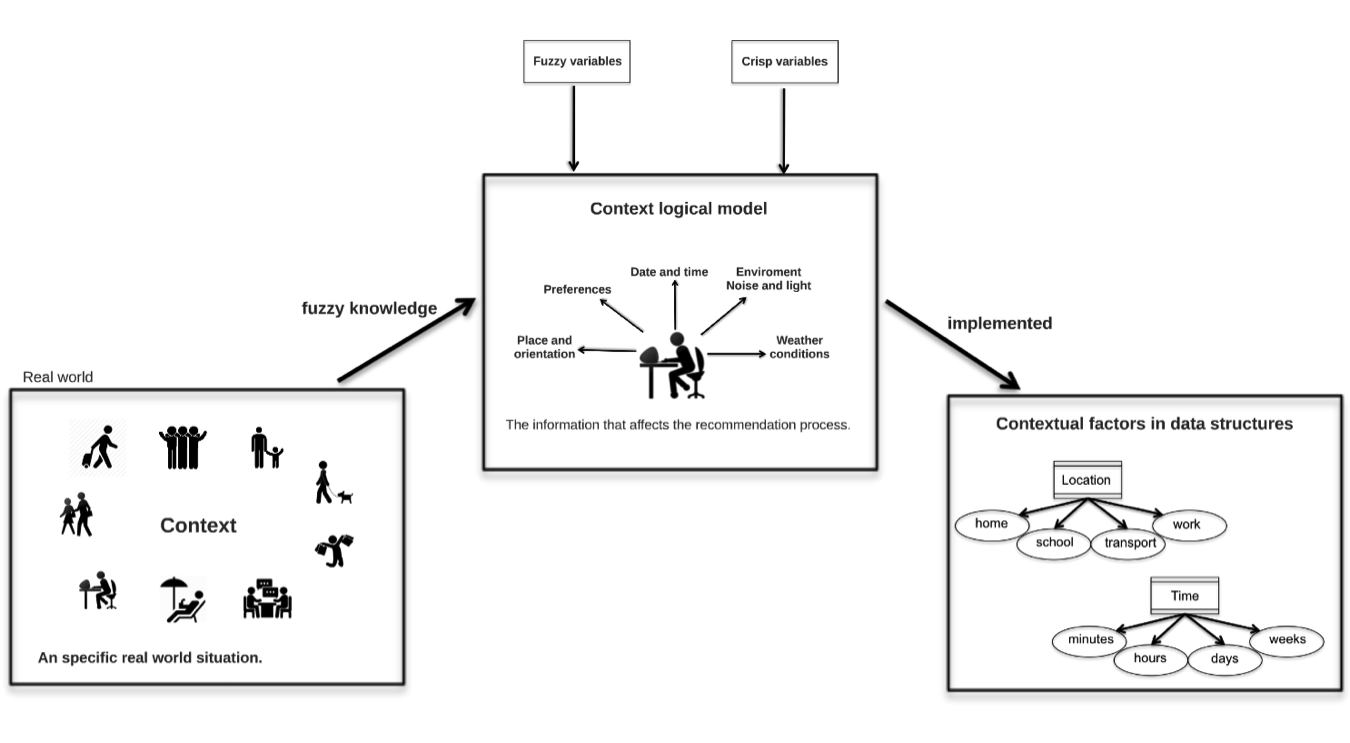
\includegraphics[width=1.0\textwidth]{img/context-scheme.png}  
\small
\caption{Logical data model of context for an application.}
\label{fig:logicalmodel}    
\end{figure*} %\end{landscape}

\section{Context-awareness} \label{context-awareness}

Traditional recommender systems provides suggestions of useful items
for a certain user. The suggestion relates to various decision-making
processes, for instance, what items to buy, what music to listen to or
what on-line news to read. \textit{Item} is the general term to denote
what product or service the system recommends for each user. A
recommender system normally focuses only in a type of item
\cite{resnick1997recommender}.
The improvements of previous recommender systems are focused in the
\textit{integration of context} in its recommendation process. 
The idea of \textit{context-aware computing} is to provide
information or services for the user based in the user's situation
\cite{dey2001understanding}. In order to do that, the application 
needs to obtain situational data, process it and make use of it 
in a manner that benefits the user. \\ 
\textit{Context} is a concept not easy to define, it is related with
several disciplines that propose different definitions. For example,
the authors Bazire et.al.\cite{bazire2005understanding} compare the
context in different fields and conclude that is complicated makes a
unifying definition of context because of the nature of the concept in
the disciplines. In computer sciences Fischer\cite{fischer2012context}
defines context as \textit{``the interaction between humans and
computers in socio-technical systems that takes place in a certain
context referring to the physical and social situation in which
computational devices and environments are embedded"}. Also identifies
the important aspects to consider when the context is used: how it is
the contextual data obtained, how the context is represented and what
goals and purposes the context has when is used in a particular
application. \\
Probably the definition most used in the field of recommender systems to 
define \textit{context} is proposed by Dey\cite{dey2001understanding}:
\textit{``Context is any information that can be used to characterize
the situation of an entity. An entity is a person, place or object
that is considered relevant to the interaction between a user and  an
application, including the user and applications themselves.''}  This
definition makes it easier to define the contextual factors in a
specific application. For instance, in a tourist guide application the
entities can be companion(friends, family, couple), place of interest,
season and weather, these could be considered as relevant contextual
factors that help the recommender system to provide items adjusted the
situational data of the user.\\
\textit{Context-aware recommender systems} are gaining even more
attention because of their performance and implementation for
different domains, the  way to improve personalized recommendations
based in contextual factors is an important technique to increase the
benefits in  many domains. For instance, taking in account the
\textit{hour of the day},  or the \textit{day of the week} when
recommending restaurants could  filter out restaurants that are
currently closed or near closing time, when the user receives this
information in real time, the user has the  way for taking
alternatives of restaurants that provide services. Nowadays, many
companies are incorporating some type of context (as time, location or
companion) in their recommendation engines, the application can be
found in fields such as e-commerce\cite{schafer1999recommender}
\cite{bulander2005enabling}, music\cite{ricci2012context}
\cite{baltrunas2011incarmusic} \cite{huq2010automated}, places of
interest\cite{baltrunas2012context},
movies\cite{eyjolfsdottir2010moviegen}, vacation
packages\cite{liu2011personalized} \cite{liu2014cocktail},  travel
guides\cite{savage2012m}, e-learning\cite{ortigosa2010entornos}  and
restaurants\cite{chu2013chinese}.\\
Plus, context can be used to improve the user satisfaction  in
recommender systems, thus the quality and accuracy of predictions  
is improved too. \\
The proposed method uses three recommendations techniques:
\begin{enumerate} 
\item \textit{Fuzzy Inference System}, this a rule based recommender
defined by an expert in the domain, it considers the following
variables: \textit{ratings average: low,medium and high},
\textit{price of restaurant: cheap, average and expensive}, and
\textit{number of ratings of item: few, several and many}, these
variables are used to infer how relevant a restaurant is for the user.
This recommendation is based on the popularity of each item in the
user community.
\item \textit{Content-based technique} utilizes the item profiles 
to compare how \textit{similar} is an item with respect to 
another, i.e. restaurants that are \textit{similar} (same cuisine, 
ambient, price range) to others that the user has rated high. 
The idea is to find items with similar features. 
\item \textit{Collaborative filtering technique} is based on the user
profile to identify user's preferences and to find neighbors that
have the same tastes. The recommendation consist in the suggestions of
other users with similar tastes that rated restaurants again in a
similar way but where have not been rated by the current user. A Top-N
list of restaurants is obtained to recommend for the user.
\end{enumerate} 
The results of the three techniques are a list of recommendations for
the user, later, these recommendations are adjusted in context. This
is the last step and is represented as \textit{context filter} in the
method, then the recommender system obtains a list of contextualized
recommendations. \\
In the method, each technique works simultaneously to obtain
recommendations, the hybrid method allows to generate suggestions even
without user information, i.e., using content-based technique or the
fuzzy inference system, so the system faces the cold-start or the
overspecialization problem using these thechniques, these problems are
described in section \ref{coldstart} and 
\ref{overspecialization}, respectively.\\
To test the performance were made several experiments that validate
the method, the algorithms were tested using contextual datasets and
the number of contextual factors used varies according the information
provided in the dataset. The goals of the experiments were to observe
the context role in the performance of the algorithms, what contextual
factors matter for users in a specific situation, how recommendations
are improved using context and, the accuracy in recommendations.
Chapter \ref{results} shows the results, discussion about results is
explained in each section.\\
Another important metric is the \textit{user satisfaction}, two
metrics were used to measure it: \textit{task-success} and \textit
{time-on-task}. These metrics allow to measure the user experience,
this offers so much more than just simple observation.\\ Usability
metrics can help reveal patterns that are hard or even impossible to
see. Evaluating software with a small sample size usually reveals the
most obvious usability problems\cite{albert2013measuring}.\\ Then, as
a general rule of thumb, during the early stages of design, it needs
fewer participants to identify the major usability issues. As the
design gets closer to completion, the tests should include more
participants to identify the remaining
issues\cite{albert2013measuring}.\\ 
Following this precept, ten representative users were selected to test
the system, subsequently, it was realized an analysis about the system
performance and issues presented in the user interaction. The chapter
\ref{evaluation} explains the process to evaluate the system and the
results obtained.
%%HECHO.

\section{Aims}

The contribution is to propose a method for context-aware recommender
systems using different techniques of recommendation, another aim is
to provide a \textit{useful knowledge} to utilize a hybrid method that
is easily implemented in different domains such as e-learning, movies,
music, tourism, etc. In this particular case, the restaurants domain
is used as a case of study to test the method.\\
Another important contribution is the use of fuzzy rules in the
proposed method, this allows the use of linguistic information closer
to the real context of the people, i.e., the method uses this
technique to analyze the user preferences and get recommendations
based in that information. For instance, the system provides a list of
range of prices, this allows the user to select a specific range of
price to get recommendations adjusted for the tag selected.\\ In order
to support the achievement of contributions, the particular aims of
this thesis are following:
\begin{itemize}  
\item Elaborate an analysis about state of the art in the field
of context-aware recommender systems through  the revision of
literature. 
\item Select the algorithms that represent alternatives of
solution for the problem in order to test their perfomance in different
domains.
\item Realize experiments with the proposed algorithms.
\item Based in previous experiments and results, to propose a hybrid
method and apply it in a case of study.
\item Define the fuzzy inference system that serves as recommender
technique in the proposed method, as well as the variables and fuzzy
rules involved.
\item Develop a prototype of context-aware recommender system 
using the proposed method.
\item To select the algorithms that represent alternatives of
solution for the problem to evaluate their perfomance in different
domains.
\item Evaluate the performance of the algorithms using 
different datasets in order to observe the system behaviour 
for each particular case.
\item Propose a hybrid method for context applied in a case of
study.
\item Develop a prototype of context-aware recommender system 
using the method in a specific domain.
\item Evaluate the proposed method using usability metrics.
\end{itemize} 

\section{Outline}

The rest of this thesis is organized as follows: 
\begin{itemize}  
\item \textbf{Chapter \ref{stateoftheart}} describes an in-depth study
of current background and related work is presented to give a general
overview of recommender systems and their evolution in recent years.
This study includes the traditional recommender systems, their methods
and techniques to improve recommendations, as so the problems to face
up this systems. Subsequently, the hybrid methods used in different
applications, their strenghts and weaknesses for each hibridation and
the domains of application. Finally, context-aware recommender systems
are mentioned, in the same way, we speak about the advantages and
disadvantages of the use of context in recommender systems.
\item \textbf{Chapter \ref{background}} describes the fundamental
concepts required to understand the proposed method.
\item \textbf{Chapter \ref{method}} presents a model of context-aware
recommender system, the proposed method  involves the paradigm of
post-filtering in a restaurants domain. This chapter include the
overall explanation of data models and  the method functionality, as
well as its components for this case of study.
\item \textbf{Chapter \ref{results}}, the general results of different
projects involved are presented along with the validation of every
experimentation. The experiments were realized using different
datasets and different algorithms in order to find an optimal manner
to reduce the error level. This chapter also details the results for
each experiment from a point of view of scientific results.
\item \textbf{Chapter \ref{evaluation}}, after the development of
context-aware recommender system, it was evaluated the impact of
context in recommendation process. This chapter describes the
usability tests that were applied on-line in order to evaluate the
satisfaction of users. Details of the environment and the
characteristics of the tests are described, as well as the results of
each one.
\item \textbf{Chapter \ref{conclusions}}, this chapter concludes with a
summary of its contributions and  its limitations. It discuss final
conclusions and the proposals for the future work.
\end{itemize}  

At the end, this thesis includes several appendices describing
detailed technical aspects of the context-aware recommender system
\textit{(appendix \ref{appendixc})}, the pseudocode of algorithms
\textit{(appendix \ref{appendixa})}, interfaces of the prototype of
context-aware recommender system \textit{(appendix \ref{appendixd})}
and experiment study materials \textit{(appendix \ref{appendixb})}.

\chapter{State of the art} \label{stateoftheart}

%Propongo una Sección de RS tradicionales y
%otra de Context Aware


In this section the state of the art in conventional and
context aware recommender systems is presented. 

As a technology recommender systems have beem applied 
in many domains, and sometimes they represent the  key
technology for the success of web and mobile applications.

%Debemos presentar el SoA con cierto orden, ya sea como una linea
%del tiempo, empezando de los primeros trabajos a los más recientes
%o organizarlo por dominios, tecnologías etc. Voy a 
%clasificar los diferentes trabajos y después los organizamos
% 


%Tipo de información: Social, Aplicación Social 
%Tags
Some works utilize social information to recommend such
as Manca et.al.\cite{manca2014mining} where the friend recommender
system is applied in the social bookmarking domain, its goal was to
infer the interest of users from content selecting the available
information of the user behavior and analyzing the resources and the
tags bookmarked for each user, therefore the recommendations are
through mining user behavior in a tagging system, analyzing the
bookmarks tagged of the user and the frecuency for each used tag. 
%Keywords
J.Yao et.al.\cite{yao2012product} proposes a new product recommendation
approach for new users based on the implicit relationships between
search keywords and products. The relationships between keywords and
products are represented in a graph and relevance of keywords to
products is derived from attributes of the graph.
%Semantic
The relevance
information is utilized to predict preferences of new users. J.
Golbeck et.al.\cite{golbeck2006filmtrust} presents FilmTrust, a
website that integrates Semantic Web-based social networks, augmented
with trust, to create prediction movie recommendations. Trust takes on
the role of a recommender system forming the core of an algorithm to
predict a rating for recommendations of movies. This is an example of
how the Semantic Web, and Semantic trust networks in particular, can
be exploited to refine the user experience. \\  
%Eso de pros y cons me lo han criticado, me pedían algo más específico
%Este párrafo está bien por que se organiza por problema que atacan las
%propuestas
Traditional recommender techniques has its pros and cons, for
instance, the ability to handle data sparsity and cold-start problems
or considerable ramp-up efforts for knowledge acquisition and
engineering. Establish hybrid systems that combine the strengths of
algorithms and models to overcome some of the shortcomings and
problems has become the properly manner to improve the difficults for
each algorithm.
%Turistas
An example is presented by L.Castro et.al.\cite{castro2012prototype} 
a hybrid recommender system for the province of San Juan, Argentina, 
to recommend tourist packages  based on preferences and interest 
of each user, artificial intelligence
techniques are used to filter and customize the information. The
prototype of recommender system utilizes three techniques to
recommend: demographic, collaborative and content-based. The goal is
to recommend tourist packages that matches with the user profile.
%Restaurantes
L. Martinez et al.\cite{martinez2009reja} presents REJA, a hybrid
recommender system that involves collaborative filtering and
knowledge-based model, that is able to provide recommendations in some
situation for user; besides it provides georeferenced information
about the recommended restaurants.
%De los primeros
Balabanovic et.al.\cite{balabanovic1997fab} presents
Fab, a hybrid recommender system for automatic recognition of
emergent issues relevant to various groups of users. It also enables
two scaling problems, pertaining to the rising number of users and
documents, to be addressed. Claypool et.al.\cite{claypool1999combining} 
presents P-Tango system that utilizes content-based and collaborative
filtering techniques, it makes a prediction through the weighted
average that includes content-based prediction and collaborative
filtering prediction. The weights of predictions are determined on a
per-user basis, allowing the system to determine the optimum mixture
of content-based and collaborative recommendation for each user.
Pazzani M.\cite{pazzani1999framework} presents Entree as a hybrid
recommender system that it does not use numeric scores, but rather
treats the output of each recommender (collaborative, content-based
and demographic) as a set of votes, which are then combined in a
consensus scheme. The recommender system includes information such as
the content of the page, ratings of users and demographic data about
users. 
%Hibridos
Others works with hybrid recommender systems are ProfBuilder
\cite{al1999semantic}, PickAFlick\cite{burke1999integrating}  and
\cite{tran2000hybrid}, where are presented multiple recommendation
techniques. Usually, recommendation requires ranking of
items or selection of a single best recommendation, at this point some
technique must be employed to recommend. \\ 
Traditional recommender systems such as above mentioned, tend to use
simple user models. For example, user-based collaborative filtering
generally models the user as a vector of item ratings. As additional
observations are made about users’ preferences, the user models are
extended, and the user preferences is used to generate
recommendations. This approach, therefore, ignores the notion of any
specific situation, the fact that users interact with the system
within a particular context and  that preferences of items might 
change in another context. 
%Contextuales 
Overall, the context is able to make the recommender system be 
powerful that is adaptable to the changing user's situation.\\
The context is defined in the domain of the application and the system
has a context model that provides the information for the recommender
system. For instance Ricci et.al. \cite{baltrunas2011incarmusic} uses
the context in music domain using a model-based paradigm, in this
context-aware recommender system the context was defined as a set of
independent contextual factors(independent in order to get a
mathematical model) such as \textit{driving style, road type,
landscape, sleepiness, traffic conditions, mood weather and natural
phenomena} to specifies the relevant context for the music
recommendation. In order to estimate the relevance of selected
contextual factor, the users were requested to evaluate music tracks
in different contextual situations for each genre. The prediction
takes in account this relevance to recommend music tracks prefered by
the user according the genre and the contexts mentioned.In
restaurant domain Chung-Hua et al.\cite{chu2013chinese} presents a
context-aware recommender system for mobiles using a post-filtering
paradigm, the architecture involves a model client-server that works
with a request of data in the client side for the server side.
Subsequently, taking in account the contextual factors to filter the
properly restaurants to recommend. The context-aware recommender
system uses such as contextual factors \textit{location and season}, 
also utilize the user preferences to personalize the recommendations
in the user context.
Baltrunas et.al.\cite{baltrunas2011context} presents ReRex for tourism, 
a context-aware recommender system based in a model-based paradigm, the system
recommends and provides explanations about the why the places of
interest(PoI) are recommended. The proposed model computes a
personalized context dependent rating estimation. Subsequently, in
order to generates the explanation of recommendation the system uses
the factor that in the predictive model has the lasgest positive
effect on the rating prediction for the point of interest. The set of
contextual factors considered in ReRex are \textit{distance},
temperature, weather, season, companion, time day, weekday,
crowdedness, familiarity, mood, budget, travel length, transport and
travel goal. The main issue in ReRex system is the low user
satisfaction because of the explanations not able to be understood,
however the users recognize that the explanation is a very important
component that it influence the system acceptance. Noguera et. al.
\cite{noguera2012mobile} presents a context-aware recommender system
for tourism based in REJA that utilizes the location through a 3D-GIS
system, the application uses progressive downloading and rendering of
3D maps over mobiles networks. It is also in charge of tracking the
user’s location and speed based on GPS and the requesting. The system
utilizes pre-filtering and post-filtering paradigm. Pre-filtering is
used to reduce the number of items considered for the recommendation
according to the user’s location, and  post-filtering is applied to
re-rank the previous top-N list according to the physical distance
from the user for each recommended restaurant. The disadvantage in this
system is the lack of user reviews, because the recommendations are
based only in the location point without consider the experience of
other diners concerning the recommended restaurant. 
Cena et al.\cite{cena2006integrating} presents a tourist guide for
context in intelligent content adaptation. UbiquiTO system is a
tourist guide that integrates different forms of context-related
adaptation: for media device type, for user characteristics and
preferences, for the physical context of the interaction. UbiquiTO uses
a rule-based modeling approach to adapt the content of the provided
recommendation, such as the amount, type of information and features
associated with each recommendation. 
Bulander et.al\cite{bulander2005comparison} presents the MoMa-system that
offers proactive recommendations using a post-filtering approach for
matching order specifications with offers. When creating an order, the
client application will automatically fill in the appropriate physical
context and profile parameters, for example, \textit{location} and \textit{weather},
then, for example, the facility should not be too far away from the
current location of the user and beer should not be
recommended if it is raining. On the other side, advertisers’
suppliers put offers into the MoMa-system. These offers are also
formulated according to the catalogue. When the system detects a pair
of context matching order and offer, the end user is notified, in the
preferred manner (for example, SMS, email). At this point, the user
must decide whether to contact the advertiser to accept the offer.
Finally, Schifanella et al.\cite{schifanella2008mobhinter} develops
Mob-Hinter, a \textit{context-dependent} distributed model,where a user device
can directly connect to other mobile devices that are in \textit{physical
proximity} through ad-hoc connections, hence relying on a very limited
portion of the users’ community and just on a subset of all available
data (pre-filtering). The relationships between users are modeled with
a similarity graph. MobHinter allows a mobile device to identify the
affinity network neighbors from random ad-hoc communications. The
collected information is then used to incrementally refine locally
calculated predictions, with no need of interacting with a remote
server or accessing the Internet. The Recommendations are computed
using the availables rating of the user neighbors.
Abowd et. al. presents Cyberguide project \cite{abowd1997cyberguide},
which encompassed several tour guide prototypes for different handheld
platforms. Cyberguide provided tour guide services to mobile users,
exploiting the contextual knowledge of the user’s current and past
locations in the recommendation process. The PECITAS system
\cite{tumas2009personalized} presented by Thumas offers location-aware
recommendations for personalized point-to-point paths. The paths are
illustrated by listing the various connections that the user must take
to reach the destination using public transportation and walking. An
interesting aspect of PECITAS is that, although an optimal shortest 
path facility is incorporated, users may be recommended alternative 
routes that pass through several attractions, given that
their specified constraints (e.g. latest arrival time) and travel-related 
preferences (maximum walking time, maximal number of transport
transfers, sightseeing preferences, etc) are satisfied. Yu and Chang
presents LARS \cite{yu2009personalized} which supports personalized
tour planning using a rule-based recommendation process. This system
packages ‘where to stay’ and ‘where to eat’ features together with
‘typical’ tourist recommendations for sightseeing and activities. For
instance, recommended restaurants (selected based on their location,
menu, prices, customer rating score, etc) are integral part of the
tour and the time spent for lunch/dinner is taken into account to
schedule visits to attractions or to plan other activities.
Savage et. al. presents  "I'm feeling LoCo" system \cite{savage2012m}
that proposes a ubiquitous location­ based recommendation algorithm
that focuses on user experience by considering user preferences, time,
location and similarity measures automatically, having Foursquare as a
dataset. We also focus on user experience and aim that user input is
minimal. The information  om the user's social network, form of
transportation and phone's sensors is inferred to provide
recommendation of places  om the dataset.
Reddy et.al\cite{reddy2006lifetrak} presents LifeTrack system that
incorporates sensor information into song selection. The songs are
represented in terms of tags that the user assigns in order to link
the songs to the appropriate contexts in which they should be played.
User feedback is incorporated to make a song more or less likely to
play in a given context. Context considered relevant to song selection
includes location, time of operation, velocity of the user, weather,
traffic and sound. User locations and velocity are determined by GPS.
Location information includes tags based on zip code and whether the
user is inside or outside (inferred by the presence or absence of a
GPS signal). The times of the day are divided out into configurable
parts of the day (morning, evening, etc). The velocity is abstracted
into one of four states: static, walking, running and driving. Use of
accelerometers are planned to enable indoor velocity information. If
the user is driving, an RSS feed on traffic information is used to
typify the state as calm, moderate or chaotic. If the user is not
driving, a microphone reading is used for the same purpose.
Additionally, an RSS feed provides a meteorological condition (frigid,
cold, temperate, warm or hot).\\ The table \ref{tab:stateoftheart}  
describes examples of contextual factors in different domains 
of application, specifies the contextual factors considered 
such as  part of the context, the methodology for each 
application and  kind of devices.

\begin{sidewaystable}[]
  \caption{Comparison of context-aware recommender systems.}
    \label{tab:stateoftheart}
  \bigskip
    \centering\small\setlength\tabcolsep{2pt}
        \hspace*{-1cm}\begin{tabular}{p{3.5cm} p{6cm} p{4cm} p{3cm} p{3cm} }%{l l l l l}
           \toprule
             \textbf{Application} &\textbf{Contextual Factor} &\textbf{Domain} &\textbf{Paradigm} &\textbf{Device}  \\ \hline

           \midrule
             \textbf{CoMoLE} & \textbf{Time, available time, place, device, level of knowledge, learning style.} & \textbf{E-learning} & \textbf{Pre-filtering} & \textbf{Mobiles, PC, laptop.}   \\ \hline 

             \textbf{Moma-System} & \textbf{Location, time.} & \textbf{E-commerce} & \textbf{Post-filtering} & \textbf{PC, laptop.}  \\ \hline

             \textbf{UbiquITO} & \textbf{Season, time, temperature.} & \textbf{Tourism} & \textbf{Post-filtering} & \textbf{Mobiles} \\ \hline

             \textbf{ReRex} & \textbf{Distance of the point of interest,  temperature, weather, season, weekend, companion, travel goal, transport.} & \textbf{Tourism} & \textbf{Model-based} & \textbf{Mobiles} \\ \hline

             \textbf{LifeTrack} & \textbf{Location, time, day of the week, traifc noise(level), temperature, weather.} & \textbf{Music} & \textbf{ Post-filtering} & \textbf{PC, Mobiles.} \\ \hline

             \textbf{CARS} & \textbf{Location and season.} & \textbf{Restaurants} & \textbf{Post-filtering} & \textbf{PC, laptop.} \\ \hline

             \textbf{InCarMusic} & \textbf{Driving style, road type, landscape, sleepiness, traffic conditions, mood weather and natural phenomena.} & \textbf{Music} & \textbf{Model-based} & \textbf{Mobiles} \\ \hline

            \textbf{REJA} & \textbf{Location.} & \textbf{Restaurants} & \textbf{Pre-filtering and Post-filtering} & \textbf{PC, laptop, mobiles.} \\ \hline

            \textbf{CiberGuide} & \textbf{Location, time, weather.} & \textbf{Tourism} & \textbf{Post-filtering} & \textbf{Mobiles} \\ \hline

            \textbf{PECITAS} & \textbf{Location, routes.} & \textbf{Transport} & \textbf{Post-filtering} & \textbf{Mobiles} \\ \hline

            \textbf{LARS} & \textbf{Tourists’ location and time.} & \textbf{Tourist packages} & \textbf{Post-filtering} & \textbf{Mobiles} \\ \hline

            \textbf{I'm feeling LoCo} & \textbf{Location, transportation.} & \textbf{Tourism} & \textbf{Model-based} & \textbf{Mobiles} \\ \hline

            \textbf{MOPSI} & \textbf{Location} & \textbf{Tourism and transport} & \textbf{Post-filtering} & \textbf{Mobiles} \\ \hline

           \bottomrule
        \end{tabular}\hspace*{-1cm}
\end{sidewaystable}









%% La letra n con tilde es: 'n.
\chapter{Background}\label{background}

In this chapter the fundamental concepts related this work are presented:
Formal definitions referring to fuzzy systems, contextual factors and
recommender system techniques used by the proposed method.
%--------------------------------------------------------------
%Agregue la seccion de logica difusa del articulo que me mando.

\section{Production systems and fuzzy models}

A central aspect of the proposed method is the use of both fuzzy logic and
fuzzy inference systems, in this section formal definitions of
these models of knowledge representation are presented.  

\subsection{Traditional Production Systems}
Production Systems represent knowledge in form of rules, which specify
actions that will be executed when certain conditions are met. In these 
systems Experts in a certain domain identify a set of rules based 
on their experience to
resolve different kinds of problems. Also known as rule based systems,
many implementations consist of mainly these three
components \cite{brachman1992knowledge} \cite{konar2006computational}:
\begin{enumerate}   
\item \textbf{Production Rules (PR)}. A set of
production rules (also known as \textit{IF-THEN} rules) having a two part
structure; the antecedent, conformed by a set of conditions and a
consequent set of actions. 
\item \textbf{Working Memory (WM)}.
Represents the current knowledge or facts that are known to be true so
far. These facts are tested by the antecedent conditions of the rules
and the consequent part can change them. 
\item \textbf{Inference Engine (IE)}. 
This interpreter matches the conditions in the
production rules with the data/instantiations found in the WM,
deriving new consequences.
\end{enumerate}
The basic operation of these systems is described as a cycle of 
three steps \cite{brachman1992knowledge}:
\begin{enumerate}
\item \textbf{Recognize}: Find which rules are satisfied by 
the current WM. The antecedent part of the productions consists 
of a set of clauses connected by AND operators, when all these 
clauses have matching data on the WM the production has a chance 
of firing.
\item \textbf{Conflict Resolution}: Only one production can be 
fired at a time, so when two or more rules can be fired concurrently 
a conflict occurs. Among the production rules found in the first 
step, choose which rules should fire.
\item \textbf{Actions}: Change the working memory by performing 
the actions specified in the consequent part of all the rules 
selected in the second step. Changes occur by adding or 
deleting elements of the WM.
\end{enumerate}
This cycle continues until no further production rules can be fired.
This control strategy is data driven because whenever the antecedent
part is satisfied the rule is recognized, this strategy is also named
chain-forward. Other strategy is chain-backward in which case the work
is done from the conclusion to the facts, to chain-backward, goals in
the WM are matched against consequents of the production
rules.\\A drawback that has been recognized in these traditional
productions systems, is that some times rules are not fired in the
Recognize step because no appropriate match exists in the WM. Partial
matching of rules is not possible and this can be a limitation in some
systems because premature termination of the cycle is not desired. An
approach to handle partial matching is using fuzzy logic
\cite{konar2006computational}. In the next section a review of the
extension of production systems with fuzzy logic is presented.\\

\subsection{Fuzzy Production Rules}

Fuzzy production rules use fuzzy logic sets to characterize the
variables and terms used in the propositions of the rules. Fuzzy
production rules or fuzzy \textit{IF-THEN} rules are expressions of
the form \textit{IF} antecedent \textit{THEN} consequent, where the
antecedent is a proposition of the form \textit{"x is A"} where
\textit{x} is a linguistic variable and \textit{A} is a linguistic
term. The truth value of this proposition is based on the matching
degree between \textit{x} and \textit{A}. Propositions are connected
by \textit{AND}, \textit{OR} and \textit{NOT} operators. Some
implementations of fuzzy rule-based systems also include other kinds
of data types in their propositions, for example the FLOPS system
includes fuzzy numbers, hedges, and non fuzzy data types (integers,
strings and float) \cite{siler2005fuzzy}. Depending on the form of the
consequent, two main types of fuzzy production systems are
distinguished \cite{babuvska1996fuzzy}:
\begin{itemize}  
\item \textbf{Linguistic fuzzy model}: where both the antecedent 
and consequent are fuzzy propositions.
\item \textbf{Takagi-Sugeno fuzzy model}: the antecedent is a fuzzy 
proposition; the consequent is a crisp function.
\end{itemize}  
As before, other non-fuzzy consequents can also be implemented, like
the execution of commands or the addition of new data.\\
\textbf{Linguistic Variables (LV)} are variables that can be assigned
linguistic terms as values, i.e. if we define a linguistic variable
\textit{SPEED} we can assign it the linguistic terms \textit{SLOW},
\textit{MEDIUM} or \textit{FAST}. The meaning of these linguistic
terms is defined by their membership functions (MF). \textit{LV} can
be defined as a \textit{5-tuple} \textit{LV=}$<v,T,X,g,m>$ where
\textit{v} is the name of the variable, \textit{T} is the set of
linguistic terms of \textit{v}, \textit{X} is the domain (universe) of
\textit{v},\textit{g} is a syntactic rule to generate linguistic terms,
\textit{m} is a semantic rule that assigns to each term \textit{t} its
meaning \textit{m(t)}, which is a fuzzy set defined in \textit{X}.

\subsection{Fuzzy Inference Systems}

\textit{Fuzzy Inference Systems} (FISs) also called \textit{Fuzzy
Models} are fuzzy production systems used for modeling input-output
relationships. From this input-output view, Babuŝka
\cite{babuvska1996fuzzy} describes these systems as \textit{``flexible
mathematical functions which can approximate other functions or just
data (measurements) with a desired accuracy"}. Fuzzy Productions Rules
define the relationship between input and output variables. Input
variables are defined in the antecedent part of the rule and the
consequent part defines the output variables. These FISs are used
mainly in control systems, and are basically composed of five
modules\cite{babuvska1996fuzzy}:
\begin{enumerate}  
\item \textbf{Rule Base.} The set of fuzzy production rules.
\item \textbf{Database.} Where the membership functions are defined.
\item \textbf{Fuzzy Inference Engine.} This module executes the 
fuzzy inference operations.
\item \textbf{Fuzzifier.} This interface transforms the inputs 
of the systems (numerical data) into linguistic values.
\item \textbf{Defuzzifier.} This interface transforms the fuzzy 
results into numerical data.
\end{enumerate}
Usually the Rule Base and Data Base modules are collectively 
called the Knowledge Base module. The steps involved in fuzzy 
inference in a FIS are \cite{dubois1980fuzzy}:
\begin{enumerate} 
\item Compare the input variables with the membership functions 
in the antecedent, to obtain the membership values of each 
linguistic term. This step is frequently called fuzzification.
\item Compose through a specific T-Norm operator (mainly max-min 
or max-product) the membership values to obtain the degree of 
support of each rule.
\item Generate the qualified consequence (fuzzy or numeric) of 
each rule depending on the degrees of support. These outputs 
are then aggregated to form a unified output.
\item Then the output fuzzy set is resolved or defuzzified 
to a single numeric value.
\end{enumerate} 
Three main inference systems can be described:
\begin{itemize} 
\item \textbf{Tsakumoto}: The output is the average of the 
weights of each rule numeric output, induced by the degree of 
support of each rule, the min-max or min-product with the 
antecedent and the membership functions of the output. The 
membership functions used in this method must be 
non-decrease monotonic. 
\item \textbf{Mamdani}: The output is calculated by applying 
the min-max operator to the fuzzy output (each equal to the 
minimum support degree and the membership function of the rule). 
Several schemes have been proposed to choose the numeric output 
based on the fuzzy output; these include the centroid area, 
area bisection, maximum mean, maximum criteria.
\item \textbf{Sugeno}: The fuzzy production rules are used. The 
output of each rule is a linear combination of the input 
variables plus a constant term, and the output is the average 
of the support degree of each rule.
\end{itemize} 
%%-----------------------------------------------------------


\section{Context}
People transmit ideas to each in a complex way. This
is due to many factors such as: the richness of the language shared, the common
understanding of how the world works, and an implicit understanding of
situations in daily life. When people talk, they are able to use implicit
situational information (contextual information), to increase the
conversational bandwidth. \\Unfortunately, this ability to transmit
ideas does not transfer well to persons interacting with computers. In
traditional interactive computing, users have poor mechanisms for
providing input to computers. Consequently, computers are not
currently enabled to take full advantage of the context of the 
human-computer dialogue. By improving the computer's access to context, 
we increase the richness of communication in a human-computer interaction
enabling the development of more useful computational 
services.\\
In order to use context effectively, we must define what context
is and how it can be used. An understanding of \textit{how context can
be used} will help application designers to determine what 
context-aware behaviours to use in applications\cite{dey2001understanding}.\\
To stablish a specific definition of \textit{context} that can be used
in the \textit{context-aware} computing field, is necessary to review
how researchers define the context in their own work. Schilit and
Theimer\cite{abowd1999towards} refer to context as \textit{location},
\textit{identities of nearby people and objects}, and \textit{changes
to those objects}.\\
This type of definitions that define context by example
are difficult to apply when developers try to determine whether a type of
information not listed in the definition is part of the context or not, 
as it is not clear how it can be used by the definition.\\ 
Schilit et al.\cite{schilit1994context} affirms that the most important
aspects of context are: \textit{where you are}, \textit{who you are
with}, and \textit{what resources are nearby}.
Pascoe\cite{pascoe1998adding} defines context to be the
\textit{``subset of physical and  conceptual states of interest to a
particular entity"}.\\
These definitions are too general, context is all about the
whole situation relevant to an application and its set of users. It is
complicated enumerate which aspects of all situations are important,
as this will change from situation to situation. For this reason and
for the purpose of this thesis, the definition of context
proposed by Dey\cite{dey2001understanding} has been adopted (see section 
\ref{context-awareness}). \\However, another important aspect 
is to stablish a meaningful classification that covers the 
characteristics that describe the contextual factor.\\
Dourish\cite{dourish2004we} has distinguished between two different
views of context: the \textit{representational view} and the
\textit{interactional view}. The \textit{representational view} makes
four key assumptions: context is a \textit{form of information}, it is
\textit{delineable}, it is \textit{stable}, and it is
\textit{independent} from the underlying activity. In this view,
context can be described using a set of observable attributes that are
known a priori. Furthermore, the structure of these contextual
attributes does not change over time. The \textit{interactional view},
takes a different stance on the key assumptions made by the
representational view. In the interactional view, the scope of
contextual features is defined dynamically, and it is occasioned
rather than static. Rather than assuming that context acts as a set of
conditions under which an activity occurs, this view assumes a
cyclical relationship between context and activity, where the activity
gives rise to context and the context influences activities.\\
Context should include information to allow systems to use contextual
information about users and their situation, enabling the system 
to provide users personalised and contextual services. The importance of
context lies in the  assumption of the influence of \textit{contextual
factors} that matter for users when they decide, choose or discard an
item.\\
In the real world, the context in a situation is involved in the
\textit{environment} of the people, the \textit{entities} belong at
the \textit{situational information}, but an entity  becomes in a
\textit{contextual factor} when its information \textit{affects} the
recommendation process, therefore, the entity and its values of 
domain will be involved in the process such as a contextual factor.\\
The domain values of a contextual factor change over time, in
real life the situation occurs when we decide that, for instance,
we like a kind of clothes and the next day, for a any reason we don't
like it anymore. As for the representation of the \textit{"change of time"} , a data 
model of \textit{time} should be specified in a way that the system
\textit{interprets} time as a data structure (for instance weeks, 
days, hours, minutes, seconds, etc.). \\
Assuming the existence of certain contextual factors such as
\textit{time}, \textit{location} and \textit{purchasing purpose} that
are identified in the context of recommendations,
Adomavicious\cite{adomavicius2011context} proposes two important
aspects that highligh when different kinds of context are defined:
\textit{what a recommender system may know about these contextual
factors} and, \textit{how contextual factors change over time}.\\ \\

A recommender system can have different types of knowledge, which may
include  the exact list of all the relevant factors, their structure,
and their values, about the contextual factors. Depending on what
exactly the system knows (that  is, what is being observed),
Adomavicious categorizes the knowledge of a recommender system about
the context as the following:
	\begin{itemize}
	\item \textbf{Fully observable}: The contextual factors relevant to the 
	application, as well as their structure and their values at the time when 
	recommendations are made, are known explicitly. For example, when
	recommending the purchase of a certain product, like a shirt, the 
	recommender system may know that only the \textit{Time}, \textit{PurchasingPurpose}, 
	and \textit{ShoppingCompanion} factors matter in this application. Further more, 
	the recommender system may know the structure of all three contextual 
	factors, such as having categories of \textit{weekday}, \textit{weekend}, 
	and \textit{holiday} for \textit{Time}. Further, the recommender system 
	may also know the values of the contextual factors at the recommendation 
	time, for instance, \textit{when this purchase is been made}, 
	\textit{with whom}, and \textit{for whom}.
	\item \textbf{Partially observable}: Only some of the information about 
	the contextual factors described above, is explicitly known. For example, 
	the recommender system may know all the contextual factors, such as Time, 
	PurchasingPurpose, and ShoppingCompanion, but not their structure. Note that 
	there can possibly be different levels of \textit{"partial observability"}. 
	\item \textbf{Unobservable}: No information about contextual factors is 
	explicitly available to the recommender system, and it makes recommendations 
	by utilizing only the latent knowledge of context in an implicit manner. 
	For example, the recommender system may build a latent predictive model, 
	such as hierarchical linear or hidden Markov models, to estimate unknown 
	ratings, where unobservable context is modeled using latent variables.
	\end{itemize}
\textbf{How contextual factors change over time.} Depending on whether 
contextual factors change over time or not, two categories are proposed: 
	\begin{itemize}
	\item \textbf{Static}: The relevant contextual factors and their structure
	remain the same (stable) over time. For example, when recommending the
	purchase of a certain product, such as a shirt, we can include the
	contextual factors of Time, PurchasingPurpose and ShoppingCompanion 
	without change during the entire lifespan of the purchasing recommendation
	application.
	\item \textbf {Dynamic}: This is the case when the contextual factors 
	change in some way. For example, the recommender system (or the 
	system designer) may realize over time that the \textit{ShoppingCompanion} 
	factor is no longer relevant for purchasing recommendations and may 
	decide to drop it. Furthermore, the structure of some of the contextual
	factors can change over time, for instance, new categories can be
	added to the \textit{PurchasingPurpose} contextual factor over time.
	\end{itemize}
On the other hand, Fling\cite{fling2009mobile} generalizes four types of
contexts that can be used in different applications:  
\begin{itemize}  
\item \textbf{Physical context}: representing the time, position, and
activity of the user, but also the weather, light, and temperature
when the recommendation is supposed to be used.  
\item \textbf{Social context}: representing the presence and role 
of other people (either using or not using the application) around 
the user and whether the user is alone or in a group when using 
the application. 
\item \textbf{Interaction media context}: describing the device used to
access the system (for example, a mobile phone or a kiosk) as well as
the type of media that are browsed and personalized. The latter can be
ordinary text, music, images, movies, or queries made to the
recommender system.  
\item \textbf{Modal context}: representing the current state 
of mind of the user,  the user's goals, mood, experience, 
and cognitive capabilities. 
\end{itemize} 
Subsequently the revision of the literature of context, it is important
to mention a formal definition that describes what features it has a
context-aware system, this definition is proposed by
Dey\cite{dey2001understanding}: \textit{``a system is context-aware if
it uses context to provide relevant information and/or services for
the user, where relevancy  depends on the user's task."}\\ This
definition is closer  to the reality about behaviour of \textit
{context-aware recommender system} when incorporates contextual
information.\\  
Based in this definition, Dey proposes some characteristics 
that a context-aware application should be support:
\begin{itemize}  
\item \textbf{Presentation of information} and services to a user.
\item \textbf{Automatic execution} of a service for a user.
\item \textbf{Tagging of context} to information to support later retrieval.
\end{itemize} 
An example to explain the context in a context-aware application, for
instance, it can be an indoor mobile tour guide. Here, the entities
are the user, the application and the tour sites. We will look at two
pieces of information (weather and the presence of other people) and
use the definition to determine if either one is context. The weather
does not affect the application because it is being used for indoor activities.
Therefore, it is not context. The presence of other people, however,
can be used to characterize the user’s situation. If a user is
traveling with other people, then the sites that they visit may are
the points of interest for the user. Therefore, the presence of other
people is context because it can be used to characterize the user's
situation.

\section{Recommender systems}

\subsection{Collaborative Filtering}

The idea behind collaborative recommendation approaches is to exploit
information about past behavior or opinions of an exisiting user
community for predicting which items certain user of the system will
most probably like or be interested in\cite{jannach2010recommender}. 
Recommender systems are useful in several types of  applications,
however, their biggest impact has been mainly in ecommerce web sites
in order to personalize the information for a particular user as the
system can help to promote several items of his or her interest, thus
increasing the sales of the on-line store. In traditional
implementations a collaborative filtering algorithm (CF) takes as
input a given \textit{user-item} sparse matrix of ratings to generate a
prediction for each user-item pair indicating to what degree the
current user will like or dislike an item. Subsequently with that
information a list of the top \textit{n} recommended items for the
user can be generated. The generated list contains only those items
that have not been reviewed by the user. Different approaches are
utilized for CF such as: a) User-based nearest 
neighbor recommendation, b) Item-based nearest neighbor 
recommendation and c) Model-based recommendation.\\
\textbf{a) User-based nearest neighbor} is an approach that only 
uses the rating matrix to obtain recommendations. 
The neighborhood selection consists in taking
the \textit{k} nearest (similar) neighbors into account usind the \textit{k} threshold to
define the size of the neighborhood. A small neigborhood can not
make accurate predictions, and on the other hand if the neighborhood
is too large the information about certain nighbours could not be
significant.\\ To obtain the similarity value between a user and his
neighbors, the Pearson correlation is commonly used, taking
the values from $+1$ (strong positive correlation) to $-1$ (strong
negative correlation) to define how similar a neighbor is. The
similarity $sim(a,b)$ of users $a$ and $b$, given the rating matrix
$R$ is denoted by the following equation:
\begin{equation}\label{eq:pearson1}
\displaystyle sim(a,b) = {\sum_{p \in P}(r_{a,p} - 
\bar{r_a})(r_{b,p}- \bar{r_b}) 
\over \sqrt{\sum_{p \in P}(r_{a,p} - \bar{r_a})^2} 
\sqrt{\sum_{p \in P} 
(r_{b,p}- \bar{r_b})^2}}
\end{equation}
Where the symbol $\bar{r_a}$ corresponds to the average rating of user
$a$. Subsequently, a formula to calculate the prediction of the user
$a$ for item $p$ that also factors the relative proximity of the
nearest neighbors $N$ and $a's$ average rating $\bar{r_a}$ is denoted
by the following equation:
\begin{equation}\label{eq:prediction}
\displaystyle pred(a,b) = \bar{r_a} + 
{\sum_{b \in N} sim(a,b) * (r_{b,p}- \bar{r_b}) 
\over \sum_{b \in N} sim(a,b)} 
\end{equation}
\textbf{b) Item-based nearest neighbor} is the same idea as the \textit
{User-based} recommendation, the difference is that this approach tries to find
similar items instead of similar users to make a prediction using again only the rating
matrix as input. Then, in an \textit{item-based} recommendation is to compute
predictions using the similarity between items and not the similarity
between users. To find similar items a Cosine similarity measure is often used,
this metric measures the similarity between two
\textit{n-dimensional} vectors based on the cosine of the angle between them.
Therefore, the similarity between two items \textit{a} and \textit{b}
viewed as the corresponding rating vectors $a$ and $b$, is formally
defined as follows:
\begin{equation}\label{eq:cosine}
\displaystyle sim(\overrightarrow{a},\overrightarrow{b})= 
{\overrightarrow{a}* \overrightarrow{b} \over
|\overrightarrow{a}|*|\overrightarrow{b}| }
\end{equation}
Where the * symbol is the dot product of vectors and $|a|$ is the Euclidian
length of the vector, which is defined as the square root of the dot
product of the vector with itself.\\
%% Puedes buscar en Latex el dot product para no usar asterisco

\textbf{c) Model-based approach}, in this technique the raw data is
first processed off-line, as described for \textit {item-based}
filtering or also using some dimensionality reduction technique. At run time,
only the learned model is required to make predictions. Although a
\textit{memory-based approach} is theoretically more precise because
the full data is available for generating recommendations, such systems
face problems of scalability when for instance a database of tens of millions of
users and items are used. An example of this approach is
\textit{matrix factorization} or \textit{latent factors model},
normally used to fill a rating matrix to calculate predictions taking
in account the \textit{latent factors}.

\subsubsection{Data sparsity and cold-start problem}\label{coldstart}
In real-world applications, the ratings matrix tend to be \textit{very
sparse}(sparcity problem), as customers typically provide  ratings
for (or have bought) only a small fraction of the catalog items. In
general, the challenge in that context is thus to compute good
predictions when there are relatively few ratings available. One
straightforward option for dealing with this problem is to exploit
additional information about the users, such as gender, age,
education, interests, or other information available that can help to
classify the user. The set of similar users (neighbors) is thus based
not only on the analysis of the explicit and implicit ratings, but
also on information external to the ratings matrix. These hybrid
systems \cite{pazzani2007content}, however, are no longer
\textit{“purely”} collaborative, and also bring new questions on how to acquire
the additional information and how to combine the different
classifiers. Still, to reach the critical mass of users needed
in a collaborative approach, such techniques might be helpful in the
\textit{ramp-up phase} of a newly installed recommendation service. \\
The \textit{cold-start problem} can be viewed as a special case of
sparsity \cite{huang2004applying}. The questions here are (a)\textit{how 
to make recommendations to new users that have not rated
any item yet} and (b)\textit{how to deal with items that have not
been rated or bought yet}. Both problems can be addressed with the
help of hybrid approaches \cite{adomavicius2005toward}.  To face the
\textit{new-users problem}, one option could be to ask the user for a
minimum number of ratings before the service can be used. In this
situation the system could intelligently ask for ratings for items
that, from the view point of information theory, carry the most
information\cite{rashid2002getting}. A similar strategy of asking
the user for a gauge set of ratings is used for instance in the Eigentaste
algorithm presented in \cite{goldberg2001eigentaste}.

\subsection{Content-based algorithm}

In a content-based recommendation (CB), the task consists of determining
those items that best match the active user’s preferences. Although such an
approach must rely on additional information about items and user
preferences, it does not require the existence of a large user
community or a rating history, i.e., recommendation lists can be
generated even if there is only one single user. \\In practical
settings, technical descriptions of the features and characteristics
of an item (such as the genre of a book or the list of actors in a
movie) are more often available in electronic form, as they are
partially already provided by the providers or manufacturers of the
goods. What remains challenging, however, is the acquisition of
subjective, qualitative features. \\In domains of quality and taste, for
example, the reasons that someone likes something are not always
related to certain product characteristics and may be based on a
subjective impression of the item’s exterior design 
\cite{jannach2010recommender}.    

\subsubsection{Content representation} 

The simplest way to describe catalog
items is to maintain an explicit list of features for each item (also
often called attributes, characteristics, or item profiles). For a
book recommender, one could, for instance, use the genre, the author’s
name, the publisher, or anything else that describes the item and
store his information in a relational database system. When the user’s
preferences are described in terms of his or her interests using
exactly this set of features, the recommendation task consists of
matching item characteristics and user preferences 
\cite{jannach2010recommender}.  

\subsubsection{Vector space model}  

CB systems have historically
been developed to filter and recommend text-based items such as e-mail
messages or news. The standard approach in CB recommendation is,
therefore, not to maintain a list of \textit{meta-data
features}, but to use a list of relevant keywords that appear within
the document. The main idea, of course, is that such a list can be
generated automatically from the document content itself or from a
free-text description thereof \cite{jannach2010recommender}.

\subsubsection{Overspecialization and cold-start problem}
\label{overspecialization}

Learning-based methods quickly tend to propose
more of the same, that is, such recommenders can propose only items
that are somehow similar to the ones the current user has already
(positively) rated. This can lead to the undesirable effect that
obvious recommendations are made and the system, for instance,
recommends items that are \textit{too similar to those the user already knows}.
\\A typical example is a news filtering recommender that proposes a
newspaper article that covers the same story that the user has already
seen \textit{in another context}. The system in \cite{billsus1999personal} 
defines a threshold to filter out not only items that
are \textit{too different} from the profile but also those that are \textit{too
similar}. A general goal is to avoid the \textit{overspecialization},
therefore increasing the serendipity of the recommendation lists
that now includes “unexpected” items in which the user might be
interested, because sometimes expected items are of little value for the user.\\
The \textit{cold-start problem}, which we discussed for collaborative
systems, also exists in a slightly different form for content-based
recommendation methods. Although CB techniques do not
require a large user community, they require at least an initial set
of ratings from the user. \\In all described filtering techniques,
recommendation accuracy improves along with the number of ratings;
significant performance increases for the learning algorithms were
reported in \cite{pazzani1997learning}  when the number of ratings was
between twenty and fifty. \\However, in many domains, users might not be
willing (or is not feasible) to rate that many items before the recommender service can be
used. In the initial phase, it could be an option to ask the user to
provide a list of keywords, either by selecting from a list of topics
or by entering a free-text input.

\subsection{Hybrid recommender systems} 

Each recommender system technique has its pros and cons, for
instance, the ability to handle data sparsity and cold-start problems
or considerable efforts for knowledge acquisition and engineering. \\
User models and contextual information, community and product data,
and knowledge models constitute the potential types of recommendation
input. However, none of the basic approaches are able to fully exploit
all of these. Consequently, building hybrid systems that combine the
strengths of different algorithms and models to overcome some of the
afore mentioned shortcomings and problems has become the target of
recent research. Hybrid recommender systems are technical approaches
that combine several algorithms or recommendation components
\cite{jannach2010recommender}.

\subsection{Context-aware recommender systems}

Traditionally, the recommendation problem has been viewed as a
prediction problem in which, given a user profile and a target item,
the recommender system's task is to predict that user's rating or that
item, reflecting the degree of user's preference for that 
item\cite{jannach2010recommender}. \\
Specifically, a recommender system tries to estimate a rating
function: $R$ : $Users * Items$ $ \rightarrow Ratings$, that maps
\textit{user-item} pairs to an ordered  set of rating values.\\
In contrast to the traditional model, context-aware recommender system
tries to incorporate or utilize additional evidence (beyond
information about users and items) to estimate user preferences on
unseen items.\\ When such contextual evidence can be incorporated as
part of the input to the recommender systems, the rating function can
be viewed as \textit{multidimensional}: $R$ : $Users * Items *
Contexts$ $ \rightarrow Ratings$, where \textbf{Contexts} represents a
\textbf{set of factors} that further delineate the conditions under which the
\textit{user-item} pair is assigned a particular rating. \\ The
underlying assumption of this extended model is that user preferences
for items are not only a function of items themselves, but also a
function of the context in which items are being
considered\cite{lim2009assessing}. \\
A multidimensional model as those found in data warehousing systems\cite{kimball2011data} is
used to depict the context dimensions, in figure
\ref{fig:multidimension} the time dimension belongs to the \textbf{set of 
contextual factors} and, is described as a \textbf{set of
attributes}, for instance it may consist of
attributes such as \textit{morning}, \textit{evening},  \textit{nigth},
etc., as it was mentioned in section  \ref{contextofuse}. 
\begin{figure*}
\captionsetup{font=footnotesize}
\centering
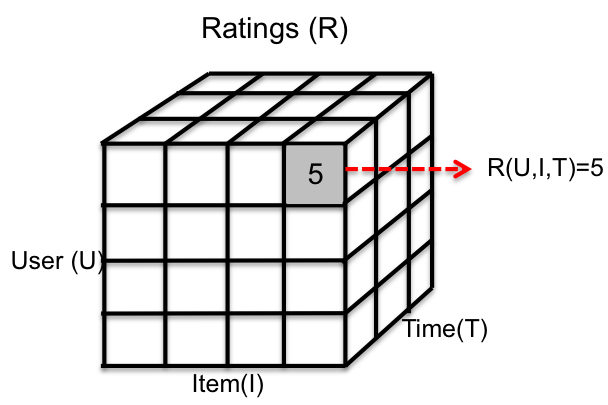
\includegraphics[width=0.40\textwidth]{img/multidimension.png}
\small
\caption{Multidimensional model of context.}
\label{fig:multidimension}   
\end{figure*}

\subsection{Paradigms for using of contextual information}

When recommender system uses contextual information, it starts
with the data having the form \textit{U * I * C * R}, where \textit{C}
is additional contextual dimension and end up with a list of
contextual recommendations $i_{1}$,$i_{2}$,$i_{3}$...$i_{n}$ for each
user. However, when the recommendation process does not take into
account  contextual information, is posible to apply the
information about the current (or desired) context \textit{c} in
various stages of the recommendation process.
Adomavicious\cite{adomavicius2011context} defines three paradigms for
the context-aware recommendation process that is based on contextual
user preference:
\begin{itemize}
\item \textbf{Contextual pre-filtering (or contextualization of
recommendation input).} The approach uses contextual information to
select the most relevant 2D (Users x Items) data for generating
recommendations. One major advantage of this approach is that it
allows deployment of any of the numerous traditional recommendation
techniques previously proposed in the literature\cite{adomavicius2005toward}.
In particular, when using this approach, context
\textit{c} essentially serves as a query (or a filter) for selecting
relevant rating data. An example of a contextual data filter for a
movie recommender system would be: if a person wants to see a movie on
Saturday, only the Saturday rating data is used to recommend movies.
Note that this example represents a crisp pre-filter because the data
was filtered using exactly the specified context (figure
\ref{fig:paradigms}.a).
\item \textbf{Contextual post-filtering (or contextualization of
recommendation output).} In this approach context information
in the input data is ignored when generating recommendations, that is, when
generating the ranked list of all candidate items from which any
number of \textit{top-N} recommendations can be made. Instead,  the
contextual post-filtering approach uses contextual information to
adjust the obtained recommendation list for each user. The
recommendation list adjustments can be made by: (1) filtering out
recommendations that are irrelevant in a given context, or (2)
adjusting the ranking of recommendations in the list. For example, in
a movie recommendation application, if a person wants to see a movie
on a weekend, and if on weekends he or she only watches comedies, the
system can filter out all noncomedies from the recommended list
(figure \ref{fig:paradigms}.b).
\item \textbf{Contextual modeling (or contextualization of
recommendation function).} This approach uses contextual information
directly in the recommendation function as an explicit predictor of a
user's rating for an item and, thus, gives rise to truly
multidimensional recommendation functions representing either
predictive models (such as decision trees, regression, and so on) or
heuristic approaches that incorporate contextual information in
addition to the user and item data (figure \ref{fig:paradigms}.c).\\
\end{itemize}
\begin{figure*}
\captionsetup{font=footnotesize}
\centering
\fbox{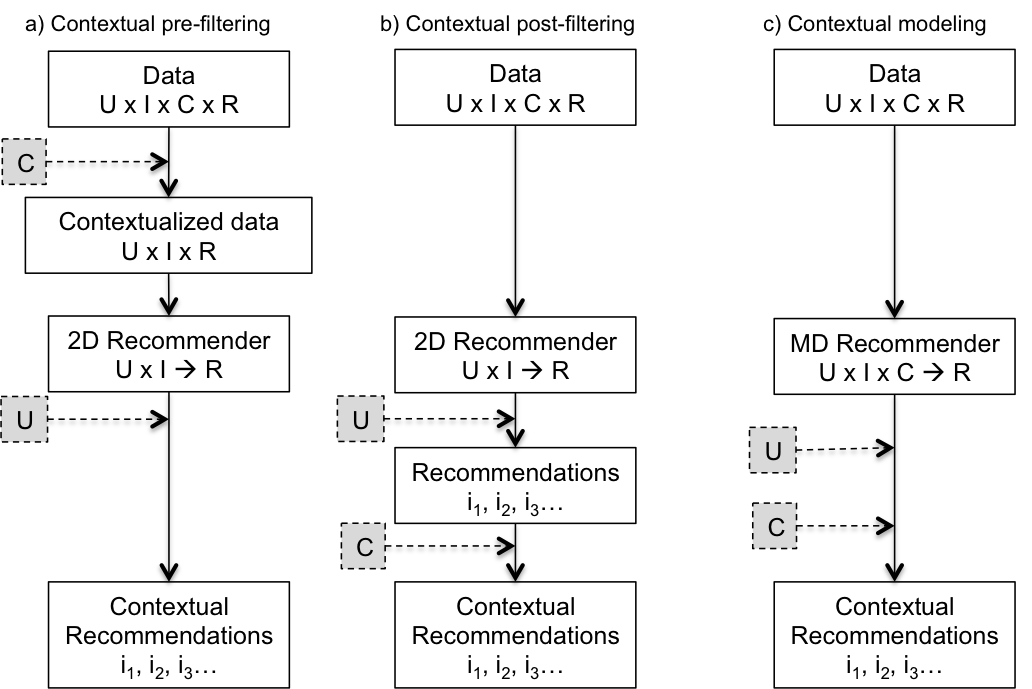
\includegraphics[width=0.80\textwidth]{img/paradigms.png}}
\small
\caption{Paradigms for incorporating context in recommender 
systems\cite{adomavicius2011context}.}
\label{fig:paradigms}   
\end{figure*}








\chapter{Proposed method}


\section{Data models} 

The data models was implemented in the DBMS with PostgreSQL database.
All the information in the context-aware recommender system was
managed in a scheme of a relational database. Each model is referring
in its section in order to have a better comprehension of each one.

\subsection{Restaurant model} 

An effective on-line recommender system must be based upon an
understanding of consumer  preferences and successfully mapping
potential products into the consumer’s
preferences\cite{adomavicius2011context}. Pan and
Fesenmaier\cite{pan2006online} argued that this can be achieved
through the understanding of how consumers describe in their own
language a product, a place, and the experience when they are
consuming the product or visiting the place.\\ Traditionally,
choosing a restaurant has been considered as rational behavior where a
number of attributes contribute to the overall usefulness of a
restaurant. For example: food type, service quality, atmosphere of the
restaurant, and availability of information about a restaurant, plays
an important role at different stages in consumer’s desitions
making\cite{auty1992consumer}. While food quality and food type have
been perceived as the most important variables for consumers’
restaurant selection, situational and contextual factors have been
found to be important also. Due to this in
Kivela\cite{jack1997restaurant} identifies 4 types of restaurants: 1)
fine dining/gourmet, 2) theme/atmosphere, 3) family/popular, and 4)
convenience/fast-food; and Auty\cite{auty1992consumer} identifies 4
types of dining out occasions: 1) namely celebration, 2) social
occasion, 3) convenience/quick meal, and 4) business meal.\\
Taking in account the context, the restaurant model proposed for
context-aware recommender system was definded with 55 attributes about the
restaurants features. An exploration about contents of models of
others works were compared to define the suitable information into the
model. Therefore, the restaurant model is a binary vector with the
following contextual attributes: 1) price range, 2) payment type, 3) alcohol
type, 4) smoking area, 5) dress code, 6) parking type, 7)
installations type, 8) atmosphere type, and 9) cuisine type. An
example of restaurant model in the context-aware recommender system is depicted in figure
\ref{fig:restaurantmodel} with some domain values of the context
represented by a binary vector where 1 means that the restaurant has
the property that corresponds to the position value. Additionally, the
restaurant model contains contextual information such as users's reviews, ratings average, and geographycal location.\\  
\begin{figure*}
\captionsetup{justification=centering,margin=2cm}
\centering
\setlength\fboxsep{0pt}
\setlength\fboxrule{0.7pt}
\fbox{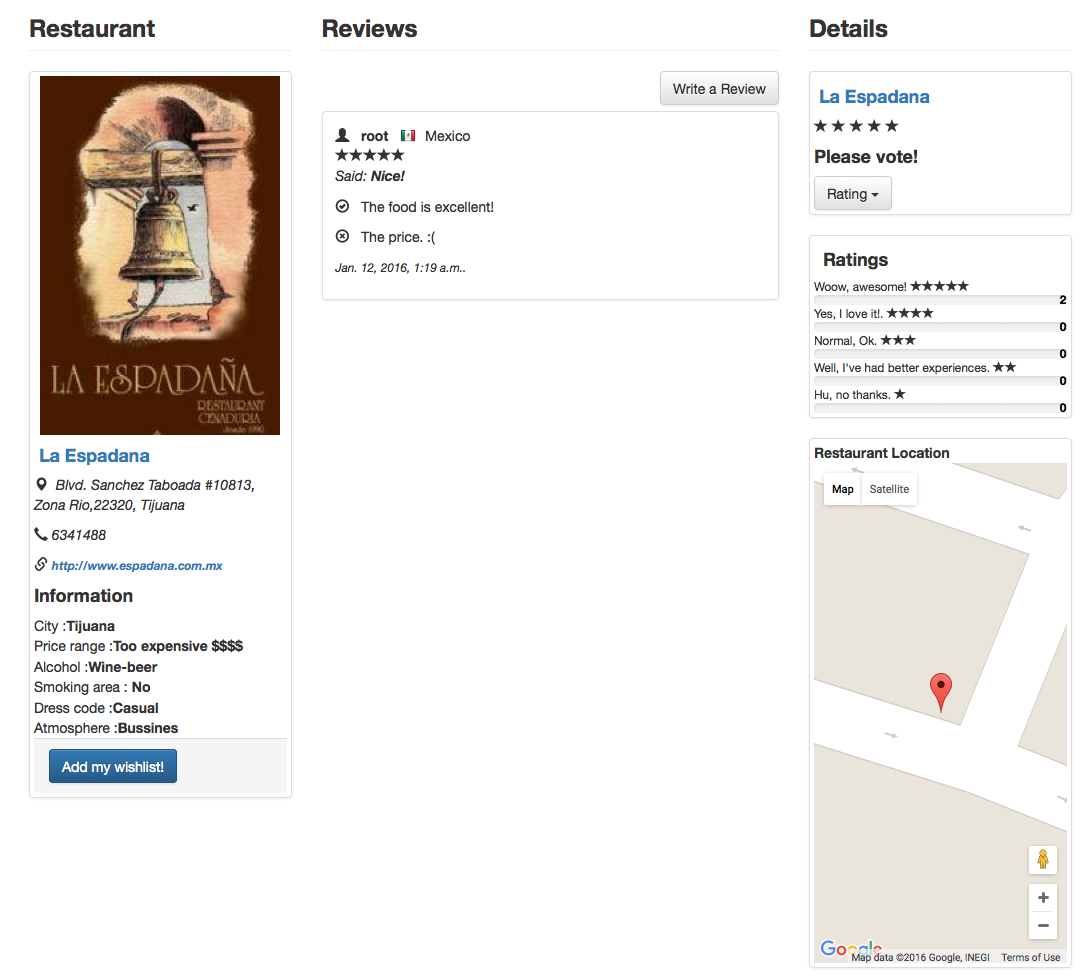
\includegraphics[width=10cm,height=10cm,keepaspectratio]{img/restaurant-model.png}}
\caption{User interface of the restaurant model.}
\label{fig:restaurantmodel}       
\end{figure*}
\subsubsection{Data model} \label{datamodelsection}   
The data model in postgreSQL is depicted in the figure
\ref{fig:restaurantmodeldata}, the model contains the restaurant
entity and its attributes. The restaurant entity is related to
\textit{Item entity} in a \textit{"one-to-one"} relation that at the
same time is related to the \textit{RecommenderRule entity} which
specifies some restrictions for item recommendations. A large view of
all the entities related is depicted in the whole scheme refered in
figure \ref{fig:datamodel}.
\begin{figure*}
\captionsetup{justification=centering,margin=2cm}
\centering
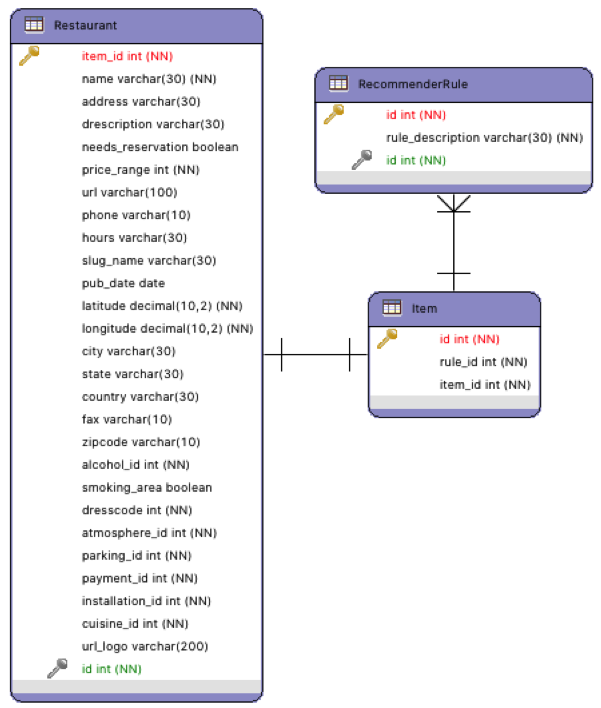
\includegraphics[width=10cm,height=10cm,keepaspectratio]{img/data-resmodel.png}
\caption{The data model of restaurant.}
\label{fig:restaurantmodeldata}     
\end{figure*}

Some related entity corresponds to the proposed catalogues, 
that are defined as following: 
\begin{itemize}
\item  \textbf{Installations:} garden, terrace, indoor, outdoor.
\item  \textbf{Atmosphere:} relax, familiar, friends, bussines, romantic.
\item  \textbf{Parking:} no parking, free parking, valet parking.
\item  \textbf{Payment:} credit/debit card, cash.
\item  \textbf{Smoking area:} yes, no.
\item  \textbf{Price:} cheap, regular, expensive, too expensive.
\item  \textbf{Dresscode:} casual, informal, formal.
\item  \textbf{Alcohol:}no alcohol, wine-beer.
\item  textbf{Cuisine:} japanese, chinese, italian, argentinean,
cantonese, mandarin, mongolian, arabic, greek, spanish, brasilian,
swiss, szechuan, asian, international, steak grill,vegetarian,
natural/healthy/light, traditional mexican, tacos, mediterranean,
middle eastern, american/fast food, gourmet, pizza, bar/beer, tapas
cafe/bar, french, birds, seafood.

\end{itemize}

The cuisines were defined according the food variety of restaurants in
Tijuana, there are 30 kinds of cuisines defined in the system. \\
The smoking area is the unique attribute with boolean value, it
defines if a restaurant has a smoking area into its installation.

\subsection{User model} 

The user's profile is derived from the ratings matrix. Let $U=[u_1,u_2,...u_n]$
the set of all users and $ I=[i_1,i_2,$...$i_n] $ the set of all items, if $R$
represent the ratings matrix,  an element  $R_{u,i}$ represents a user’s rating
$u \in U$  in a item $i \in I$.  The unknown ratings are denoted as $\neq $. The
matrix $R$ can be decomposed into rows vectors, the row vector is denoted as $
\overrightarrow{r_u} $=$[R_{u,1}$...$R_{u,|I|}]$ for every $u \in U$. Therefore,
each row vector represents the ratings of a particular user over the items. Also
denote a set of items rated by a certain user u is denoted as $ I_u = i \in I |
\forall  i: R_{u,i} \neq \emptyset $. This set of items rated represents the
user preferences where for each domain element $R_{u,i} \in [1-5]$ represents
the intensity of the user interest for  the item.\\  
\begin{figure*}
\captionsetup{justification=centering,margin=2cm}
\centering
\setlength\fboxsep{0pt}
%\setlength\fboxrule{0.60pt}
\fbox{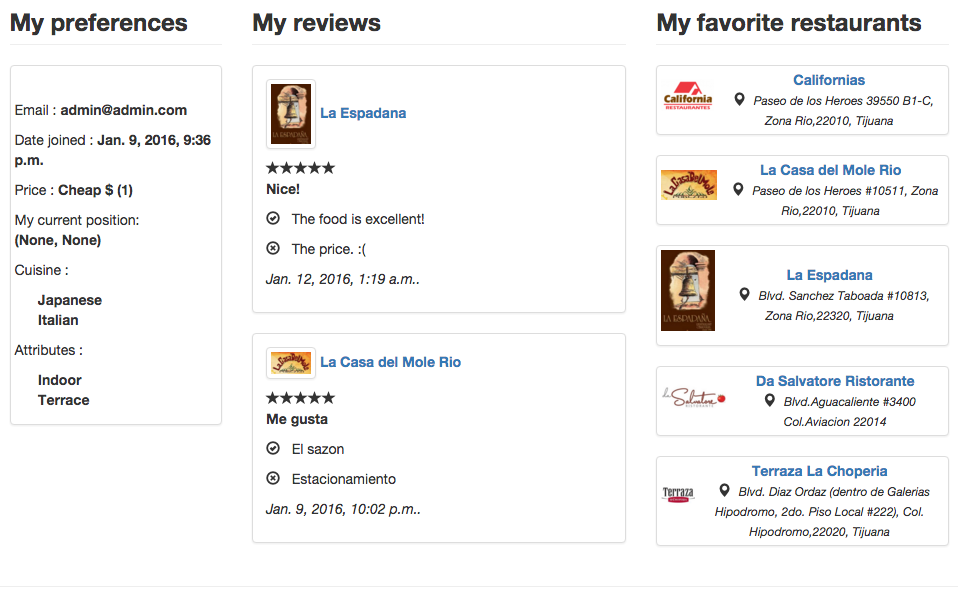
\includegraphics[width=10cm,height=10cm,keepaspectratio]{img/user-profile.png}}
\caption{Example of user interface for user profile.}
\label{fig:user-profile}       % Give a unique label
\end{figure*}
In context-aware recommender system, user profile has contextual
information such as: 1) price range, 2) current location, 3) cuisine
types, 4) attributes or features of restaurants that the user want, 5)
the reviews posted, and 6) the favorite restaurants list. The user
profile is stored in database and it is available for queries request,
and it can be changed by users many times in a session. The
information used to recommendations is the last one register stored.
The user interface is represented in figure \ref{fig:user-profile}.

\subsubsection{Data model} 

The user's data model in postgreSQL is represented in the figure
\ref{fig:datausermodel}, the model involves the entities:
\textit{User, UserProfile, and Friends.} \textit{UserProfile entity}
provides the contextual information of user, \textit{User entity} is
the default model defined in the system and is related to userProfile
for suplies valuable information. The \textit{Friends entity}
represents the social aspect into the userProfile, Friends involves
the users related to the current user taking in account the
preferences of each other. \\  The user profile entity is related with
3 catalogues: price and cuisine are the same that in restaurant model,
attribute groups corresponds to restaurant model mentioned (section
\ref{datamodelsection}). A total of 55 attributes(or features) could
be contained in user profile, this information is used such as 
contextual information also. The domain values of the related
catalogues are following:

\begin{itemize}
\item  \textbf{Price:} cheap, regular, expensive, too expensive.
\item  \textbf{Cuisine:} japanese, chinese, italian, argentinean,
cantonese, mandarin, mongolian, arabic, greek, spanish, brasilian,
swiss, szechuan, asian, international, steak grill,vegetarian,
natural/healthy/light, traditional mexican, tacos, mediterranean,
middle eastern, american/fast food, gourmet, pizza, bar/beer, tapas
cafe/bar, french, birds, seafood.
\item  \textbf{Attribute groups:} Installations, atmosphere, 
parking, payment, smoking area, dresscode, alcohol.

\end{itemize}

\begin{figure*}
%\captionsetup{justification=centering,margin=2cm}
\centering
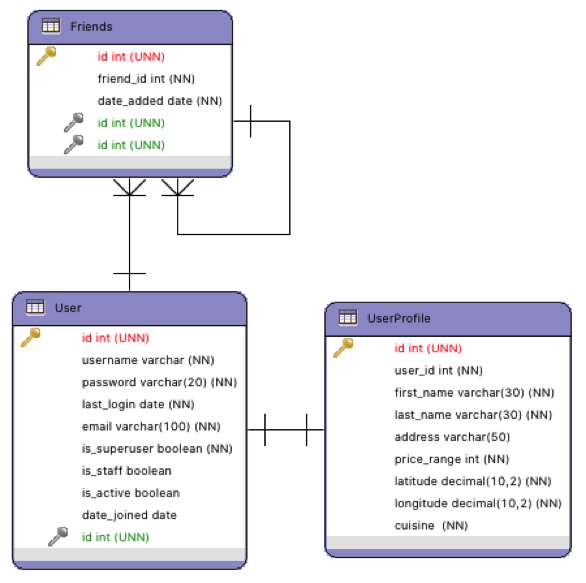
\includegraphics[width=8cm,height=8cm,keepaspectratio]{img/data-usermodel.png}
\caption{The data model of user profile.}
\label{fig:datausermodel}     
\end{figure*}

\subsection{Relational data model} 

A complete database relational scheme is represented in the figure
\ref{fig:datamodel}. This model involves the whole database for
context-aware recommender system, as well as the entities and
relations among them. \\   The context is modeled as a relational database,
each user context is a new register into data table to store user
contexts.\\  Contextual information is also stored in the entities:
\textit{Reviews, CurrentLocation, DistancePoi and Ratings.} For
instance, \textit{Reviews entity} describes the user’s opinion about
visited restaurants, this information contributes to have additional
information about recent preferences of diners.\\   
\textit{CurrentLocation entity} stores the geographical position of
user to get a \textit{"nearby recommendation"}, the system locates
restaurants around 2 kilometers from the user position. The position
is changed frequently, in this manner, it allows the adaptation for
each particular situation. \textit{Distance Poi entity} stores the
distances (kilometers) between the user and restaurants, this
information is used to calculate \textit{"nearby recommendation"}, 
each recommended restaurant ought be over the threshold defined.\\   
Finally, \textit{Rating entity} represents the user preferences 
in a vector of scores, ratings could be increased in time and 
the user's preferences patterns could be changed in time also.
\begin{landscape} 
\begin{figure}[!h] 
\centering
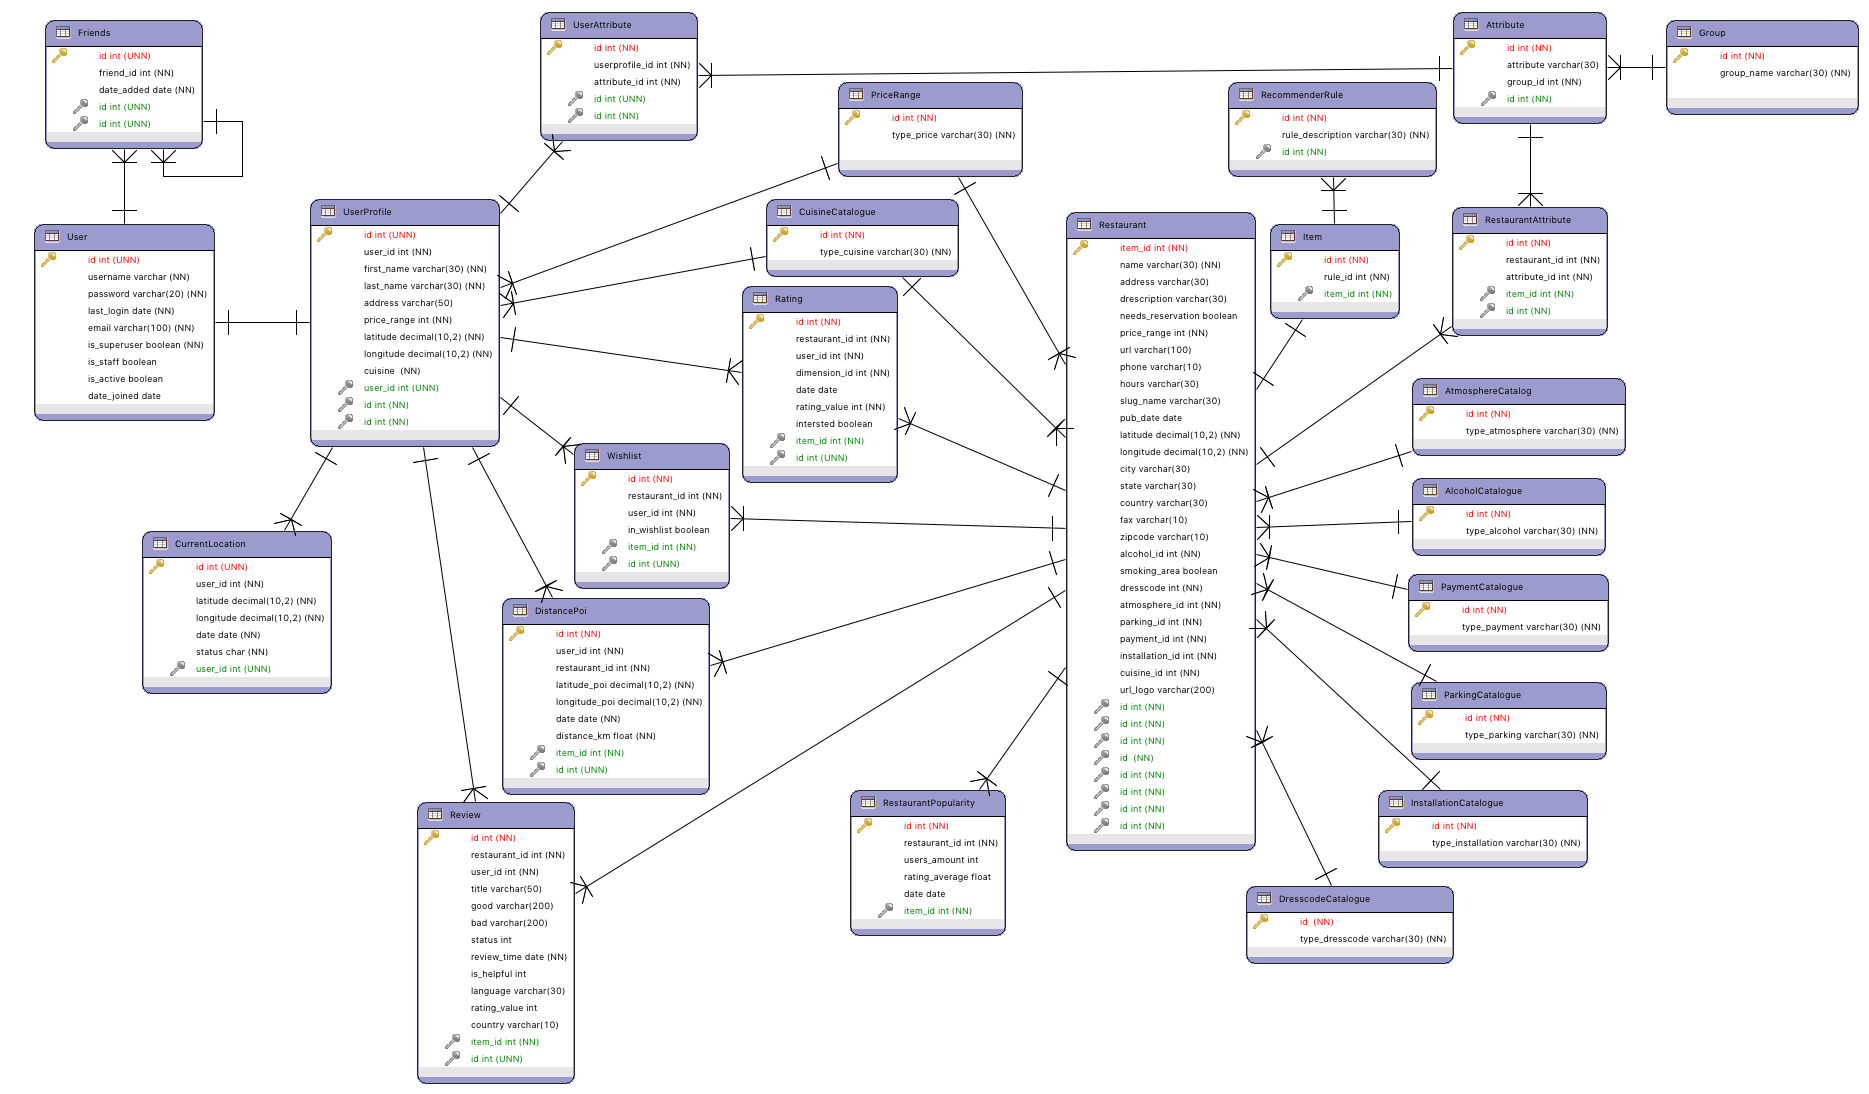
\includegraphics[width=1.3\textwidth]{img/recomet.png}
\caption{The relational database of context-aware recommender system.}
\label{fig:datamodel}    
\end{figure}
\end{landscape}

\section{Expert recomendation} 

Fuzzy logic is a methodology that provides a simple way to obtain
conclusions of linguistic data. Is based on the traditional process of
how a person makes decisions based in linguistic information. \\    Fuzzy
logic is a computational intelligence technique that allows to use
information with a high degree of inaccuracy; this is the difference
with the conventional logic that only uses concrete and accurately
information \cite{zedeh1989knowledge}.\\  In this work, fuzzy logic is
used to model fuzzy variables that highligh in the popularity of a
restaurant. The context-aware recommender system has implemented a
Fuzzy Inference System that represents the expert recommendation. \\   The
expert Fuzzy Inference System generates recommendations when the
recommendation techniques (collaborative filtering, content-based) are
not getting results because of the cold start problem.\\   The Fuzzy
Inference System proposed has 3 \textbf{input variables} (such as in
previous work realized\cite{garcia2009hybrid}): 1)\textit{rating} is
an average of ratings that has a particular restaurant inside the user
community; the domain of variable is 0 to 5 and contains 2 membership
functions labeled as \textit{low} and \textit{high}(figure
\ref{fig:mf:a}), 2)\textit{price} represents the kind of price that
has a particular restaurant; the domain of variable is 0 to 5 and
contains 2 membership functions labeled as \textit{low} and
\textit{high} (figure \ref{fig:mf:b}), and 3)\textit{votes} is used to
measure how many items have been rated by the current user, i.e., the
participation of the user, if the user has rated few items (less than
10) is not sufficient to make accurate predictions(figure
\ref{fig:mf:c}), the domain of variable is 0 to 10 and contains 2
membership functions labeled as \textit{insufficient} and
\textit{sufficient}. \\   The \textbf{output variable} is
\textit{recommendation}, represents a weight for each restaurant
proposed by the expert considering the inputs mentioned above, the
domain of variable is 0 to 5 and contains 3 membership functions
labeled as \textit{low}, \textit{medium} and \textit{high} (figure
\ref{fig:mf:d}).

\begin{figure}[ht!]
   \centering
   %%----primera subfigura----
   \subfloat[]{
        \label{fig:mf:a}
        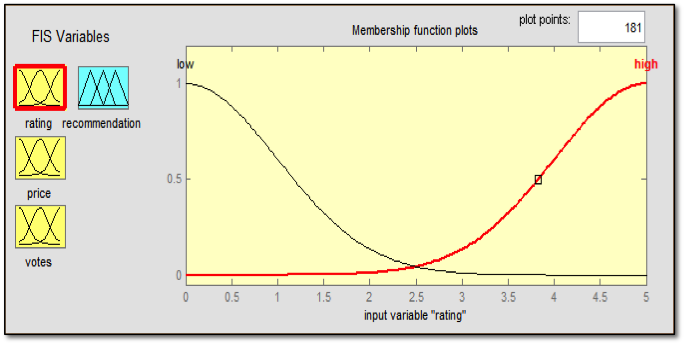
\includegraphics[width=0.42\textwidth]{img/mf-rating.png}}
   \hspace{0.1\linewidth}
   %%----segunda subfigura----
   \subfloat[]{
        \label{fig:mf:b} 
        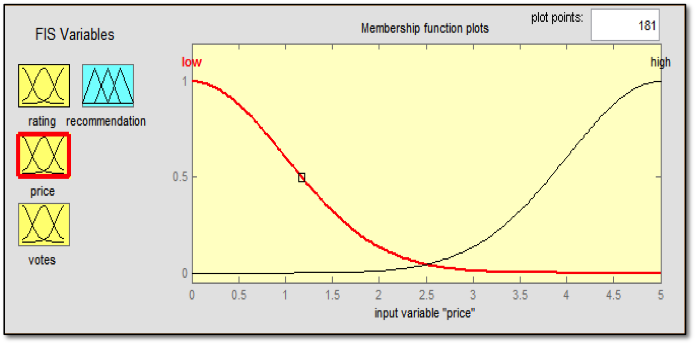
\includegraphics[width=0.42\textwidth]{img/mf-price.png}}\\[20pt]
   %%----tercera subfigura----
   \subfloat[]{
        \label{fig:mf:c} 
        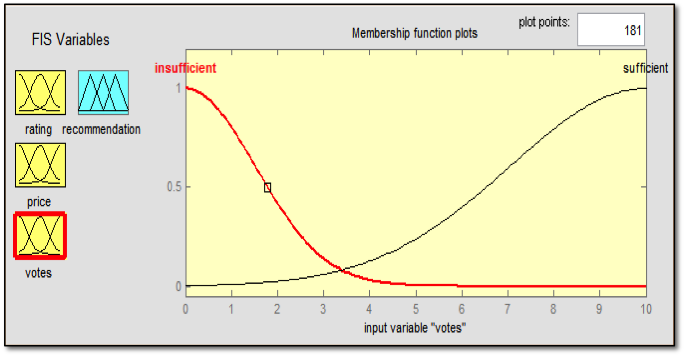
\includegraphics[width=0.42\textwidth]{img/mf-votes.png}}
    \hspace{0.1\linewidth}
   %%----cuarta subfigura----
    \subfloat[]{
        \label{fig:mf:d} 
        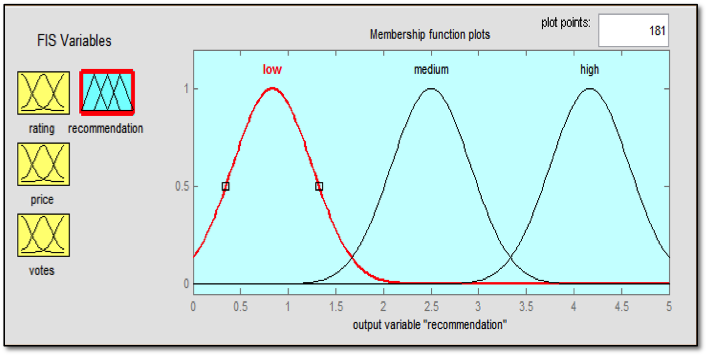
\includegraphics[width=0.42\textwidth]{img/mf-recommendation.png}}
   \caption{The Gaussian membership functions of the expert system.
   }
   \label{fig:mfexpert} 
\end{figure}

The proposed Fuzzy Inference System(figure \ref{fig:expertfis})
represents the users experience and their knowledge about restaurants.
This factors are considered important  for users that visiting a
restaurant. This information is recovered of user profile and
restaurant profile; and the system uses this information to get
weights that influence in the final recommendations. The Fuzzy
Inference System uses 5 inference rules that involve the variables of
inputs and output.The input variables determine the recommendation
activation; each input variable contains labels as \textit{low} and
\textit{high} that also correspond to memberships functions of
Gaussian type. For the output variable \textit{recommendation} the
labels \textit{low}, \textit{medium}, and \textit{high} are used with
membership functions Gaussian type also. The rules are:
\begin{enumerate} 
\item \textit{If \textbf{rating} is high and \textbf{price} is low then \textbf{recommendation} is high.}
\item \textit{If \textbf{rating} is high and \textbf{votes} is sufficient then \textbf{recommendation} is high.}
\item \textit{If \textbf{rating} is high and \textbf{votes} is insufficient then \textbf{recommendation} is medium.}
\item \textit{If \textbf{rating} is low and \textbf{price} is high and then \textbf{recommendation} is low.} 
\item \textit{If \textbf{rating} is low and \textbf{votes} is insufficient then \textbf{recommendation} is low.}
\end{enumerate} 
\begin{figure*}
\captionsetup{justification=centering,margin=2cm}
\centering
\fbox{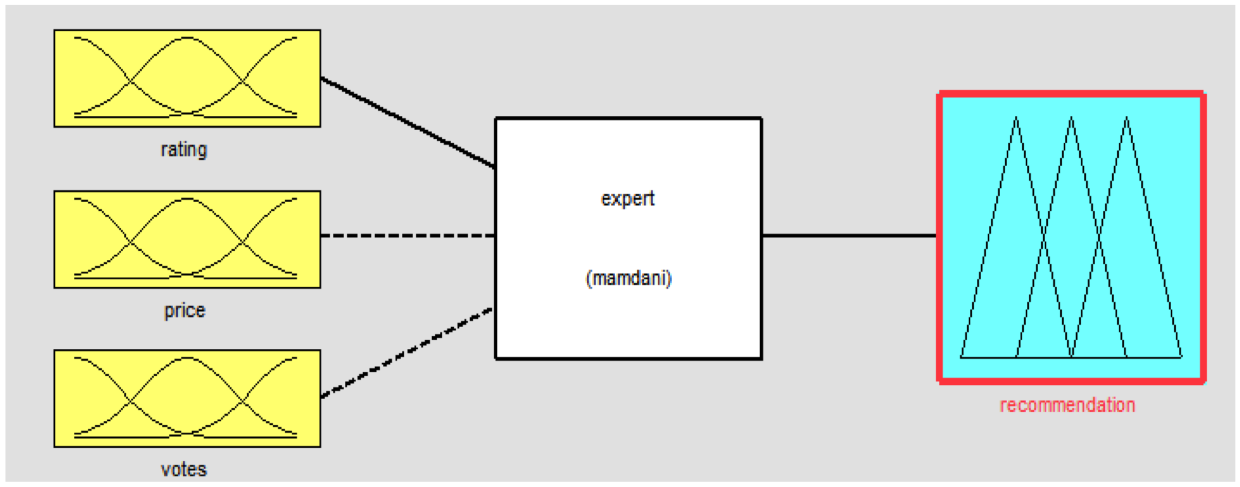
\includegraphics[width=0.70\textwidth]{img/expert.png}}
\caption{Fuzzy Inference System of expert.}
\label{fig:expertfis}       % Give a unique label
\end{figure*}

\section{Fuzzy Inference System to assing weights} 

The main goal of this Fuzzy Inference System is to define weights for each recommendation list. The recommendation technique is based in the amount of available information stored, so each technique utilizes this information to provide a list of restaurants as well as a weight for each one, therefore, these is used for  recommendations if its weight is upper the threshold.  The Fuzzy Inference System has inputs and outputs to infer each list's weight, its variables are depicted in figure \ref{fig:fis-pesos}. 
There are 3 membership functions for inputs and 3 for outputs. The input variables are: \textit{userSimilarity, restaurantSimilarity and Participation} and are depicted in figure \ref{fig:fis-inputs}. The (\ref{fig:fis-inputs}.a) and(\ref{fig:fis-inputs}.b) are in a range from 0 to 1 to define the similarity average among users and restaurants, respectively. The figure (\ref{fig:fis-inputs}.c) has a range from 0 to 15  to represent the ratings of the user(participation). This information is stored in the Popularity entity (see figure \ref{fig:datamodel}). \\
\begin{figure*}
\captionsetup{justification=centering,margin=2cm}
\centering
\fbox{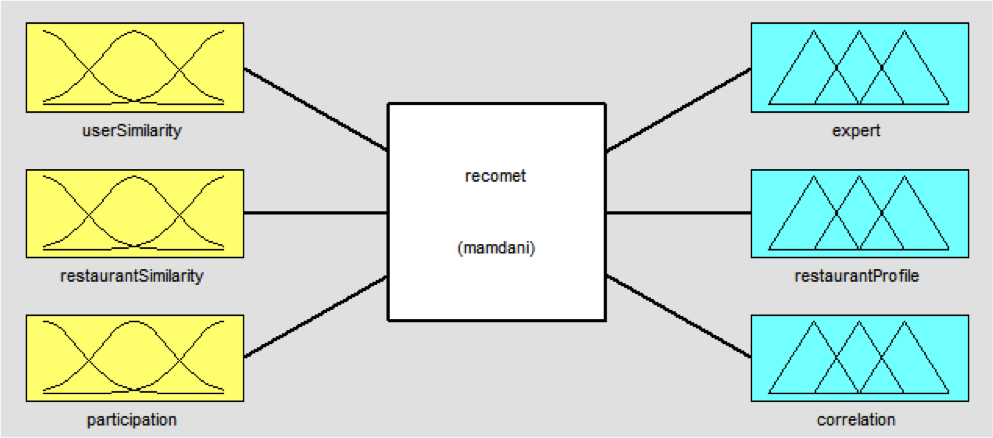
\includegraphics[width=0.70\textwidth]{img/fis-pesos.png}}
\caption{Fuzzy Inference System to assign weights.}
\label{fig:fis-pesos}       % Give a unique label
\end{figure*}
By other side, the output variables are: \textit{Expert, RestaurantProfile and Correlation}, these are depicted in figure \ref{fig:fis-outputs}. The figure (\ref{fig:fis-outputs}.a) represents the weight for expert recommendation list, figure (\ref{fig:fis-outputs}.b) represents the weight of the content-based list and figure (\ref{fig:fis-outputs}.c) represents the weight of collaborative recommendation list, their membership functions are in a range from 0 to 1 to get the value.
\begin{figure}[ht!]
   \centering
   %----primera subfigura----
   \subfloat[]{
        \label{fig:mf:a}
        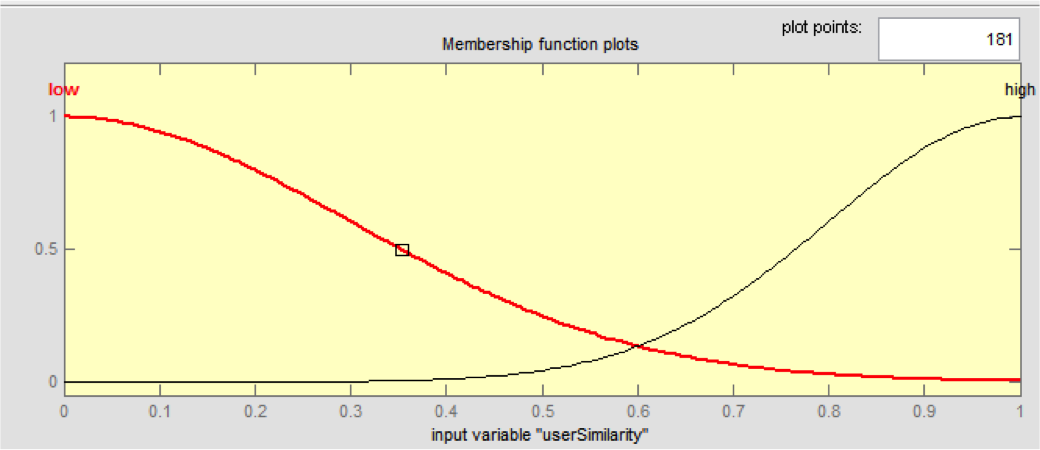
\includegraphics[width=0.42\textwidth]{img/usersimilarity.png}}
   \hspace{0.1\linewidth}
   %%----segunda subfigura----
   \subfloat[]{
        \label{fig:mf:b} 
        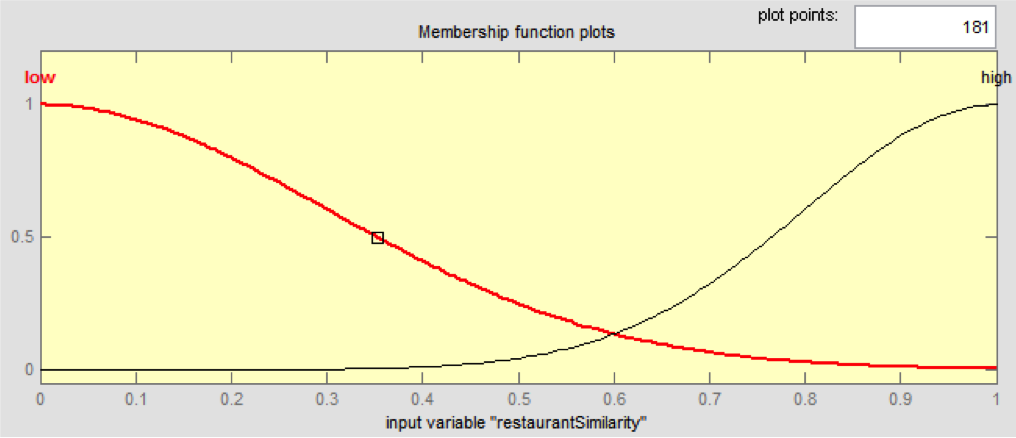
\includegraphics[width=0.42\textwidth]{img/restaurantsimilarity.png}}\\% [20pt]
   %%----tercera subfigura----
   \subfloat[]{
        \label{fig:mf:c} 
        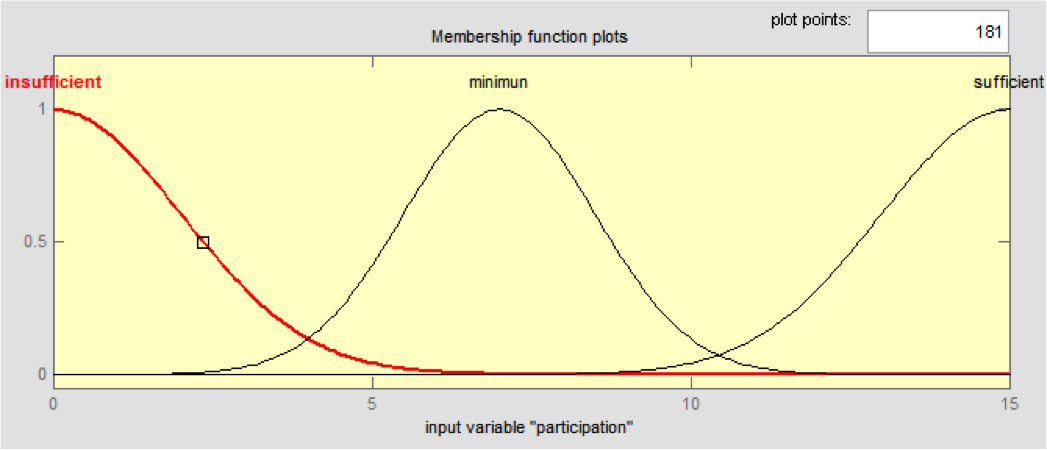
\includegraphics[width=0.42\textwidth]{img/participation.png}}
        %\hspace{0.1\linewidth}
   \caption{The Gaussian membership functions of input variables.
   }
   \label{fig:fis-inputs} 
\end{figure}
\begin{figure}[ht!]
   \centering
   %%----primera subfigura----
    \subfloat[]{
        \label{fig:mf:d} 
        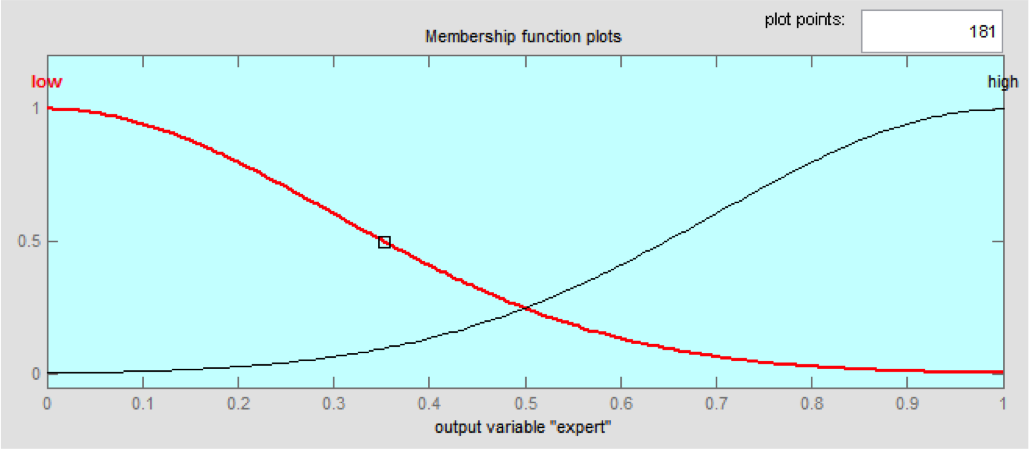
\includegraphics[width=0.42\textwidth]{img/expert-mf.png}}%\\ %[20pt]
        \hspace{0.1\linewidth}
      %%----segunda subfigura----
    \subfloat[]{
        \label{fig:mf:d} 
        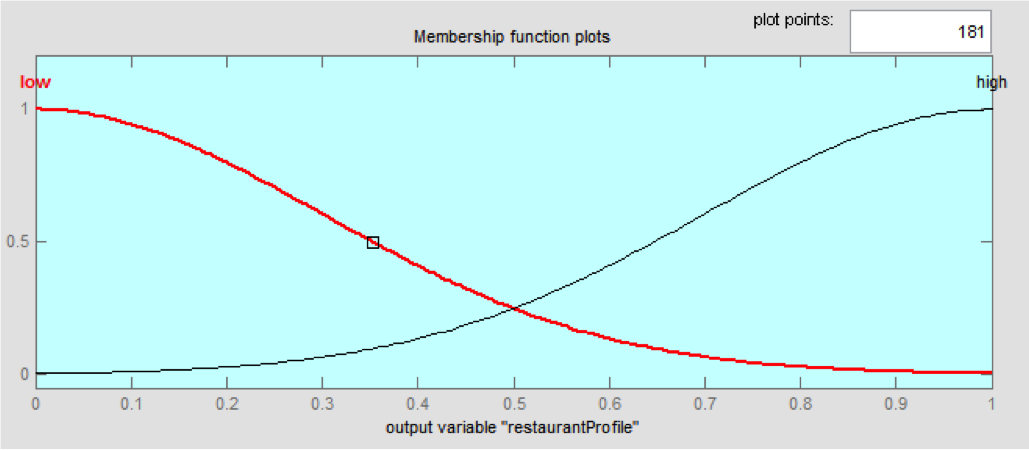
\includegraphics[width=0.42\textwidth]{img/restaurantprofile-mf.png}}\\
     %%----tercera subfigura----
    \subfloat[]{
        \label{fig:mf:d} 
        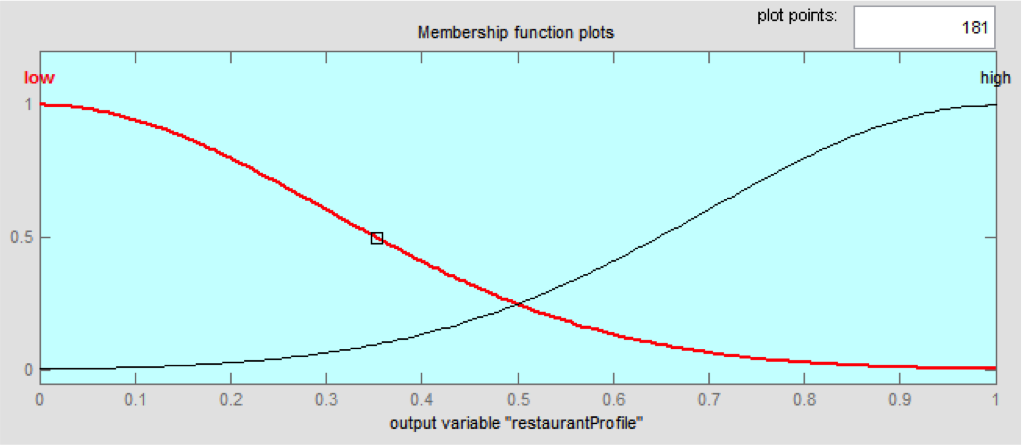
\includegraphics[width=0.42\textwidth]{img/correlation-mf.png}}%\\ %[20pt]
   \caption{The Gaussian membership functions of output variables.
   }
   \label{fig:fis-outputs} 
\end{figure}
Taking in account the input variables, the rules utilized to infer the 
output values are following:
\begin{enumerate} 
\item \textit{If \textbf{userSimilarity} is low and 
\textbf{restaurantSimilarity} is low and \textbf{participation} 
is insufficient then \textbf{expert} is high, \textbf{restaurantProfile} 
is low, \textbf{correlation} is low.}
\item \textit{If \textbf{userSimilarity} is low and 
\textbf{restaurantSimilarity} is low and \textbf{participation} 
is sufficient then \textbf{expert} is low, \textbf{restaurantProfile} 
is low, \textbf{correlation} is high.}
\item \textit{If \textbf{userSimilarity} is low and 
\textbf{restaurantSimilarity} is low and \textbf{participation} 
is minimun then \textbf{expert} is low, \textbf{restaurantProfile} 
is low, \textbf{correlation} is high.}
\item \textit{If \textbf{userSimilarity} is low and 
\textbf{restaurantSimilarity} is high and \textbf{participation} 
is insufficient then \textbf{expert} is low, \textbf{restaurantProfile} 
is high, \textbf{correlation} is low.}
\item \textit{If \textbf{userSimilarity} is low and 
\textbf{restaurantSimilarity} is high and \textbf{participation} 
is minimun then \textbf{expert} is low, \textbf{restaurantProfile} i
s high, \textbf{correlation} is low.}
\item \textit{If \textbf{userSimilarity} is low and 
\textbf{restaurantSimilarity} is high and \textbf{participation} 
is sufficient then \textbf{expert} is low, \textbf{restaurantProfile} 
is high, \textbf{correlation} is low.}
\item \textit{If \textbf{userSimilarity} is high and 
\textbf{restaurantSimilarity} is low and \textbf{participation} 
is insufficient then \textbf{expert} is low, \textbf{restaurantProfile} 
is low, \textbf{correlation} is high.}
\item \textit{If \textbf{userSimilarity} is high and 
\textbf{restaurantSimilarity} is low and \textbf{participation} 
is minimun then \textbf{expert} is low, \textbf{restaurantProfile} 
is low, \textbf{correlation} is high.}
\item \textit{If \textbf{userSimilarity} is high and 
\textbf{restaurantSimilarity} is low and \textbf{participation} 
is sufficient then \textbf{expert} is low, \textbf{restaurantProfile} 
is low, \textbf{correlation} is high.}
\item \textit{If \textbf{userSimilarity} is high and 
\textbf{restaurantSimilarity} is high and \textbf{participation} 
is insufficient then \textbf{expert} is low, \textbf{restaurantProfile} 
is low, \textbf{correlation} is high.}
\item \textit{If \textbf{userSimilarity} is high and 
\textbf{restaurantSimilarity} is high and \textbf{participation} 
is sufficient then \textbf{expert} is low, \textbf{restaurantProfile} 
is low, \textbf{correlation} is high.}
\item \textit{If \textbf{userSimilarity} is high and 
\textbf{restaurantSimilarity} is high and \textbf{participation} 
is minimun then \textbf{expert} is low, \textbf{restaurantProfile} 
is low, \textbf{correlation} is high.}
\end{enumerate} 

\section{Contextual Recommendation} 

The interface of the system(figure \ref{fig:context})  allows to
collect contextual information such as type of price, restaurant's
attributes, type of cuisine and geographical location.  The context-
aware recommender system uses pre-filtering paradigm, then the
contextual information is used for adjust the final recommendations
list.  For example, geographical location is used to get restaurants
around  2 kilometers of distance, next, the list of nearby restaurants
is displayed  for the user. If context-aware recommender system
considers another  attributes as type of price and type of cuisine
preferred by the user, the system gets restaurants matched in the
context especified  by the user in this time.  In the attributes box,
the user can chose any preference about what things are importants to
select a restaurant. The features are collected from the dataset of
Tijuana restaurants. In the cuisine box, the user choosen his/her
favorite cuisine, it can be one or more cuisines such as in attributes also. \\  
The context changes constantly, indeed, the users migh change 
it many times such as them wish.
\begin{figure*}
\captionsetup{justification=centering,margin=2cm}
\centering
\fbox{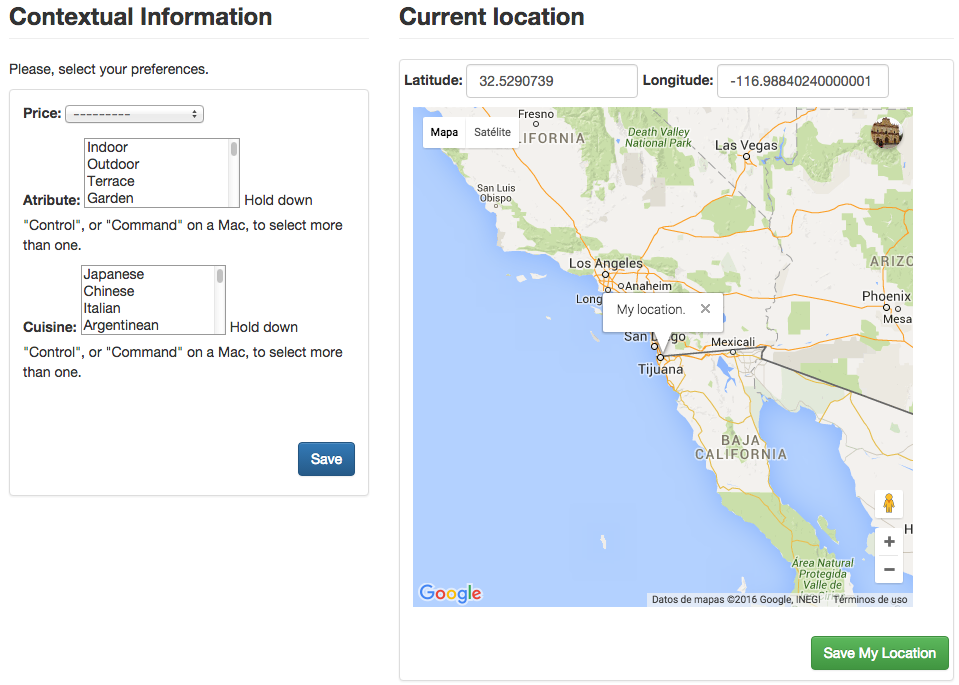
\includegraphics[width=0.60\textwidth]{img/context.png}}
\caption{System interface to collect contextual information.}
\label{fig:context}   
\end{figure*}
After the post-filtering, the system displays the  recommended
restaurants according the information provides by the user. The
context-aware recommender system contains 4 techniques to display
recommendations. The interface in figure \ref{fig:recom} shows
recommendations: \textit{1) Expert, 2) Content- based, 3) Collaborative
filtering and 4) Nearby.} Each one was explained above, except the
nearby recommendations. For nearby recommendations the system
calculates the approximate distance between the current geographical
location of the user and the available restaurants in the area.  The
threshold is 2 kilometers around the user position to determine what
restaurants will be recommended.  The geographical position is
obtained throught Google maps.

\begin{figure*}
%\captionsetup{justification=centering,margin=2cm}
\centering
\fbox{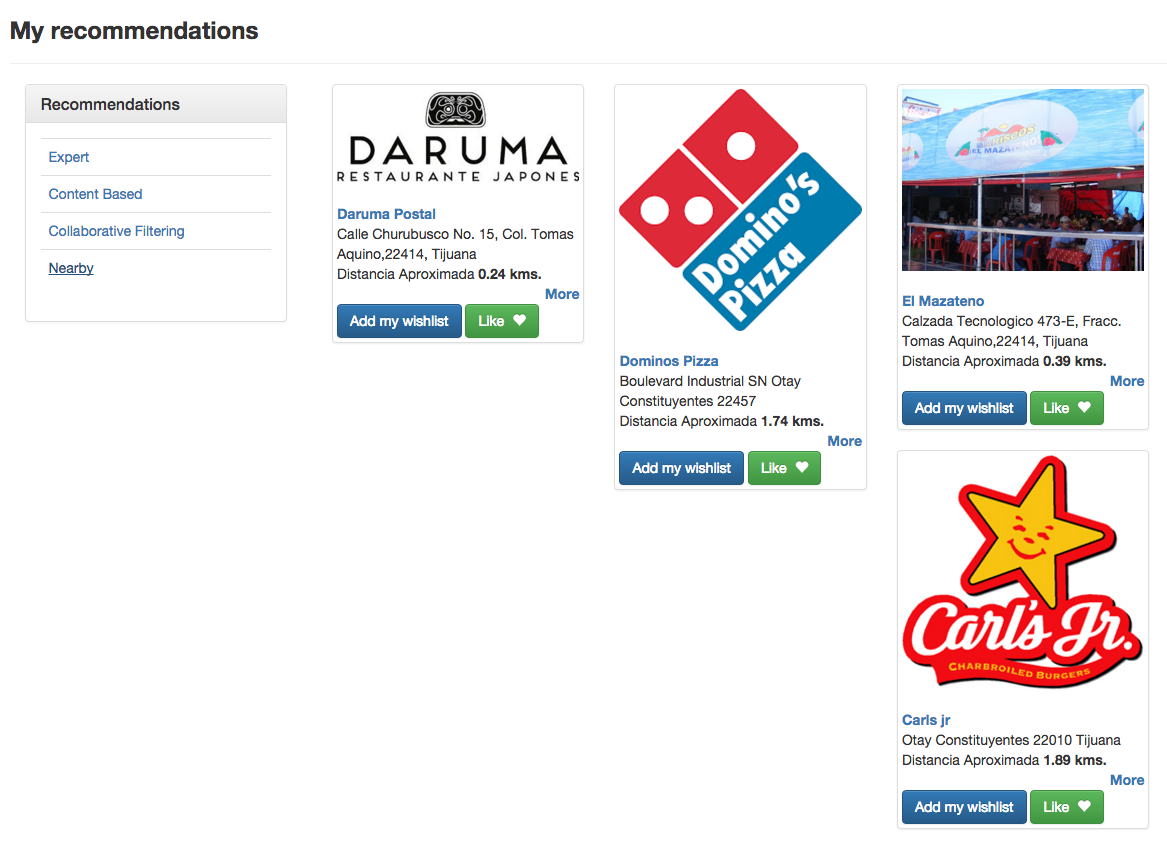
\includegraphics[width=0.60\textwidth]{img/recom.png}}
\caption{System inferface of recommendations for the user.}
\label{fig:recom}    
\end{figure*}

\section{Methodology} 

The scheme of poposed method is depicted in the figure
\ref{fig:archit}.  In the first part, the three techniques of
recommendations are suplied by the rating matrix to obtain the
recommendation list. Ratings matrix makes that Fuzzy Inference System
can obtain the inputs values to calculate the output value. The
Content-based utilizes the rating matrix and user profiles to compare
the similarity among the restaurants through cosine similarity. The
collaborative filtering is based in rating matrix (user profiles) to
predict ratings for restaurants using Pearson correlation to get the K
neighbors.\\ 
The second part shows the recommendation lists for the user getting of
each algorithm. Subsequently, the recommendation lists are reduced
when filter context is applied, i.e., the recommendations are adjusted
for the user current context. Finally, the contextual recommendations
list is displayed in the user interface (figure \ref{fig:recom}).
\begin{figure*}
%\captionsetup{justification=centering,margin=2cm}
\centering 
\fbox{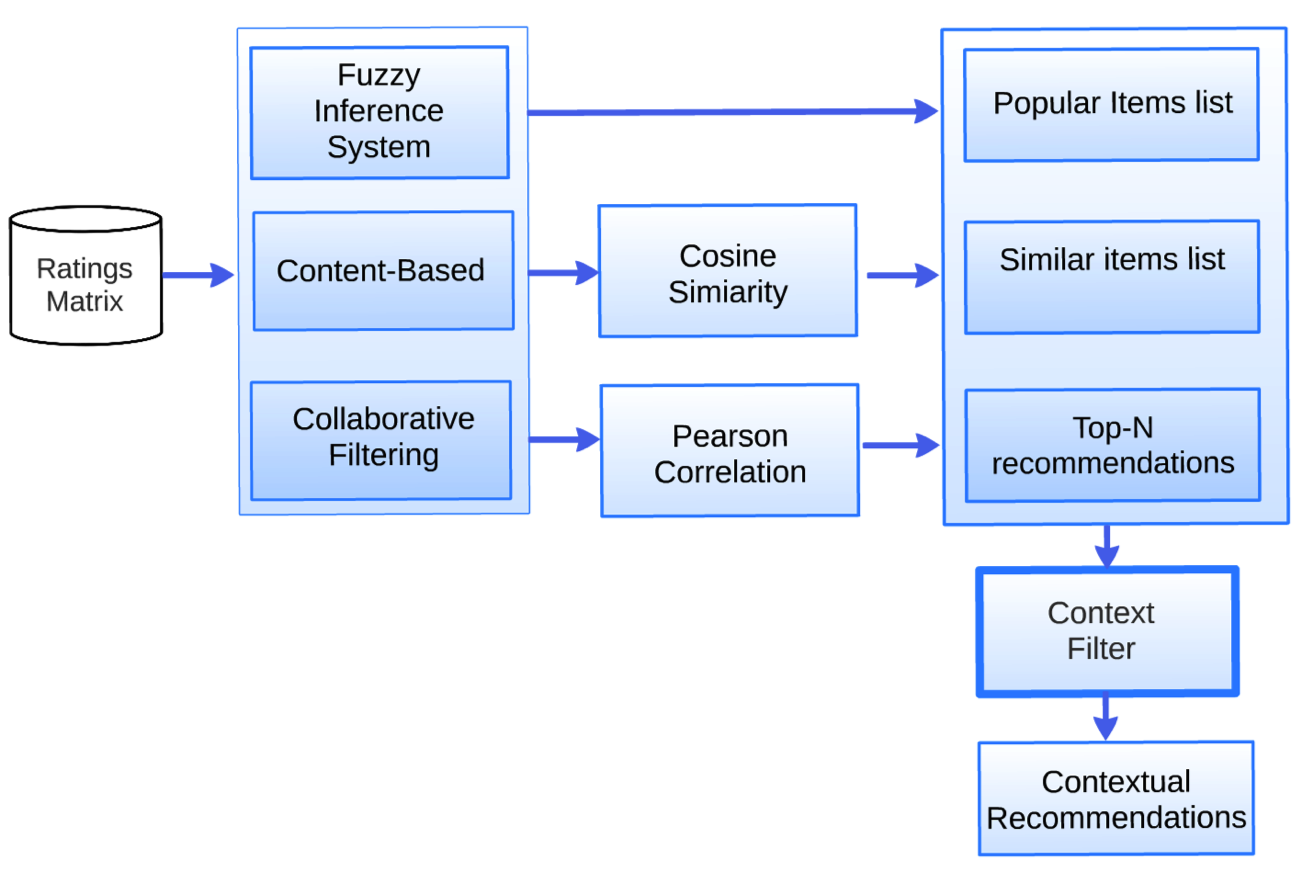
\includegraphics[width=10cm,height=10cm,keepaspectratio]{img/archit.png}}
%\fbox{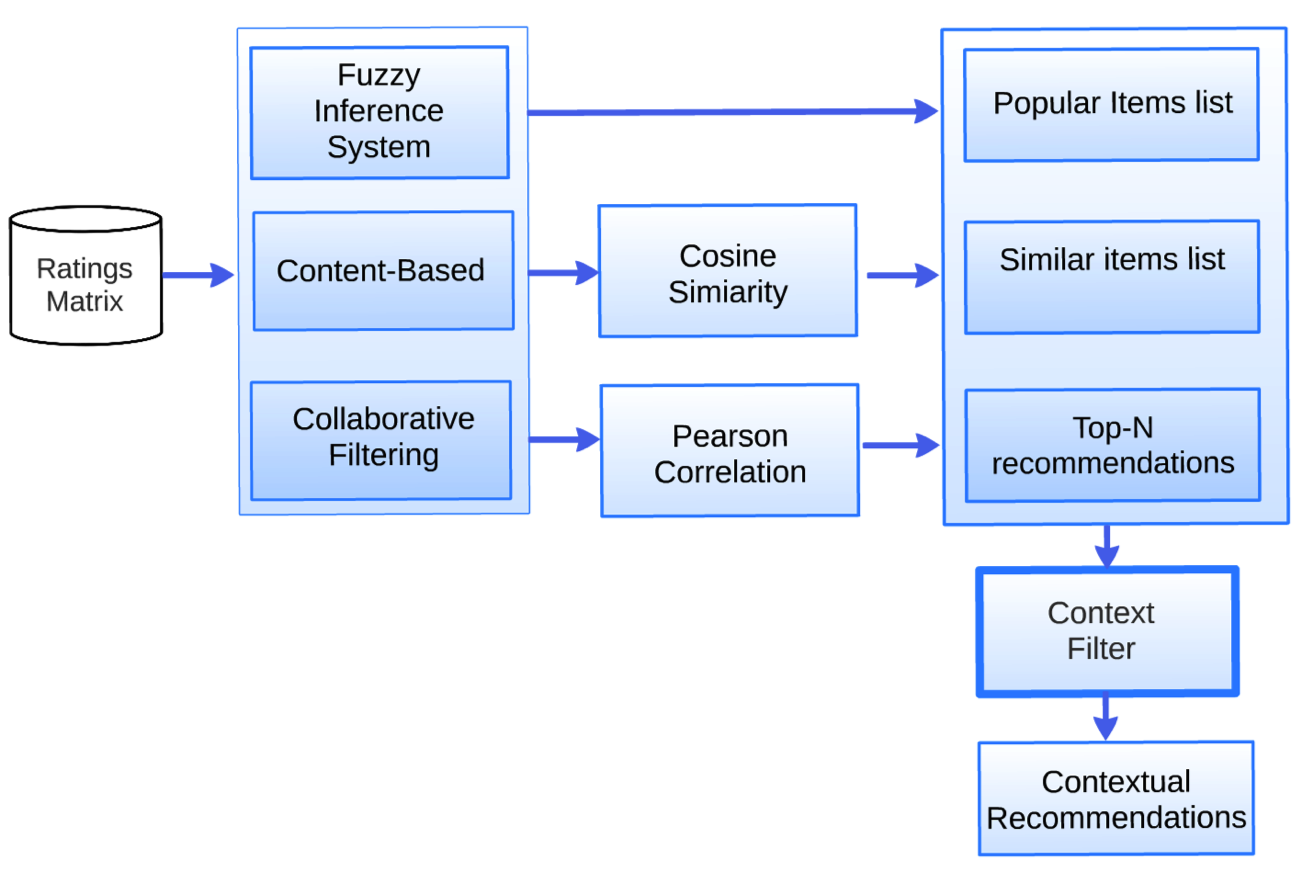
\includegraphics[width=0.60\textwidth]{img/archit.png}}
\caption{Context-aware recommender system methodology.}
\label{fig:archit}       % Give a unique label
\end{figure*}






\chapter{Case of study} \label{case}

<<<<<<< HEAD
In this chapter we present the relevant experiments that were done to
test the proposed method. Subsequently, it shows the implementation of
the method in a restaurant recommender system used as case of study, 
the context was integrated into the recommender system when   
we consider the contextual factors. A wide explanation of the system  
interfaces and its functionality is explained also.

\section{Experimental settings} 

In this particular experimental scenario, the basic guidelines 
proposed in Adomavicius  \cite{adomavicius2011context} are followed,  
=======
\section{Experimental settings} 

In this particular experimental scenario, the basic guidelines 
proposed in Adomavicius \cite{adomavicius2011context} are followed,  
>>>>>>> origin/master
and they are briefly explained next. 
\begin{itemize} 
\item \textbf{Hypothesis:} before running the experiment we must form
an \textit{hypothesis}. It is important to be concise and restrictive
about this hypothesis, and design an experiment that tests the
<<<<<<< HEAD
hypothesis. For example, an hypothesis can be that  \textit{algorithm
A} predicts better user ratings than  \textit{algorithm B}.  In that
=======
hypothesis. For example, an hypothesis can be that  \textbf{algorithm
A} predicts better user ratings than  \textbf{algorithm B}.  In that
>>>>>>> origin/master
case, the experiment should test the prediction accuracy, and not
other factors.
\item \textbf{Controlling variables:} when comparing a few candidate
algorithms on a certain hypothesis, it is important that all
\textit{variables} that are not tested will stay fixed. For example,
suppose that we wish to compare the prediction accuracy of movie
<<<<<<< HEAD
ratings of  \textit{algorithm A} and \textit{algorithm B}, that both
=======
ratings of  \textbf{algorithm A} and \textbf{algorithm B}, that both
>>>>>>> origin/master
use different collaborative filtering models.
\item \textbf{Generalization power:} when drawing conclusions from
experiments, we may desire that our conclusions generalize beyond the
immediate context of the experiments. When choosing an algorithm for a
real application, we may want our conclusions to hold on the deployed
system, and generalize beyond our experimental data set. Similarly,
when developing new algorithms, we want our conclusions to hold beyond
the scope of the specific application or data set that we experimented
with. It is important to understand the properties of the various data
sets that are used. Generally speaking, \textit{the more diverse the
data used, the more it can generalize the results}.
\end{itemize} 

\subsection{Off-line experiments} 

An off-line experiment is performed using a pre-collected dataset
of users' selections or ratings. By using this dataset we try to simulate
<<<<<<< HEAD
the behavior of users that will interact with the recommender system. \\In
=======
the behavior of users that will interact with the recommender system. In
>>>>>>> origin/master
doing so, it is assumed that the user behavior when the data was collected
will be similar enough to the users' behavior when the recommender
system is deployed, so that we can make reliable decisions based on
the simulation.  Off-line experiments are attractive because they
\textit{require no interaction with real users}, and thus it allows to compare
a wide range of candidate algorithms at a low cost. \\ The downside is
that it can answer a very narrow set of questions, typically questions
about the prediction of an algorithm. The goal of the off-line
experiments is to filter out inappropriate  approaches, leaving a
relatively small set of alternatives algorithms for subsequently to be
tested for the more costly user studies or on-line 
<<<<<<< HEAD
experiments  \cite{adomavicius2011context}.\\
The next sections show a comprehensive description of the 
experimental setup for experiments, as well as results obtained 
in the experiments. Each method was tested using contextual 
datasets in the domain.  This chapter ends with the  
description of the functionality of the prototype used to 
validate the method utilized in the experiments.

\section{Restaurants recommendations} \label{restaurants}

=======
experiments\cite{adomavicius2011context}.\\ 

The next sections show a comprehensive description of the 
experimental setup for experiments, as well as results obtained 
in the experiments. Each method was tested using contextual 
datasets in the domain.  This chapter ends with the entire 
description of the functionality of the prototype used to 
validate the method utilized in the experiments.

\section{Restaurants recommendations} \label{restaurants}.
>>>>>>> origin/master
In earlier implementations of the context-aware recommender system  
several experiments were cundunted to test the behaviour of algorithms 
and the performance in the proposed methods. 
For the experiment the proposed hypothesis is \textit{The accuracy of 
recommendations is improved using context factors in the 
<<<<<<< HEAD
recommendation process}. 
\begin{figure*}
\centering
\captionsetup{font=footnotesize}
\setlength\fboxsep{0pt}
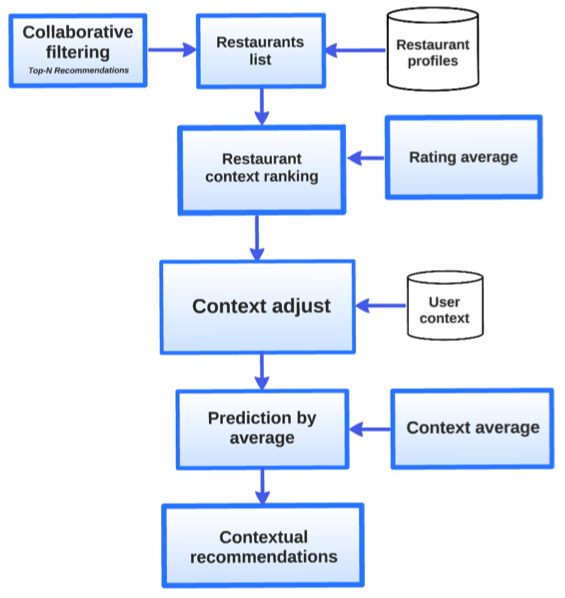
\includegraphics[width=0.50\textwidth]{img/posfil.png}
\caption{The post-filtering approach for Tijuana restaurants.}
\label{fig:postfiltering}     
\end{figure*}
To validate the hypothesis the next test was realized.
A first experiment described in  \cite{ramirez2013restaurant}, presents a  
contextual recommender system using the post-filtering approach and 
collaborative filtering technique in a restaurant domain. 
Collaborative filtering works to get a Top-N list utilized to adjust it in 
the context. \\
=======
recommendation process}. To validate the hypothesis the next test  
was realized. \\
A first experiment described in \cite{ramirez2013restaurant} and presents a  
contextual recommender system using the post-filtering approach and 
collaborative filtering technique in a restaurant domain. 
Collaborative filtering works to get a Top-N list utilized to adjust it in 
the context. 
>>>>>>> origin/master
Later, the Top-N list is obtained and the restaurants are adjusted to 
make ranking of restaurants  in the current context. Post-filtering is
based on the average  of ratings in a specific context, so prediction
is made with: 1) \textit{the average} that a restaurant has in the
<<<<<<< HEAD
current context (that is the  mean of user ratings) and 2)  
 \textit{the rating} predicted by the collaborative filtering algorithm.\\ 
Top-N list contains the restaurants with highest predictions, 
so each restaurant is adjusted for the user's context and listed in 
contextual recommendations; the process is depicted in 
Figure  \ref{fig:postfiltering}.
=======
current context (that is the  mean of user ratings) and 2) 
\textit{the rating} predicted by the collaborative filtering algorithm. 
The top-N list contains the restaurants with highest predictions, 
so each restaurant is adjusted for the user's context and listed in 
contextual recommendations; the process is depicted in figure
\ref{fig:postfiltering}.
\begin{figure*}
\centering
\captionsetup{font=footnotesize}
\setlength\fboxsep{0pt}
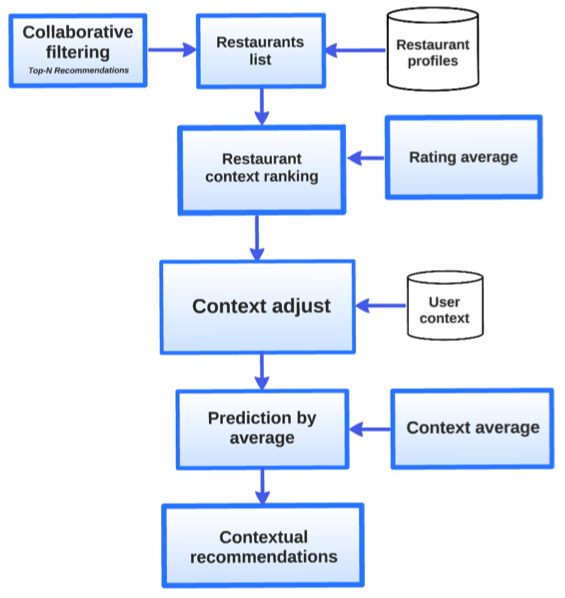
\includegraphics[width=0.50\textwidth]{img/posfil.png}
\caption{The post-filtering approach for Tijuana restaurants.}
\label{fig:postfiltering}     
\end{figure*}
%%%%%%%%%%%%
In order to validate the proposed approach,  data  about 
restaurant preferences of users in different contexts was used.
The study subjects were students  with a major in engineering and  
a graduate program and faculty of the Tijuana Institute of
Technology. A total of \textit{50 users} answered a questionnaire; the
questions were about their preferences for nearby restaurants and the
technology most often used by them. The \textit{questionnaire} consisted 
of \textit{8 questions} and also they were asked to rate any number 
of restaurants from a list of 40 restaurants.
Each of the restaurants chosen, was rated 6 times one per proposed 
context, a matrix rating with \textit{1,422 ratings} was collected. The
questions are shown in table \ref{tab:questions}. The reason for allowing
users to chose what restaurants to rate it to give them the same liberty
that they have when visiting a web or mobile application. 
>>>>>>> origin/master
\begin{table}
\small
\captionsetup{font=footnotesize}
\caption{Questionnaire applied to collect contextual dataset.}
\label{tab:questions} 
\centering
\small
\begin{tabular}{p{7cm} p{5cm} }
\hline\noalign{\smallskip}
Question & Answers \\
\noalign{\smallskip}\hline\noalign{\smallskip}
\small{1.What is your occupation?} & \small{1. Student 2.Faculty} \\ \hline  
\small{2.According to your priority, order by importance the features 
you consider when you choose to visit a restaurant.} & 
\small{1.Installation/decoration 2.Prices 3.Service 4.Dishes
5.Atmosphere 6.Location} \\ \hline  
\small{3.What devices do you use} &
\small{1.Smartphone 2.Tablet 3.Laptop 4.PC} \\ \hline   
\small{4.What Operating System do you use?} & 
\small{1.Android 2.Windows 3.iOS 4.Symbian 5.Blackberry 6.Other}
\\ \hline  
\small{5.Did you use an application to search restaurants in Tijuana?} &
\small{1.Yes 2.No 3.Which one?} \\ \hline   
\small{6.Would you like to use an application of
recommender systems of Tijuana?} & \small{1.Yes 2.No} \\ \hline  
\small{7.Please, rates your favorites restaurants(without context).} & 
\small{Restaurant list} \\ \hline
\small{8.Please, rates your favorites restaurants in contextual situations.} & 
\small{Restaurant list} \\
\noalign{\smallskip}\hline
\end{tabular}
\end{table}
<<<<<<< HEAD
In order to validate the proposed approach,  data  about 
restaurant preferences of users in different contexts was used.
The study subjects were students  with a major in engineering and  
a graduate program and faculty of the Tijuana Institute of
Technology.\\ A total of \textit{50 users} answered a questionnaire; the
questions were about their preferences for nearby restaurants and the
technology most often used by them. The \textit{questionnaire} consisted 
of \textit{eigth questions} and also they were asked to rate any number 
of restaurants from a list of 40 restaurants.
Each of the restaurants chosen, was rated six times one per proposed 
context, a matrix rating with \textit{1,422 ratings} was collected. The
questions are shown in Table  \ref{tab:questions}. \\The reason for allowing
users to chose what restaurants to rate it to give them the same liberty
that they have when visiting a web or mobile application. 
=======
The users' answers from question 1 to question 6 are represented in
the figure \ref{fig:cakeschart}. \textit{Figure \ref{fig:cakeschart}a}
represents the percentage of surveyed students and teachers;
\textit{figure \ref{fig:cakeschart}b}  the percentage of the element
that users consider the most important to visit a restaurant;
\textit{figure \ref{fig:cakeschart}c} represents the preferences of
devices when are using Internet for restaurant recommendations;
\textit{figure \ref{fig:cakeschart}d} represents the percentage of
operating system that often used, \textit{figure
\ref{fig:cakeschart}e} shows the percentage of users that use the
Internet to search restaurants in Tijuana; and \textit{figure
\ref{fig:cakeschart}f}, shows the percentage of users that would like
using a restaurant recommender system of Tijuana.
>>>>>>> origin/master
\begin{figure*}
\captionsetup{justification=centering,margin=2cm,font=footnotesize}
\centering
\setlength\fboxsep{0pt}
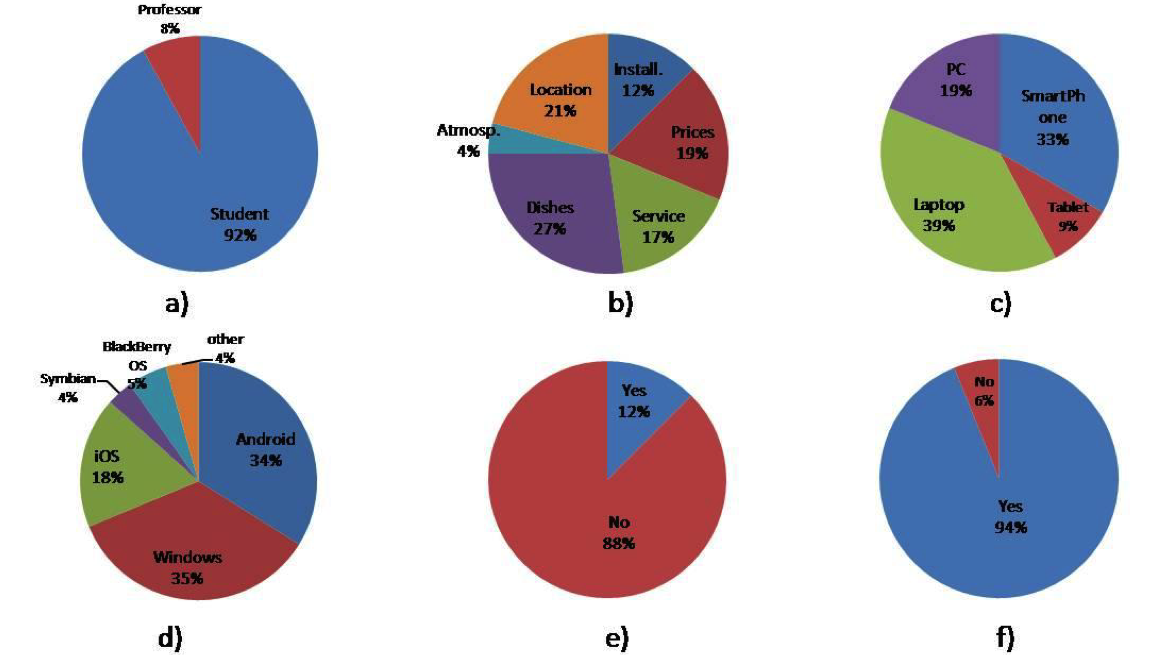
\includegraphics[width=0.8\textwidth]{img/cakes.png}
<<<<<<< HEAD
\caption{The chart cakes show the users preferences for questions from one to six.}
\label{fig:cakeschart}     
\end{figure*}
The users' answers from question one to question six are represented in
the Figure  \ref{fig:cakeschart}. Figure  \textit{\ref{fig:cakeschart}a}
represents the percentage of surveyed students and teachers;
Figure  \textit{\ref{fig:cakeschart}b}  the percentage of the element
that users consider the most important to visit a restaurant;
Figure  \textit{\ref{fig:cakeschart}c} represents the preferences of
devices when are using Internet for restaurant recommendations;
Figure  \textit{\ref{fig:cakeschart}d} represents the percentage of
operating system that often used, 
Figure  \textit{\ref{fig:cakeschart}e} shows the percentage of users 
that use the Internet to search restaurants in Tijuana; and 
Figure  \textit{\ref{fig:cakeschart}f}, shows the percentage of users 
that would like using a restaurant recommender system of Tijuana.
=======
\caption{The chart cakes show the users preferences for questions from 1 to 6.}
\label{fig:cakeschart}     
\end{figure*}
For questions 7 and 8 only the top-ten restaurants are shown,
without/with the contextual situation. In figure \ref{fig:barschart}a,
the favorite restaurant is \textbf{Daruma}(178 votes),  whereas in
figure \ref{fig:barschart}b, \textbf{Daruma} does not appear in the
top-ten. When considering the context \textit{midweek}, the favorite
restaurant was \textbf{Carl's Jr.}, which appears in both graphs; this
restaurant was also the most voted in the different contexts.
>>>>>>> origin/master
\begin{figure*}
\captionsetup{justification=centering,margin=2cm,font=footnotesize}
\centering
\setlength\fboxsep{0pt}
%\setlength\fboxrule{0.7pt}
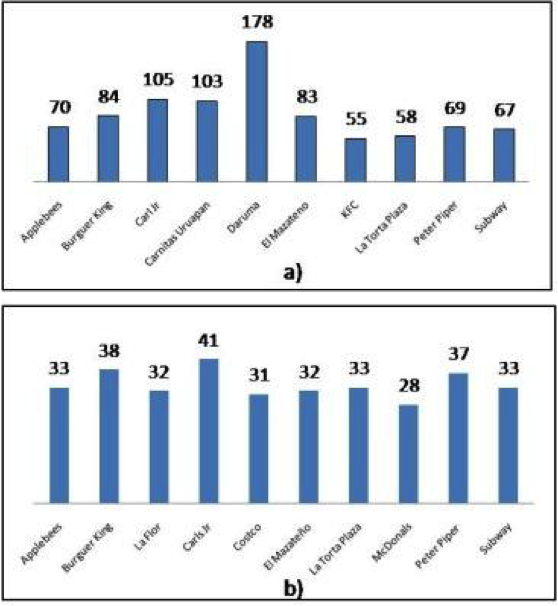
\includegraphics[width=0.55\textwidth]{img/bars.png}
<<<<<<< HEAD
\caption{The chart of users preferences for questions seven and eigth.}
\label{fig:barschart}     
\end{figure*}
\\For questions seven and eigth only the top-ten restaurants are shown,
without/with the contextual situation. In Figure  \textit{\ref{fig:barschart}a},
the favorite restaurant is \textbf{Daruma}(178 votes),  whereas in
Figure  \textit{\ref{fig:barschart}b}, \textbf{Daruma} does not appear in the
top-ten. \\When considering the context \textit{midweek}, the favorite
restaurant was \textbf{Carl's Jr.}, which appears in both graphs; this
restaurant was also the most voted in the different contexts.
Contextual recommendations of post-filtering approach depends of
context \textit{midweek} or \textit{weekend}, which is the day when
the restaurants were rated. \\Subsequently, the result of the query is
refined according to the user context; the six contexts mentioned
correspond to combinations of contextual factors shown in 
Table  \ref{tab:contextstijuana}.
=======
\caption{The chart shows the users preferences for questions 7 and 8.}
\label{fig:barschart}     
\end{figure*}
Contextual recommendations of post-filtering approach depends of
context \textit{midweek} or \textit{weekend}, which is the day when
the restaurants were rated. Subsequently, the result of the query is
refined according to the user context; the 6 contexts mentioned
correspond to combinations of contextual factors shown in table
\ref{tab:contextstijuana}.
>>>>>>> origin/master
\begin{table}
\small
\captionsetup{font=footnotesize}
\caption{Contextual factors considered in the questionnaire.}
\label{tab:contextstijuana} 
\centering
<<<<<<< HEAD
\begin{tabular}{p{2.0cm} p{10cm} }
\hline\noalign{\smallskip}
Contextual Factor & Context \\
\noalign{\smallskip}\hline\noalign{\smallskip}
\small{Day} & \small{1.Midweek (Monday, Thuesday,Wednesday and Thursday)
2.Weekend (Friday,Saturday and Sunday)}  \\ \hline 
=======
\begin{tabular}{p{2.5cm} p{7cm} }
\hline\noalign{\smallskip}
Contextual Factor & Context \\
\noalign{\smallskip}\hline\noalign{\smallskip}
\small{Day} & \small{1.Midweek(Monday, Thuesday,Wednesday and Thursday)
2.Weekend(Friday,Saturday and Sunday)}  \\ \hline 
>>>>>>> origin/master
\small{Place} & \small{1.School 2. Home 3.Work} \\ 
\noalign{\smallskip}\hline
\end{tabular}
\end{table}
<<<<<<< HEAD
Mean absolute error obtained was \textbf{0.5859}  in contextual
recommendations.  The observation for this result is that using a
small dataset the performance of the method proposed is limited, the
cold-start  problem affects the accuracy because of the data scarcity.

\section{Hotels recommendations} \label{hotels}

A second experiment using TripAdvisor's dataset was cunducted.  For
this case, the proposed method consisted of three algorithms  to
recommend:  \textit{fuzzy inference system}, \textit{collaborative
filtering} and \textit{content-based}. Each one uses the ratings
matrix to get recommendations.\\     The contextual recommender system
uses  \textit{post-filtering} approach  \cite{adomavicius2011context}
for adjust recommendations in context such as restaurants. 
The recommendation by popularity is  through the fuzzy inference system
depicted in Figure  \ref{fig:fis},  the fuzzy inference system
contains the variables that are involved in the process to recommend
in a human interaction, this process is the same that the recommender
system does. \\The output represents how matter each item into the
users community, i.e. if it is a popular item between users. \\ The
dataset used to evaluate the algorithm was TripAdvisor in two versions
downloaded  \cite{linkzeng}, this datasets was used in
\cite{zheng2014context} and  \cite{zheng2012differential} to  evaluate
the performance of context-aware recommender systems. \\The first
dataset contains 4669 contextual ratings, 1202 users and 1890 hotels;
the second dataset contains 14175 contextual ratings, 2731 users and
2269 hotels. 
\begin{figure*}
\captionsetup{justification=centering,margin=2cm,font=footnotesize}
\centering
\setlength\fboxsep{0pt}
\setlength\fboxrule{0.7pt}
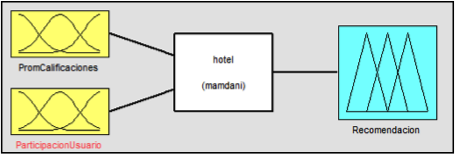
\includegraphics[width=0.75\textwidth]{img/fis.png}
\caption{Fuzzy inference system.}
\label{fig:fis}   
\end{figure*}
Data were collected of reviews online in tripadvisor.com.
There is only one context: \textit{type of trip} (family, friends,
bussines, romantic and relax).\\  The FIS has Gaussians membership
functions and are depicted in  Figure  \ref{fig:mffis}.
=======
The  mean absolute error obtained was \textbf{0.5859} 
in contextual recommendations. 
The observation for this result is that using a small
dataset the performance of the method proposed is limited, the cold-start 
problem affects the accuracy because of the data scarcity.

\section{Hotels recommendations} \label{hotels}

A second experiment using TripAdvisor's dataset was cunducted. 
For this case, the proposed method consisted of three algorithms 
to recommend:  \textit{fuzzy inference system}, \textit{collaborative 
filtering} and \textit{content-based}. Each one uses the ratings 
matrix to get recommendations.\\    
The contextual recommender system uses  \textit{post-filtering}
approach\cite{adomavicius2011context} for adjust recommendations in
context such as restaurants. The recommendation by popularity is 
through the fuzzy inference system depicted in figure \ref{fig:fis}, 
the fuzzy inference
system contains the variables that are involved in the process to
recommend in a human interaction, this process is the same that the
recommender system does. \\The output represents how matter each item
into the users community, i.e. if it is a popular item between users. \\
The dataset used to evaluate the algorithm was TripAdvisor in two
versions downloaded\cite{linkzeng}, this datasets was used in
\cite{zheng2014context} and \cite{zheng2012differential} to  evaluate the
performance of context-aware recommender systems. \\The first
dataset contains 4669 contextual ratings, 1202 users and 1890 hotels;
the second dataset contains 14175 contextual ratings, 2731 users and
2269 hotels. Data were collected of reviews online in tripadvisor.com.
There is only one context: \textit{type of trip} (family, friends, bussines,
romantic and relax).\\ 
The FIS has Gaussians membership functions and are depicted in figure
\ref{fig:mffis}.
>>>>>>> origin/master
\begin{figure}[ht!]
   \captionsetup{font=footnotesize}
   \centering
   %%----primera subfigura----
   \subfloat[]{
        \label{fig:1a}
        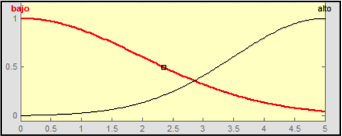
\includegraphics[width=0.42\textwidth]{img/ratingaverage.png}}
   \hspace{0.1\linewidth}
   %%----segunda subfigura----
   \subfloat[]{
        \label{fig:1b} 
        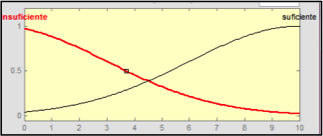
\includegraphics[width=0.42\textwidth]{img/userparticipation.png}}\\[20pt]
   %%----tercera subfigura----
    \subfloat[]{
        \label{fig:1c} 
        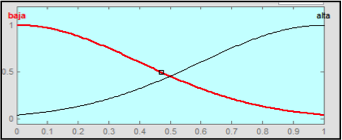
\includegraphics[width=0.42\textwidth]{img/recommendation.png}}
   \caption{Gaussian Membership functions in the input are: a) RatingAverage, 
   b) UserParticipation, and an output: c) Recommendation.}
   \label{fig:mffis} 
\end{figure}
The fuzzy inference system uses fuzzy rules to infer the inputs and 
output(a crisp value) that represents the weight of the recommendation. 
The rules are following: 
\begin{enumerate}
\item \textit{If \textbf{RatingAverage} is low and 
\textbf{UserParticipation} is insufficient then \textbf{recommendation} is low.}
\item \textit{If \textbf{RatingAverage} is low and 
\textbf{UserParticipation} is sufficient then \textbf{recommendation} is high.}
\item \textit{If \textbf{RatingAverage} is high and 
\textbf{UserParticipation} is insufficient then \textbf{recommendation} is low.}
\item \textit{If \textbf{RatingAverage} is high and 
\textbf{UserParticipation} is sufficient then \textbf{recommendation} is high.}
\end{enumerate}
<<<<<<< HEAD
=======
\begin{figure*}
\captionsetup{justification=centering,margin=2cm,font=footnotesize}
\centering
\setlength\fboxsep{0pt}
\setlength\fboxrule{0.7pt}
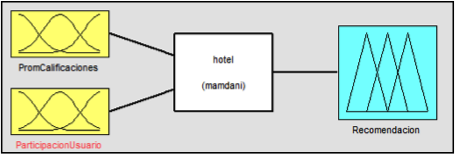
\includegraphics[width=0.75\textwidth]{img/fis.png}
\caption{Fuzzy inference system.}
\label{fig:fis}   
\end{figure*}
>>>>>>> origin/master
Content-based uses cosine similarity to compare the binary
vectors representing the profile of each item, thereby obtaining a
numerical value that determines similarity, based on a threshold. \\   
In other words, it makes a comparison of profiles of each item to
determine the most similar to items the user has rated with highest
score, context-aware recommender system proposed has a scale 
<<<<<<< HEAD
from 1 to 5. \\
Next, the outputs of every recommender technique is represented by a
list of recommended items. Subsequently applies the context filter and
context-aware recommender system gets the final contextual
recommendations.\\  Context-aware recommender system identifies
contextual data of the user profile such as in Table  \ref{tab:2}, and
compares recommended items to filter those items that are adjusted to
the user context.  
=======
from 1 to 5. 
>>>>>>> origin/master
\begin{table}[htb]
\small
\centering
\captionsetup{font=footnotesize}
\caption{Example of contextual ratings in the user profile.}
\label{tab:2}
\small
\begin{tabular}{lll}
\hline
\multicolumn{3}{c}{\textbf{User profile}} \\ \hline
Item & Rating & Context \\ \hline
La Casa del Mole & 5.0 & Midweek \\ 
Daruma           & 4.0 & Weekend \\ 
Daruma           & 5.0 & Midweek \\ 
Carl's Jr.       & 3.0 & Weekend \\ \hline
\end{tabular}
\end{table}
<<<<<<< HEAD
The context filtering is the last step before to
get the recommended items. \\The schema of architecture for context-
aware recommender system is depicted in Figure  \ref{fig:architecture}.
=======
Next, the outputs of every recommender technique is represented by a
list of recommended items. Subsequently applies the context filter and
context-aware recommender system gets the final contextual
recommendations. Context-aware recommender system identifies
contextual data of the user profile (see table \ref{tab:2}), and
compares recommended items to filter those items that are adjusted to
the user context.  The context filtering is the last step before to
get the recommended items. The schema of architecture for context-
aware recommender system is depicted in figure \ref{fig:architecture}.
>>>>>>> origin/master
\begin{figure*}
\captionsetup{font=footnotesize}
%\captionsetup{justification=centering,margin=2cm}
\centering
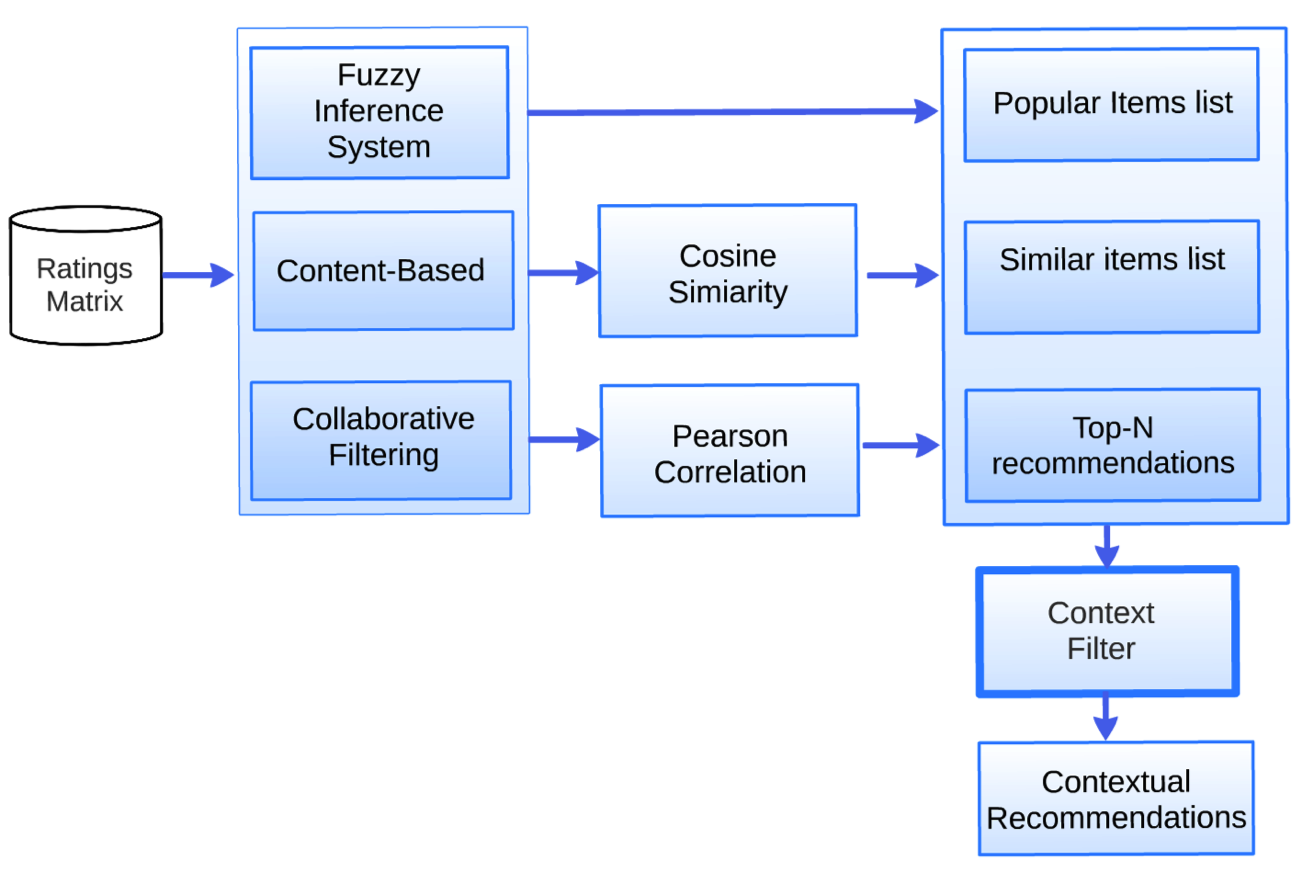
\includegraphics[width=0.80\textwidth]{img/archit-ta.png}
\caption{Recommender system methodology.}
\label{fig:architecture}   
\end{figure*}
<<<<<<< HEAD
Two tests were performed using TripAdvisor dataset, 
Table  \ref{tab:3} describes the data sets and the scarcity percentage of the
specified data. \\ Scarcity of 99\% mean that there are problems to
recommend items because the information is not enought to get 
good recommendations.
=======
Two tests were performed using TripAdvisor dataset, table
\ref{tab:3} describes the data sets and the scarcity percentage of the
specified data. Scarcity of 99\% mean that there are problems to
recommend items because the information is not enought to get 
good recommendations.\\  By other side, in table \ref{tab:4} the comparison
shows that the algorithm has a acceptable performance, i.e., the error
falls into the range of results obtained with others algorithms. Then,
contextual recommendations were evaluated with the Root Mean Square
Error in order to compare the results with context relaxation
algorithm\cite{zheng2012differential} that is evaluated with the same
dataset.
>>>>>>> origin/master
\begin{table}
\centering
\small
\captionsetup{font=footnotesize}
\caption{Datasets description.}
\label{tab:3}      
\begin{tabular}{lllll}
\hline\noalign{\smallskip}
Dataset & Users & Items & Ratings & Scarcity (percent) \\
\noalign{\smallskip}\hline\noalign{\smallskip}
TripAdvisor v1 & 1202 & 1890 & 4669 & 99.79 \\
TripAdvisor v2 & 2731 & 2269 & 14175 & 99.77 \\
\noalign{\smallskip}\hline
\end{tabular}
\end{table}
<<<<<<< HEAD
By other side, in Table  \ref{tab:4} the comparison
shows that the algorithm has a acceptable performance, i.e., the error
falls into the range of results obtained with others algorithms. 
=======
>>>>>>> origin/master
\begin{table}
\centering
\small
\captionsetup{font=footnotesize}
<<<<<<< HEAD
\caption{Comparison of root mean square error.}
=======
\caption{Comparison of RMSE.}
>>>>>>> origin/master
\label{tab:4}  
\small   
\begin{tabular}{lll}
\hline\noalign{\smallskip}
<<<<<<< HEAD
Dataset & Algorithm & Error \\
\noalign{\smallskip}\hline\noalign{\smallskip}
TripAdvisor v2 & collaborative filtering + Post-filtering  & 0.504  \\
                        & collaborative filtering                           & 0.994  \\
                        & Pre-filtering + Relaxation                     & 0.985  \\
\noalign{\smallskip}\hline
\end{tabular}
\end{table}
Then, contextual recommendations were evaluated with the 
root mean square error in order to compare the results with context 
relaxation algorithm  \cite{zheng2012differential} that is evaluated 
with the same dataset.\\ 
The cosine similarity plays an important role in content-based because
if similarity value among items is high, the recommendations will
improve the degree of user satisfaction. This is observed when
calculating the similarity average in each dataset as shown in 
Table  \ref{tab:5}.\\ 
Fuzzy inference system can provides a list of popular items for each dataset,
recommendations through averages obtained, and recommendations are
conditioned to show it when the collaborative filtering and content-based 
are not delivering recommendations because of data scarcity.
However, the majority of popular items of dataset were rated in contexts: 
\textit{romantic, family and bussines}, that means that the dataset has
biases that affects the results.
=======
Dataset & Algorithm & RMSE \\
\noalign{\smallskip}\hline\noalign{\smallskip}
TripAdvisor v2 & FC + Post-filtering  & 0.504  \\
               & FC          & 0.994  \\
               & Pre-filtering + Relaxation & 0.985  \\
\noalign{\smallskip}\hline
\end{tabular}
\end{table}
The cosine similarity plays an important role in content-based because
if similarity value among items is high, the recommendations will
improve the degree of user satisfaction. \\ This is observed when
calculating the similarity average in each dataset as shown in table
\ref{tab:5}.
>>>>>>> origin/master
\begin{table}
\centering
\small
\captionsetup{font=footnotesize}
\caption{Level of similarity among items in datasets. }
\label{tab:5}      
\begin{tabular}{lll}
\hline\noalign{\smallskip}
Dataset  & Similarity  & Avg.votes per user. \\
\noalign{\smallskip}\hline\noalign{\smallskip}
TripAdvisor v1 & 0.448  & 5  \\
TripAdvisor v2 & 0.508  & 8  \\
\noalign{\smallskip}\hline
\end{tabular}
\end{table}
<<<<<<< HEAD

\section{Context-aware recommender system prototype} 

This section presents a context-aware recommender system prototype.
The backend have been explained in chapter  \ref{method},  in sections
 \ref{restaurants} and  \ref{hotels} talk about experiments realized
using the recommendation techniques proposed. \\ To develop the prototype
was used python language, technologies as Django Framework 1.7,
JavaScript, JQuery, Ajax, HTML5, Bootstrap 3.0  and PotsgreSQL for database.\\ 
Some dependencies and libraries were used also, it can review links of
downloads in appendix  \ref{appendixa}.
=======
Fuzzy inference system can provides a list of popular items for each dataset,
recommendations through averages obtained, and recommendations are
conditioned to show it when the collaborative filtering and content-
based are not delivering recommendations because of data scarcity.\\ 
However, the majority of popular items of dataset were rated in contexts: 
\textit{romantic, family and bussines}, that means that the dataset has
biases that affects the results.


\section{Context-aware recommender system prototype} 
This section presents a context-aware recommender system prototype.
The backend have been explained in chapter \ref{method},  in sections
\ref{restaurants} and \ref{hotels} talk about experiments realized
using the recommendation techniques proposed. \\ To develop the prototype
was used python language, technologies as Django Framework 1.7,
JavaScript, JQuery, Ajax, HTML5, Bootstrap 3.0  and PotsgreSQL for database.
Some dependencies and libraries were used also, it can review links of
downloads in appendix \ref{appendixc}.
>>>>>>> origin/master

\subsection{User Interfaces}

The system starts in a landing page, the user should do \textit{Sign in} or
<<<<<<< HEAD
\textit{Sign up} to create a new user to enter the home page. \\ 
Landing page contains the \textit{Best restaurants} rated and 
\textit{Featured top list restaurants}
proposed by users, such as shows it the Figure  \ref{fig:landing}, 
the restaurants are updated while users add ratings, 
if the tendency is changed, the section displays the change 
in the tendency. \\ The aim is to provide
=======
\textit{Sign up} to create a new user to enter the home page. 
Landing page contains the \textit{Best restaurants} rated and 
\textit{Featured top list restaurants}
proposed by users, such as shows it the figure \ref{fig:landing}, 
the restaurants are updated while users add ratings, 
if the tendency is changed, the section displays the change 
in the tendency. The aim is to provide
>>>>>>> origin/master
information for old and new users,the prototype tries to keep updated
the current preferences of users constantly.
\begin{figure*}
\captionsetup{font=footnotesize}
\centering
<<<<<<< HEAD
\fbox{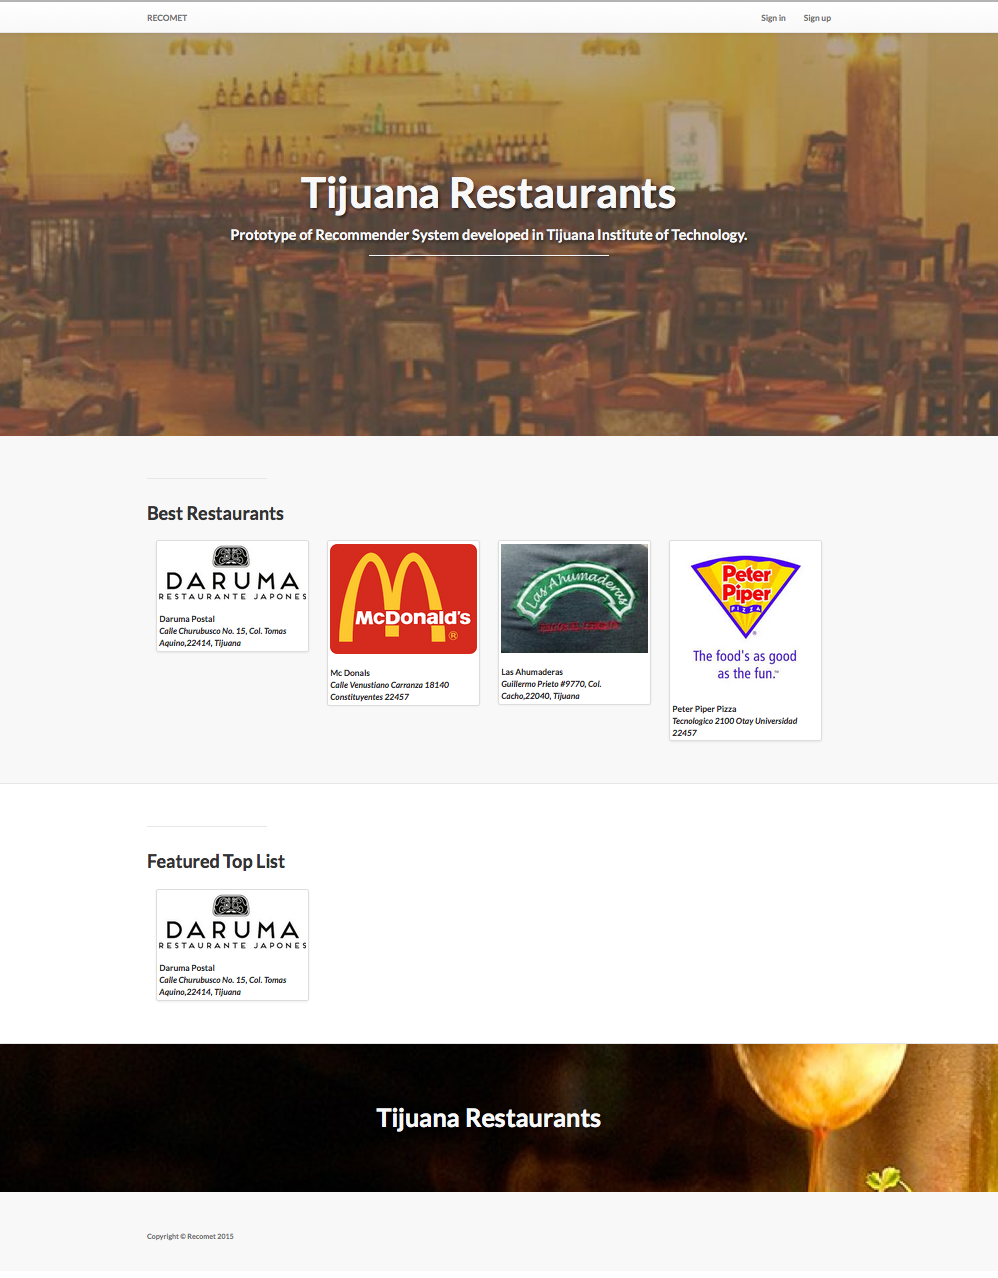
\includegraphics[width=0.60\textwidth]{img/landingpage.png}}
\caption{Landing page interface.}
\label{fig:landing}   
\end{figure*}

\subsubsection{Home Page interface}

\begin{figure*}
\captionsetup{font=footnotesize}
\centering
\fbox{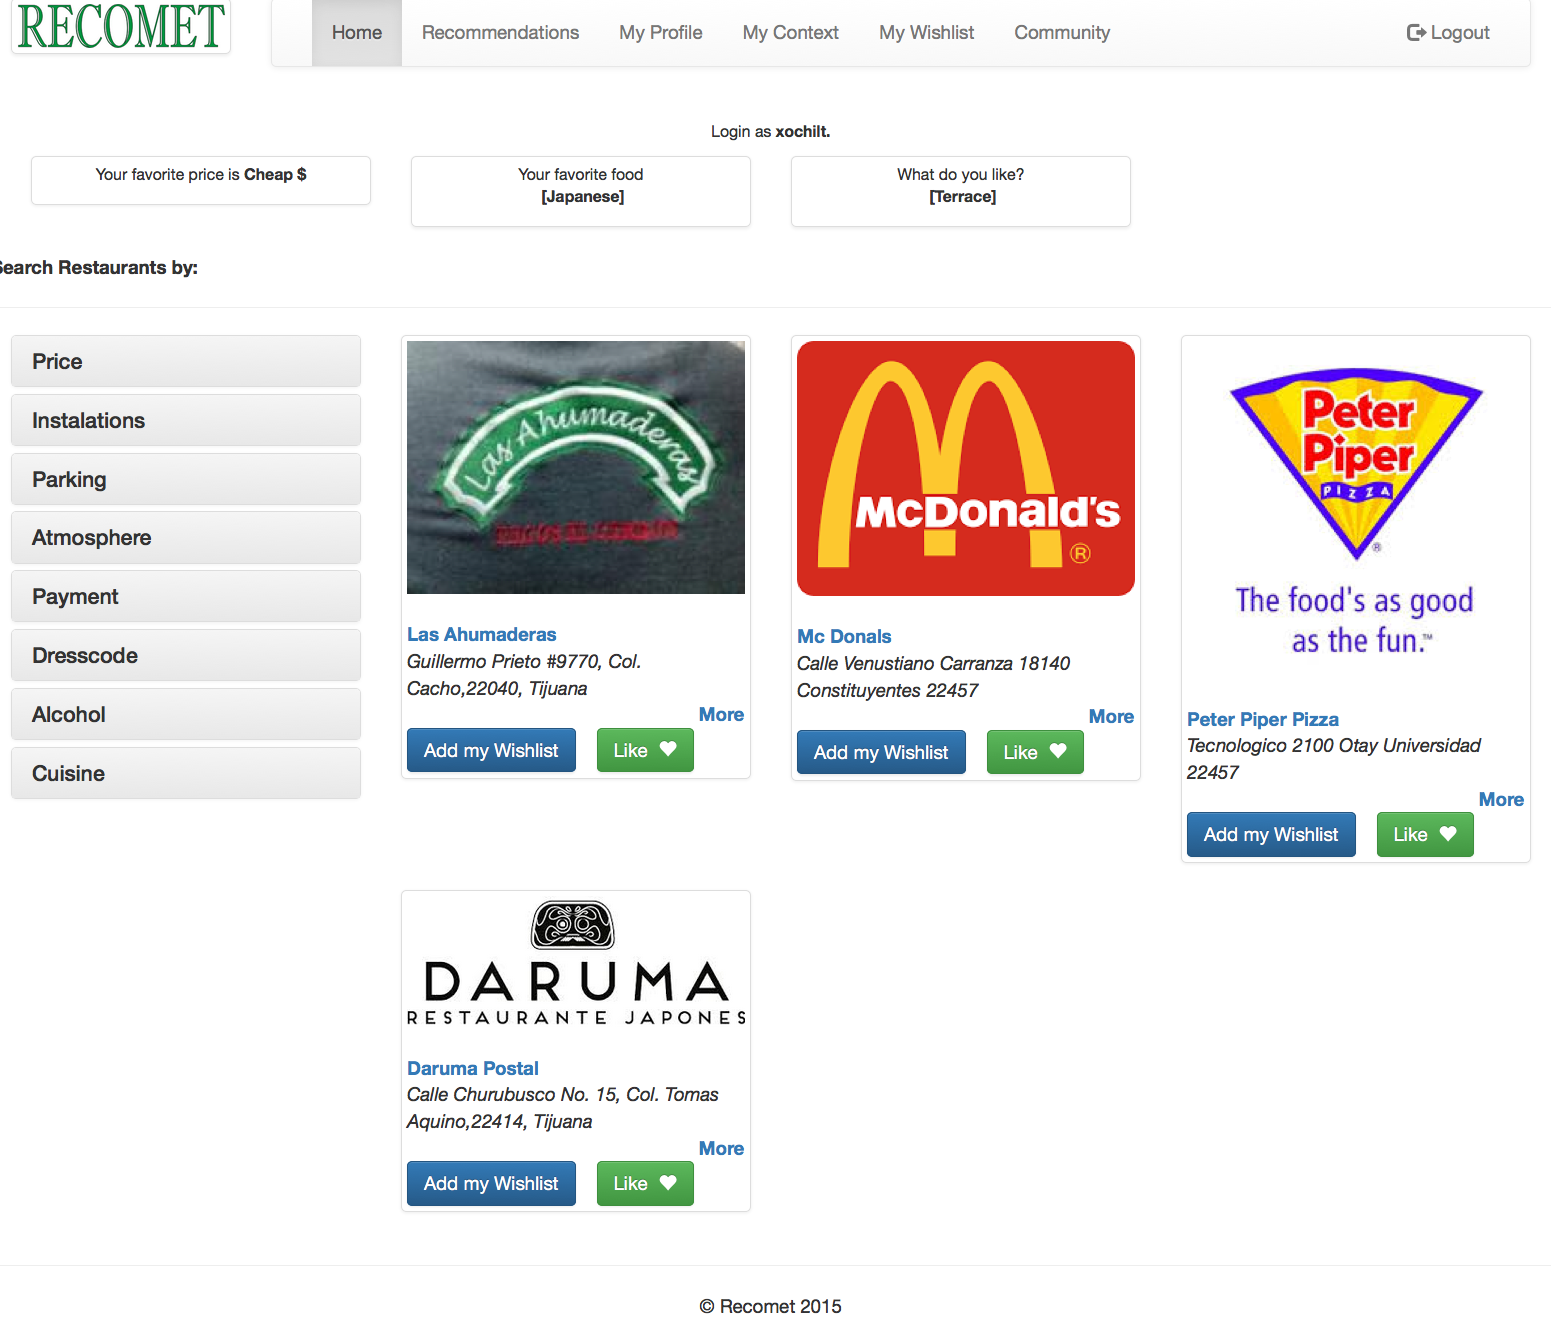
\includegraphics[width=0.60\textwidth]{img/homepage.png}}
\caption{Home page interface.}
\label{fig:home-page}   
\end{figure*}
\textit{Home Page} (Figure  \ref{fig:home-page}), shows the main
menu, tags for user preferences, all filters to start the search of
restaurants and the most popular restaurants in the community. \\ 
Users can start exploring filters to find restaurants under their own
criteria, each restaurant has a profile with complete information
about the characteristics and opinions of other users. \\ When users
click the restaurant picture the system redirects to the profile, for
instance Figure  \ref{fig:rest-profile2}  shows the profile of Daruma
restaurant, the Figure  shows the general information of the
restaurant, reviews or personal opinions of users that visited the
restaurant, details about ratings, the chart of ratings and the user
location using Google maps services. It is also added the button to
\textit{add wishlist}, this element will be explained in a posterior
section.
\begin{figure*}
\captionsetup{font=footnotesize}
\centering
\fbox{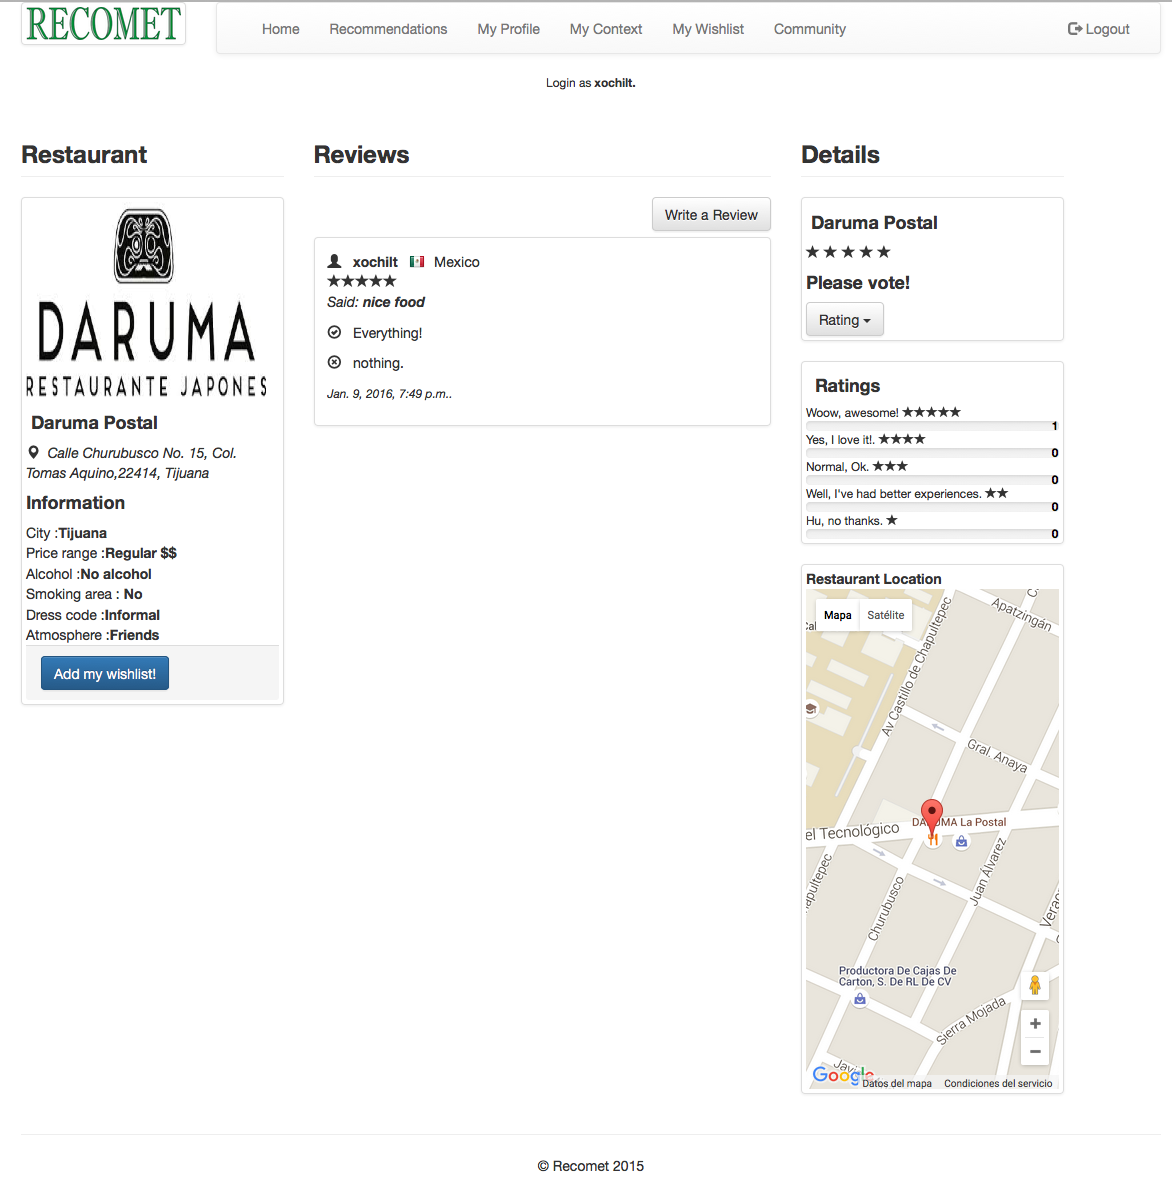
\includegraphics[width=0.60\textwidth]{img/rest-profile.png}}
\caption{Restaurant profile interface.}
\label{fig:rest-profile2}   
\end{figure*}

\subsubsection{My Recommendations interface}

\begin{figure*}
\captionsetup{font=footnotesize}
\centering
\fbox{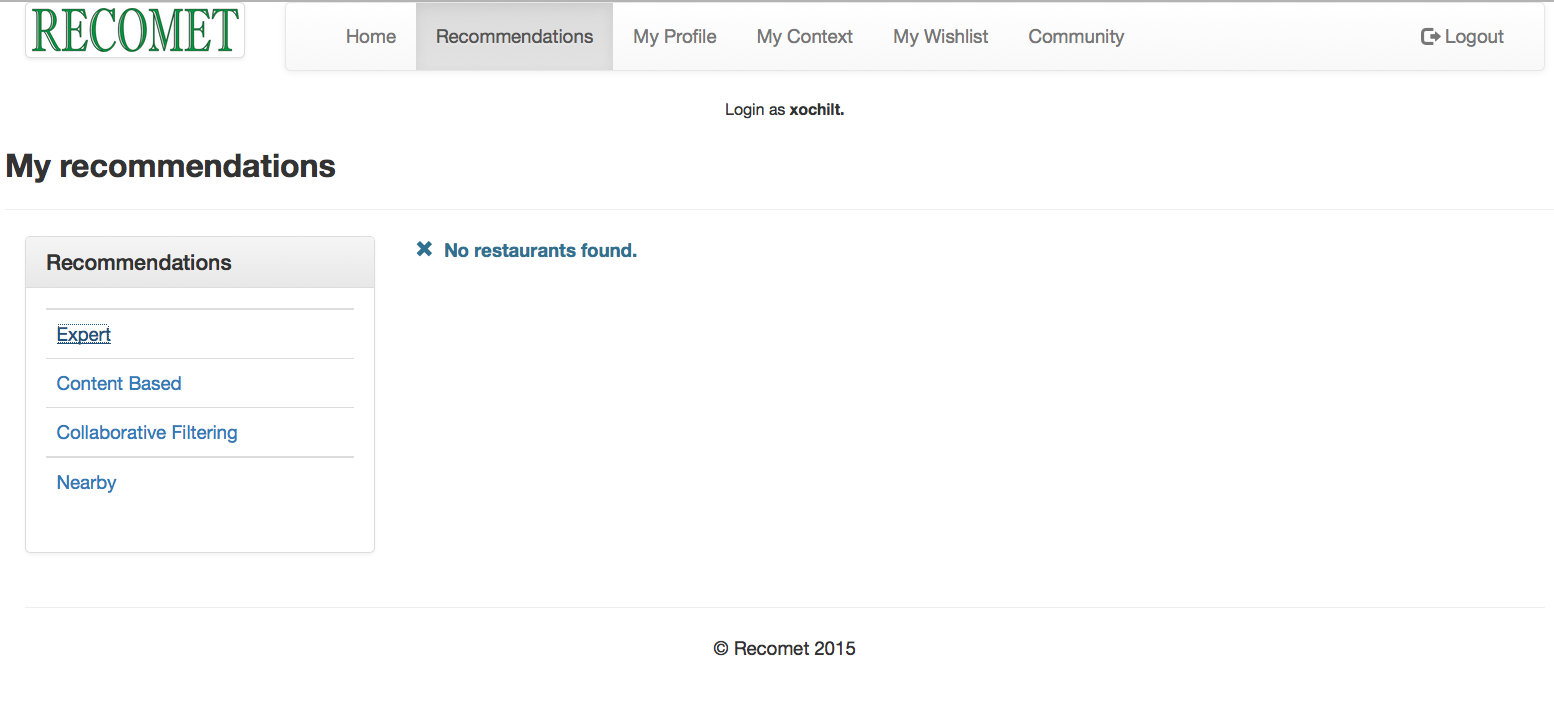
\includegraphics[width=0.60\textwidth]{img/expert-recs.png}}
=======
\fbox{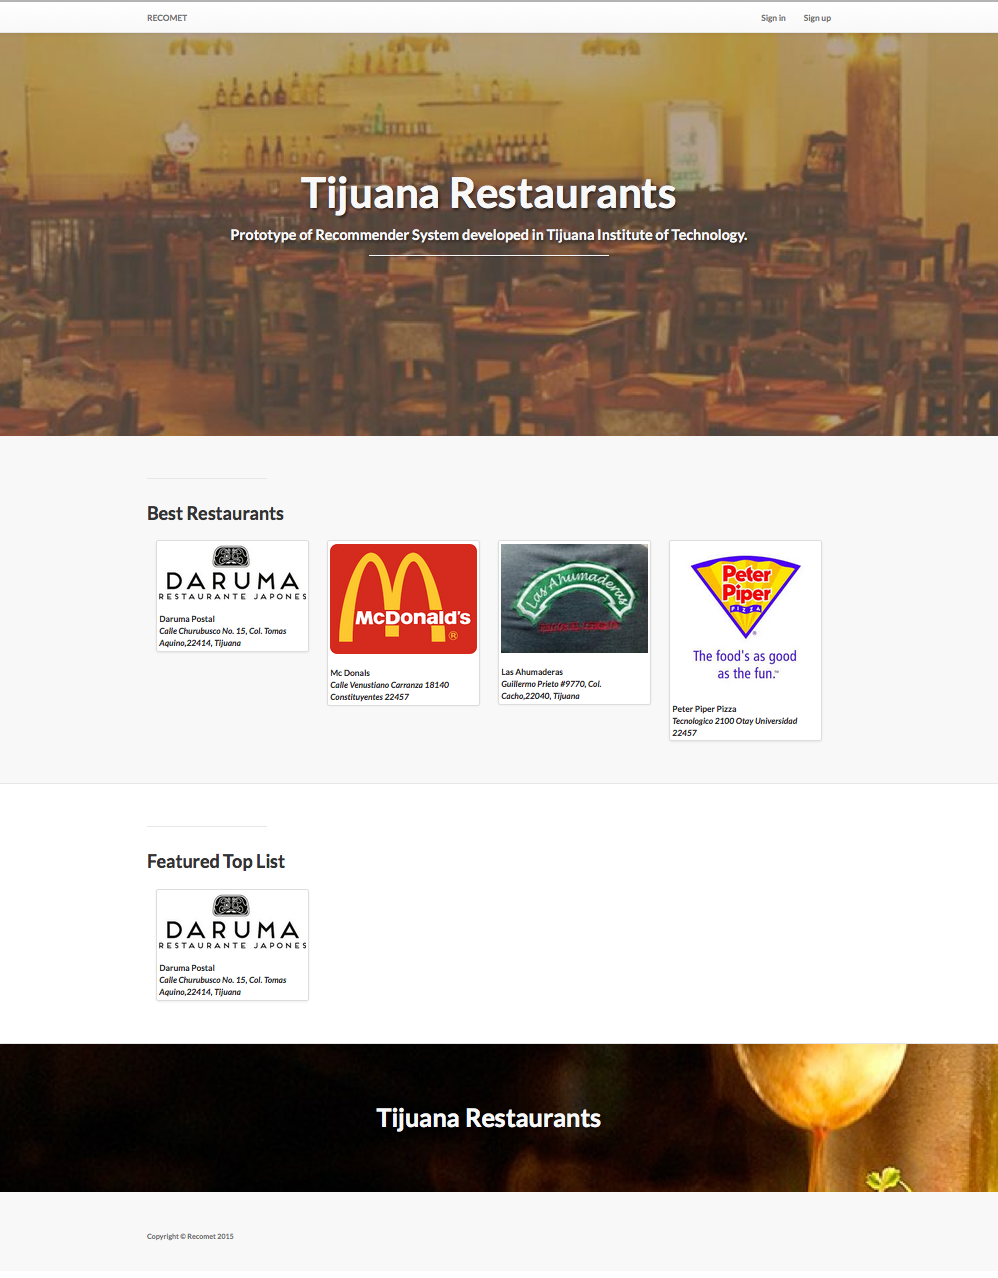
\includegraphics[width=0.70\textwidth]{img/landingpage.png}}
\caption{Landing page interface.}
\label{fig:landing}   
\end{figure*}
%%%%%%%%%%
\subsubsection{Home Page interface}
%%%%%%%%%%
\textit{Home Page} (figure \ref{fig:home-page}), shows the main 
menu, tags for user preferences,
all filters to start the search of restaurants and the most popular
restaurants in the community. Users can start exploring filters
to find restaurants under their own criteria, each restaurant has a
profile with complete information about the characteristics and
opinions of other users. When users click the restaurant picture the
system redirects to the profile, for instance figure \ref{fig:rest-profile2}  
shows the profile of Daruma restaurant, in this figure is showed the general
information of the restaurant, reviews or personal opinions of users
that visited the restaurant, details about ratings, the chart of
ratings and the user location using Google maps services. It is also
added the button to \textit{add wishlist}, this element will be explained in a
posterior section.
\begin{figure*}
\captionsetup{font=footnotesize}
\centering
\fbox{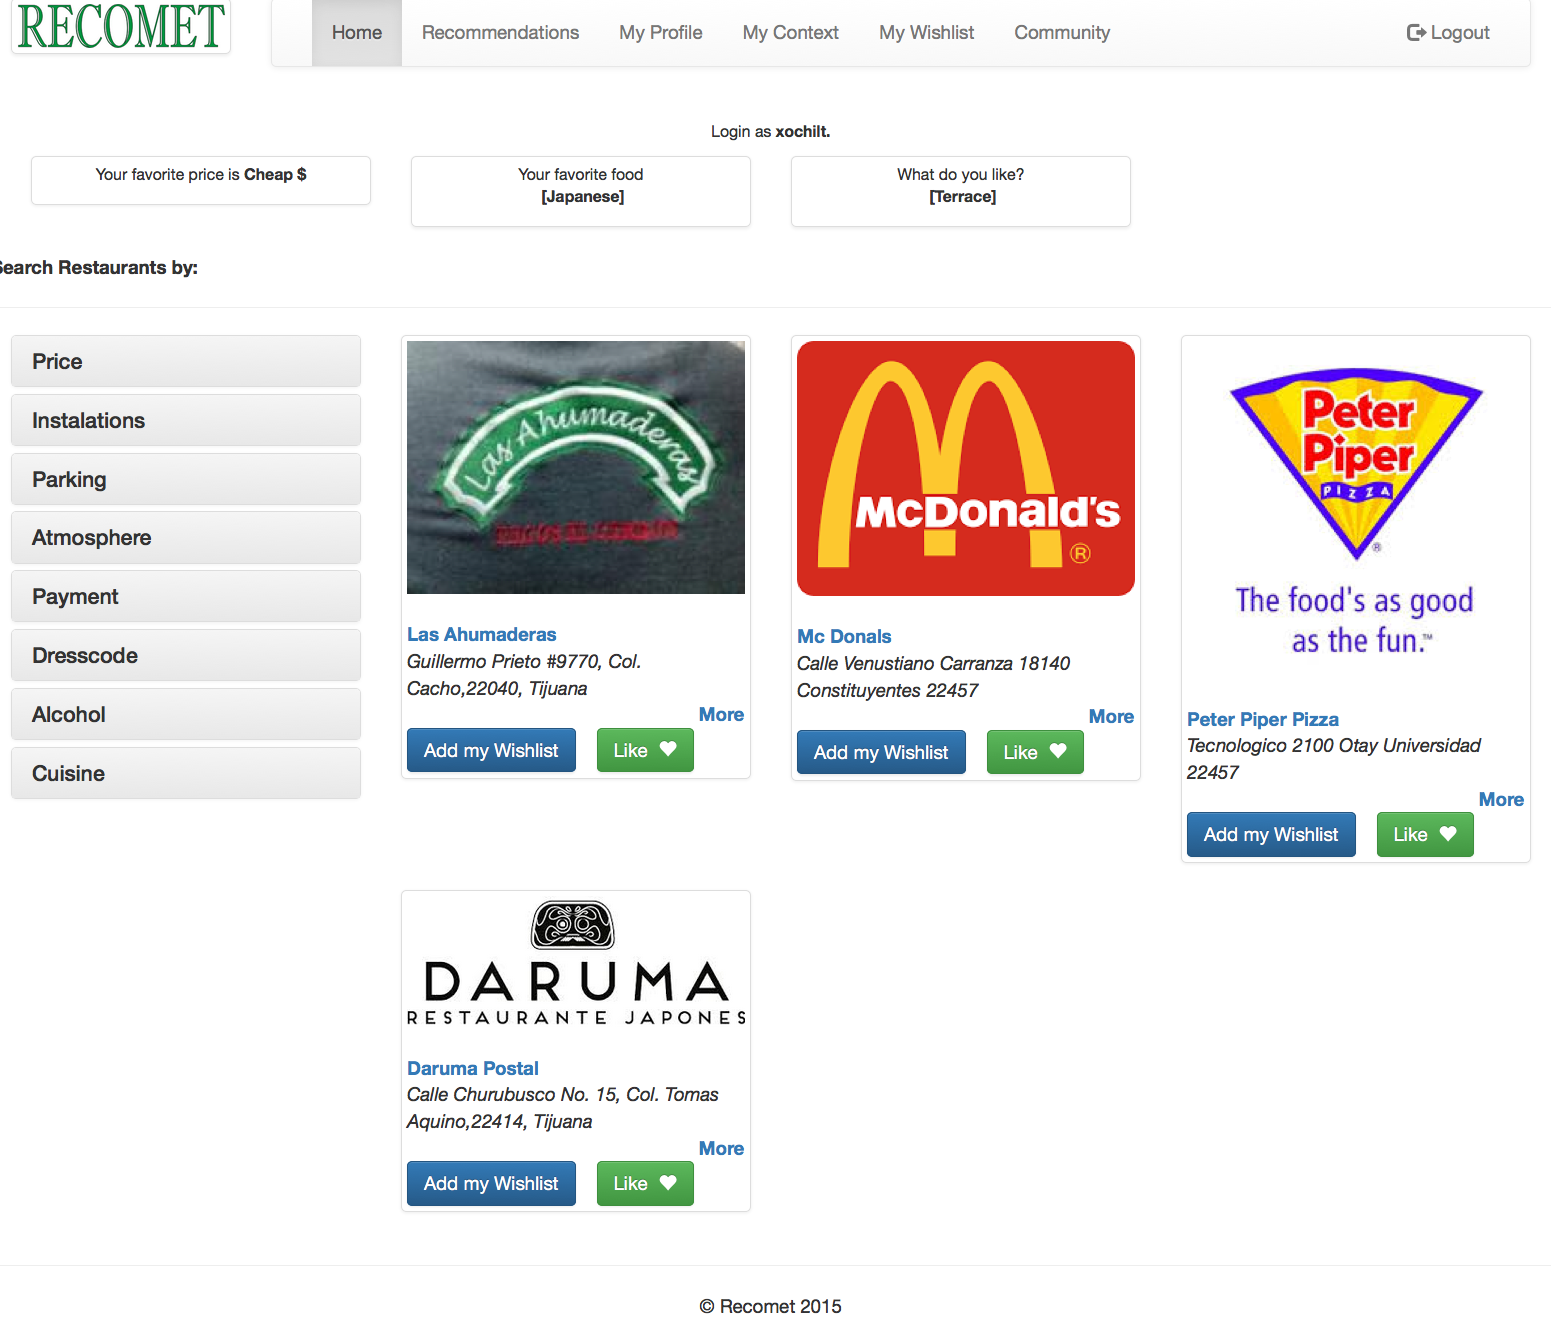
\includegraphics[width=0.70\textwidth]{img/homepage.png}}
\caption{Home page interface.}
\label{fig:home-page}   
\end{figure*}
%%%%%%%%%%%%%%%%%%%
\begin{figure*}
\captionsetup{font=footnotesize}
\centering
\fbox{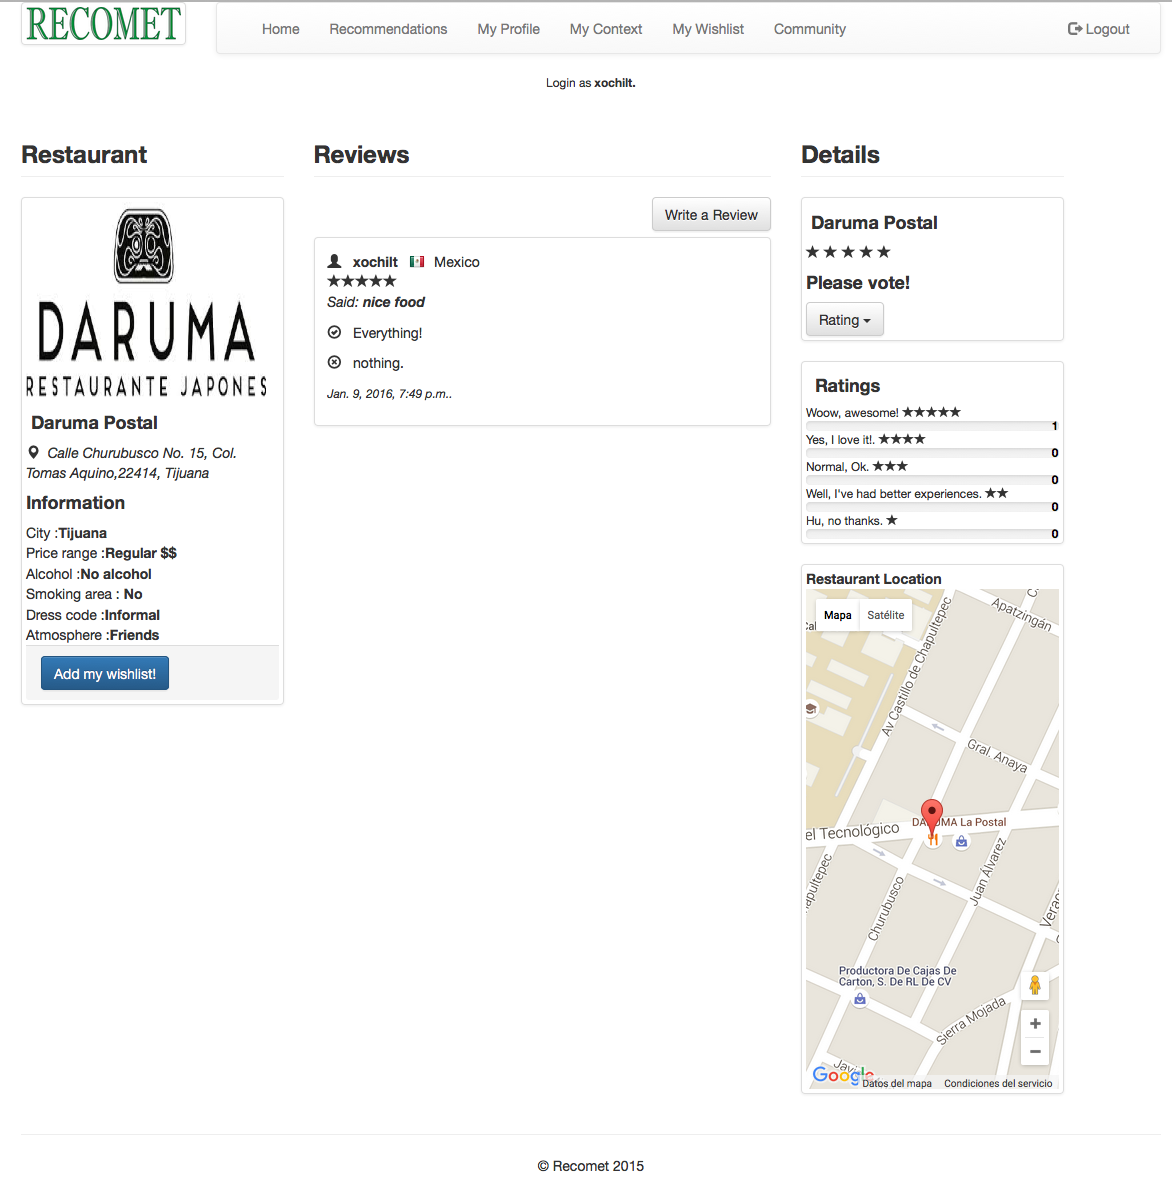
\includegraphics[width=0.70\textwidth]{img/rest-profile.png}}
\caption{Restaurant profile interface.}
\label{fig:rest-profile2}   
\end{figure*}
%%%%%%%%%%%%
\subsubsection{My Recommendations interface}
%%%%%%%%%%%%%
\begin{figure*}
\captionsetup{font=footnotesize}
\centering
\fbox{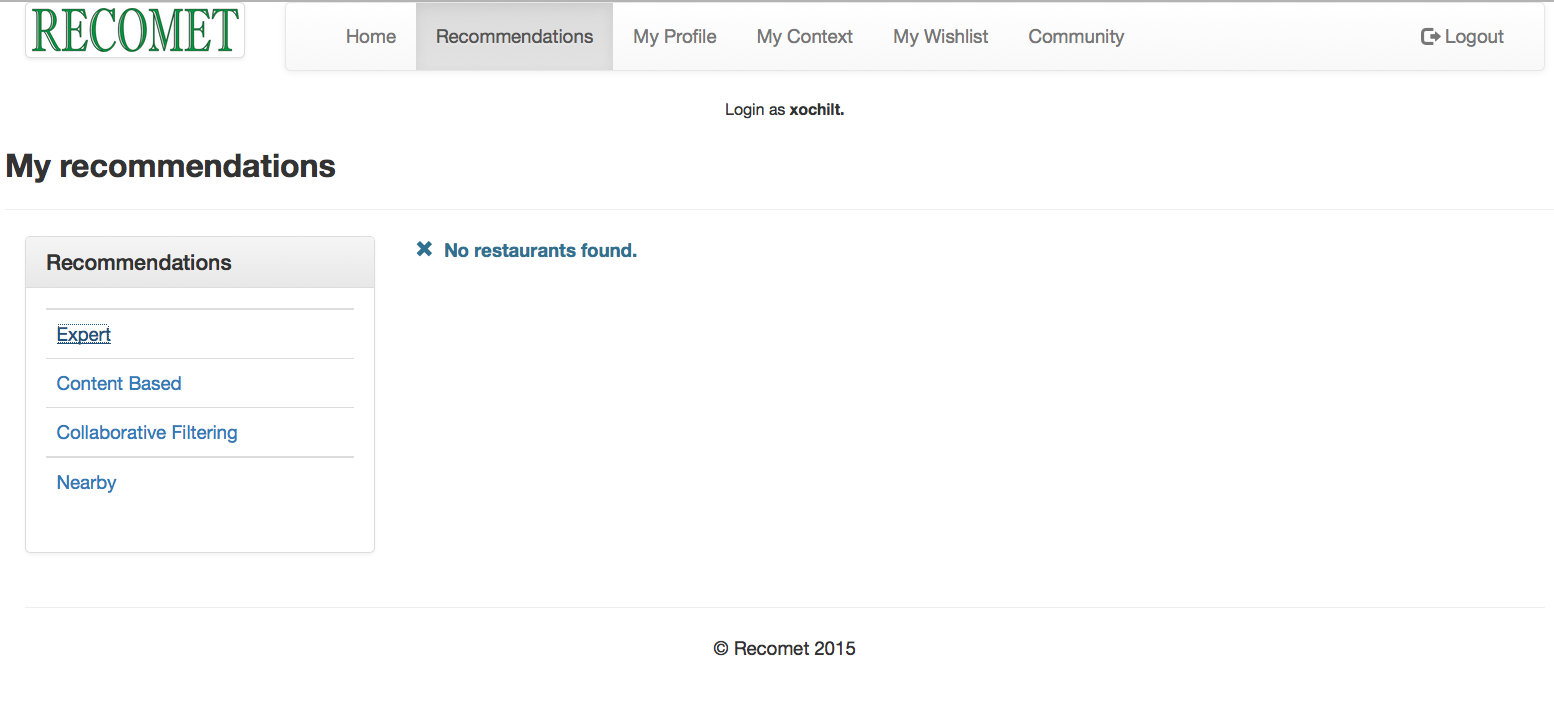
\includegraphics[width=0.70\textwidth]{img/expert-recs.png}}
>>>>>>> origin/master
\caption{Expert recommendations interface.}
\label{fig:expert-recs}   
\end{figure*}
In recommendations interface users have the options to get  
<<<<<<< HEAD
recommendations such as was described in chapter  \ref{method}, four 
recommendation techniques works to suggest restuarants for 
users. Here, users can choose the prefered option to get 
information in the screen.\\ 
For instance, Figure  \ref{fig:expert-recs} shows that the expert can 
not to recommend whether users don’t have participations, because of expert's
recommendation is based in fuzzy rules that involves the popularity of
items (input variable), if the information is sparse the prototype can
not get results and only shows an alert message. On the contrary case,
it shows a list of popular restaurants.
\begin{figure*}
\captionsetup{font=footnotesize}
\centering
\fbox{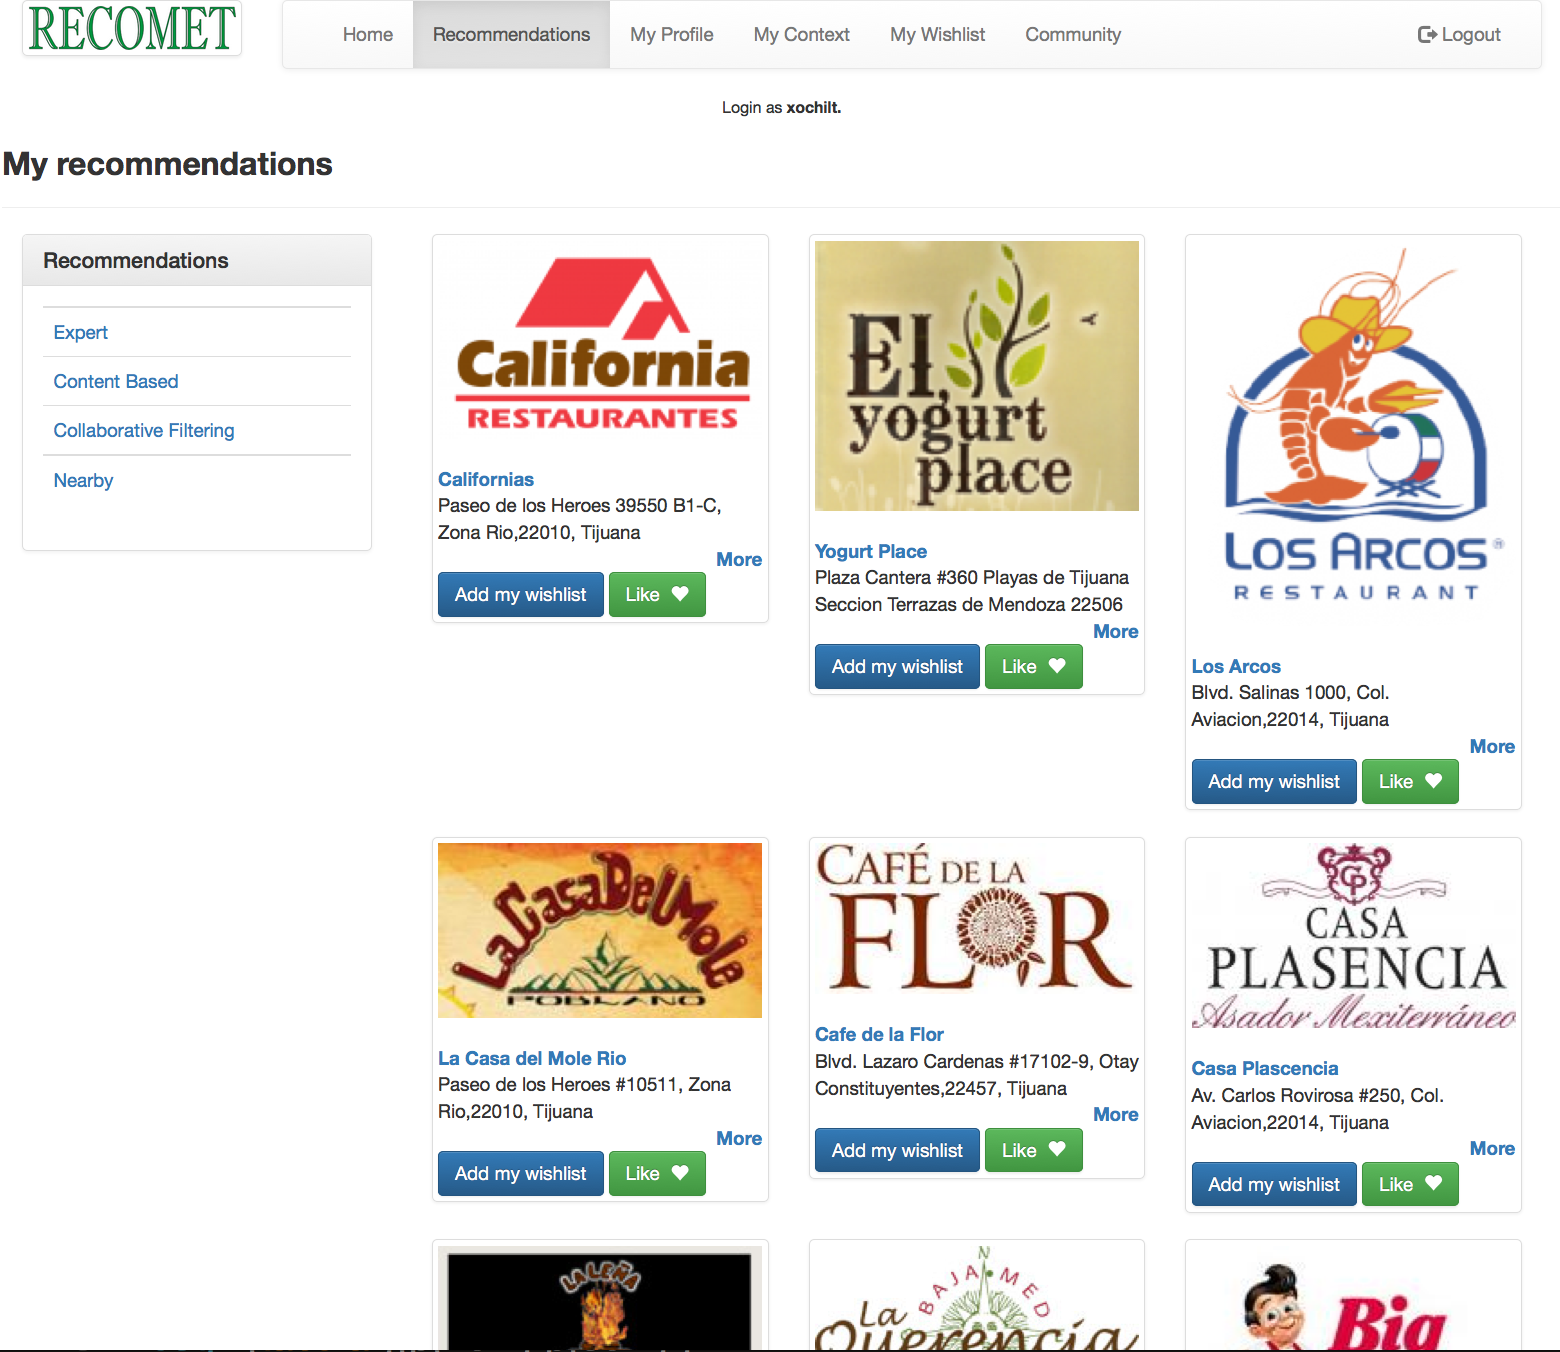
\includegraphics[width=0.60\textwidth]{img/base-content.png}}
\caption{Content-based recommendations interface.}
\label{fig:base-content}   
\end{figure*}
\\ \textit{Content-based recommendation} finds the similar restaurants to the
favorites of the user. In fact, makes a comparison of all restaurants
and gets the more similars to display in the screen. \\
Figure  \ref{fig:base-content}  
=======
recommendations such as was described in chapter \ref{method}, four 
recommendation techniques works to suggest restuarants for 
users. Here, users can choose the prefered option to get 
information in the screen.\\ 

For instance, figure \ref{fig:expert-recs} shows that the expert can 
not to recommend
whether users don’t have participations, because of expert's
recommendation is based in fuzzy rules that involves the popularity of
items (input variable), if the information is sparse the prototype can
not get results and only shows an alert message. On the contrary case,
it shows a list of popular restaurants.\\ 
%%%%%%%%%
\begin{figure*}
\captionsetup{font=footnotesize}
\centering
\fbox{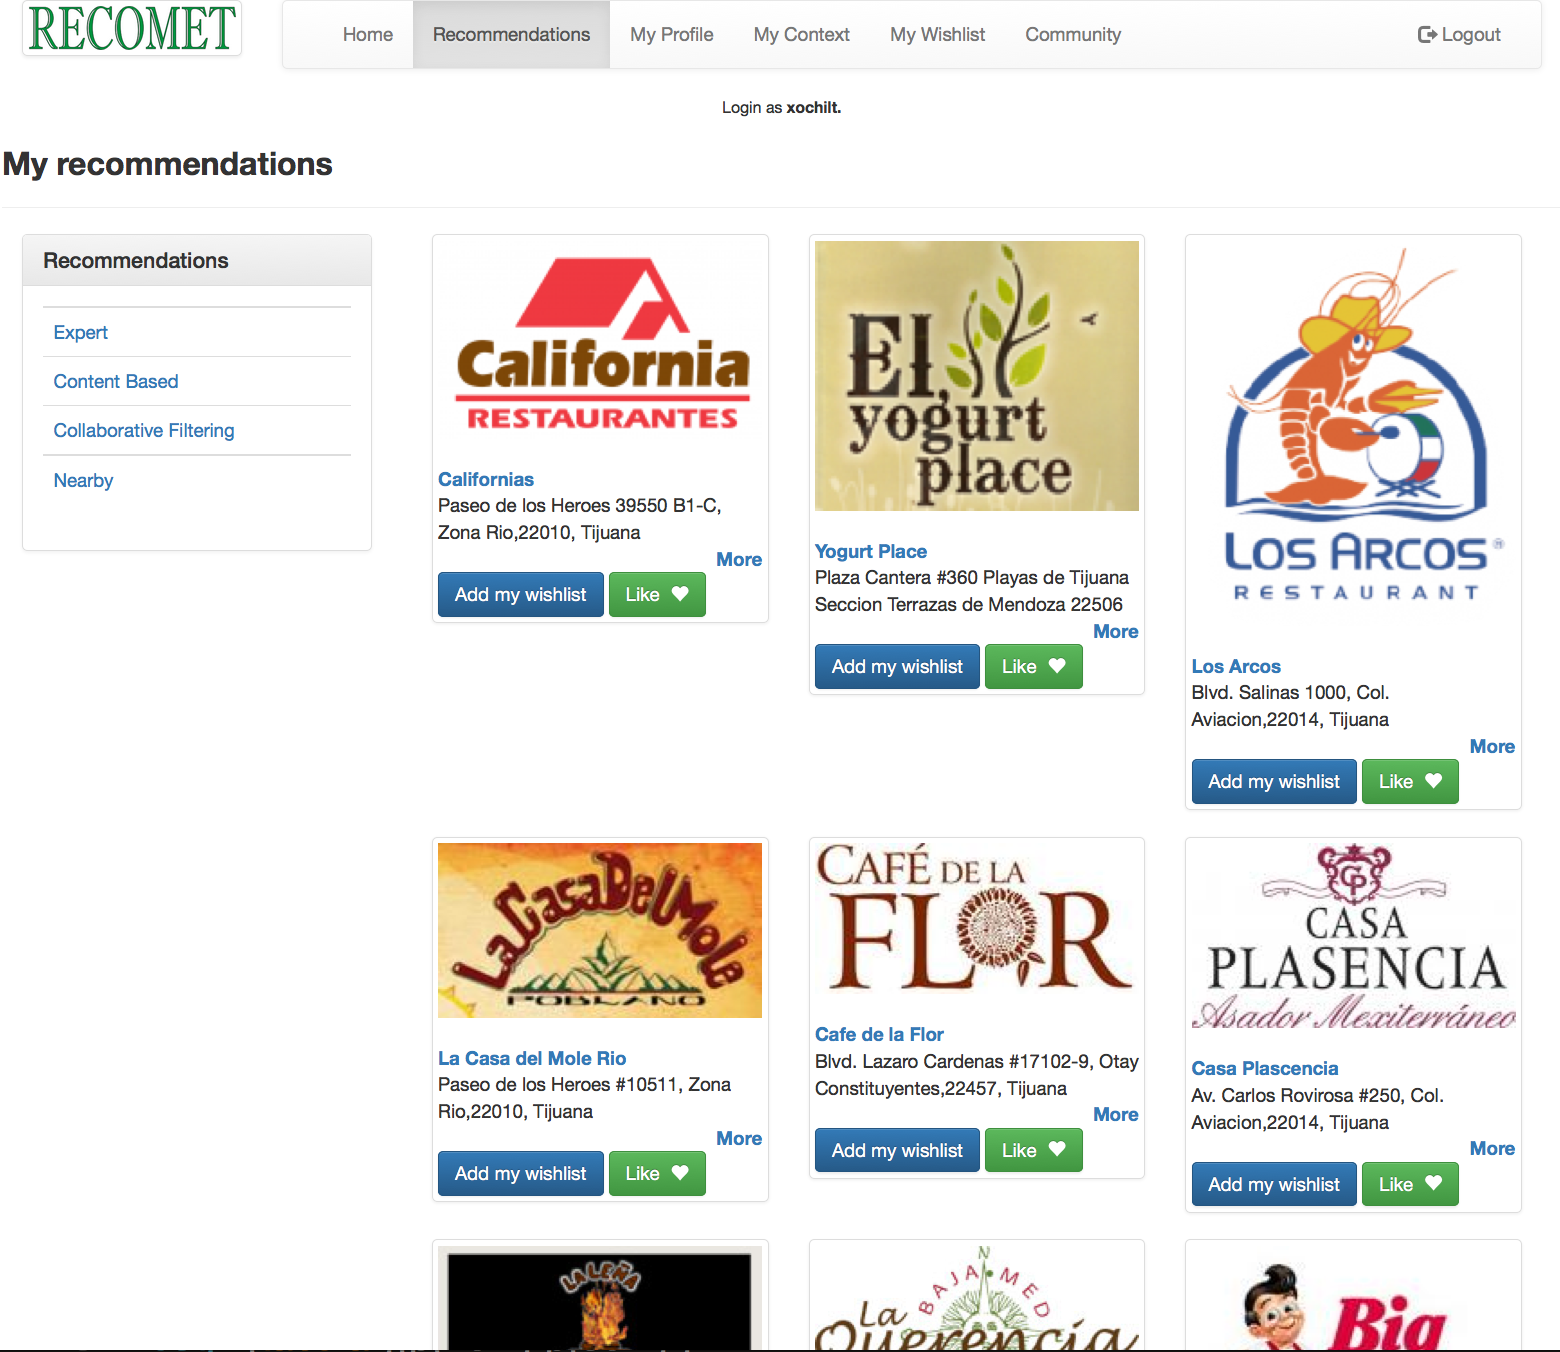
\includegraphics[width=0.70\textwidth]{img/base-content.png}}
\caption{Content-based recommendations interface.}
\label{fig:base-content}   
\end{figure*}
%%%%%%%%%%%%%%%
\textit{Content-based recommendation} finds the similar restaurants to the
favorites of the user. In fact, makes a comparison of all restaurants
and gets the more similars to display in the screen. 
Figure \ref{fig:base-content}  
>>>>>>> origin/master
shows the results of the search, large amount of restaurants are showed
because of the similarity among restaurants, this is the most
efficiently way to get recommendations when the system has not enough
information about user preferences and it the users community is
small. It is not functional whether the user has not at less one vote
<<<<<<< HEAD
with high rating (five stars).\\
\textit{Collaborative filtering recommendation} is depicted in the 
Figure  \ref{fig:cf-recs}
this technique is based in users' opinions, if the system has not
information of users, or whether the users community is small, 
=======
with high rating (5 stars).\\ 
%%%%%%%%%%%%%%%
\textit{Collaborative filtering recommendation} is depicted in the 
figure \ref{fig:cf-recs}
this technique is based in users' opinions, if the system has not
information of users, or whether the user community is small, 
>>>>>>> origin/master
cold-start problem highlights in results. 
\begin{figure*}
\captionsetup{font=footnotesize}
\centering
<<<<<<< HEAD
\fbox{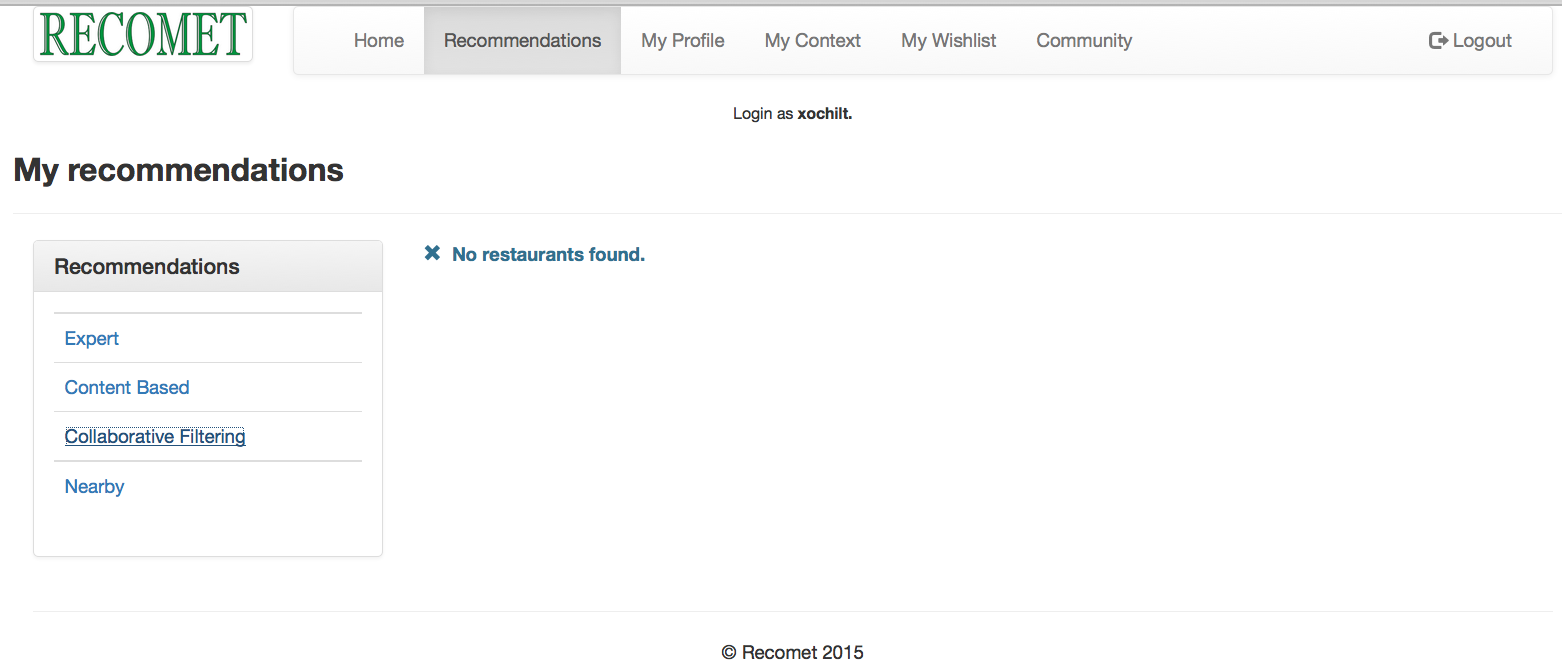
\includegraphics[width=0.60\textwidth]{img/cf-recs.png}}
\caption{Collaborative filtering recommendations interface.}
\label{fig:cf-recs}   
\end{figure*}
\begin{figure*}
\captionsetup{font=footnotesize}
\centering
\fbox{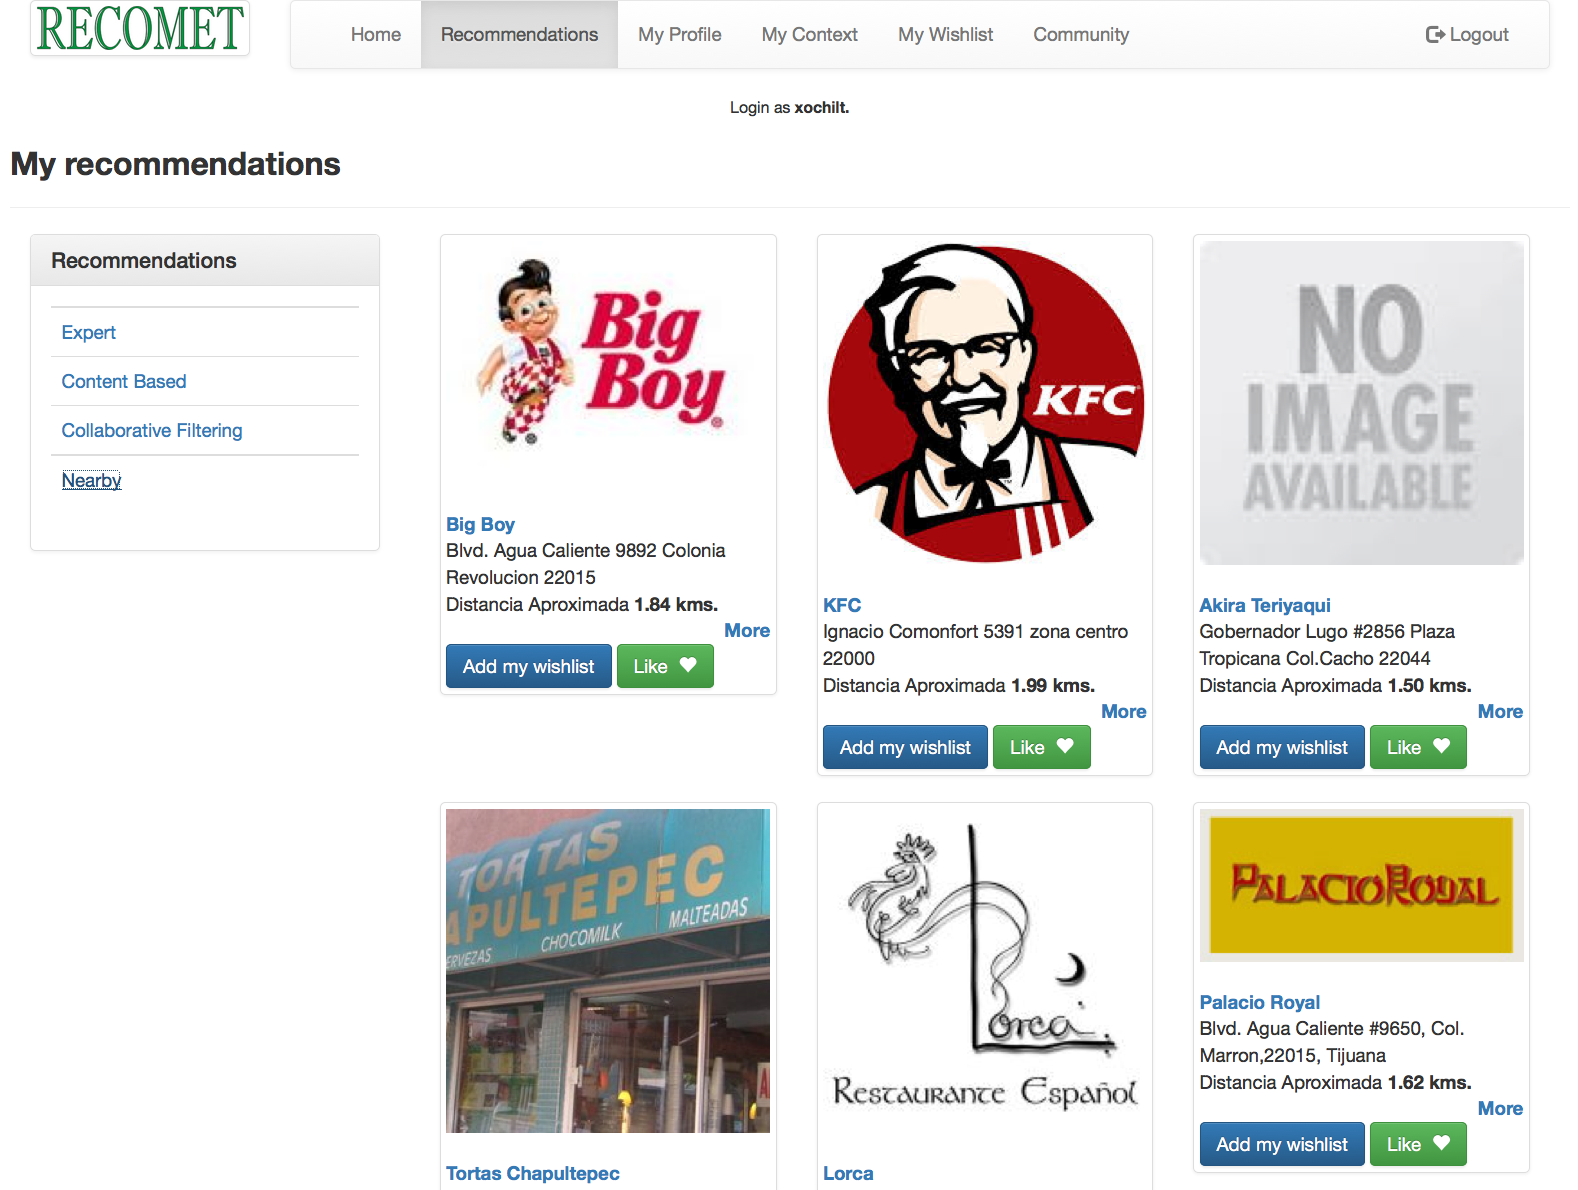
\includegraphics[width=0.60\textwidth]{img/nearby-recs.png}}
\caption{Nearby recommendations interface.}
\label{fig:nearby-recs}   
\end{figure*}
=======
\fbox{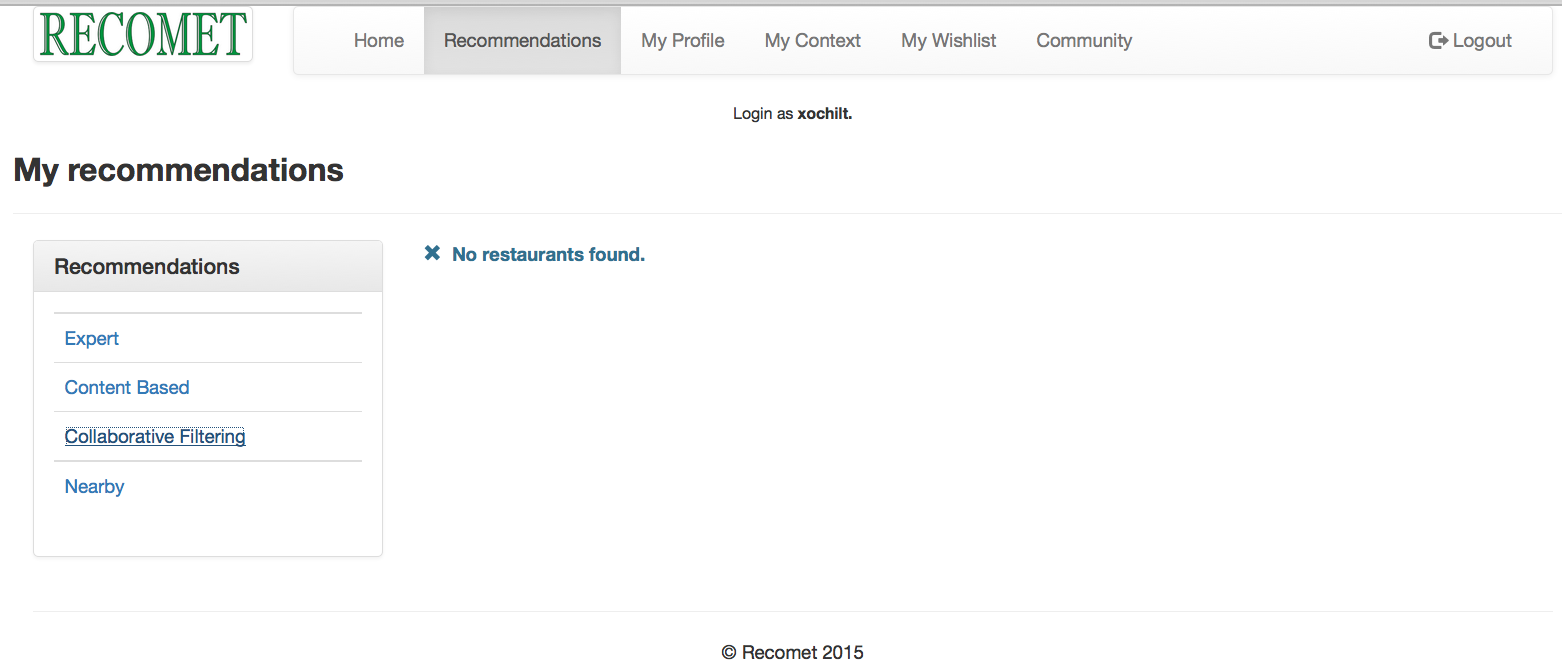
\includegraphics[width=0.70\textwidth]{img/cf-recs.png}}
\caption{Collaborative filtering recommendations interface.}
\label{fig:cf-recs}   
\end{figure*}
>>>>>>> origin/master
As in expert  recommendations if the users participations 
is low or null, the results of recommendations will be empty 
and the alert message appears in the
screen, else, the restaurants suggested will be displayed 
in the screen.\\
<<<<<<< HEAD
\textit{Nearby recommendations} (Figure  \ref{fig:nearby-recs}) 
provides recommendations when the
user previously specifies a geographical position. The distance to
considers restaurants from the current position to two kilometers
around. Then, recommendations are displayed in the screen if the
location is provided in the context, else, an alert message  notifies
the lack of user current location.


\subsubsection{My Profile interface}

\begin{figure*}
\captionsetup{font=footnotesize}
\centering
\fbox{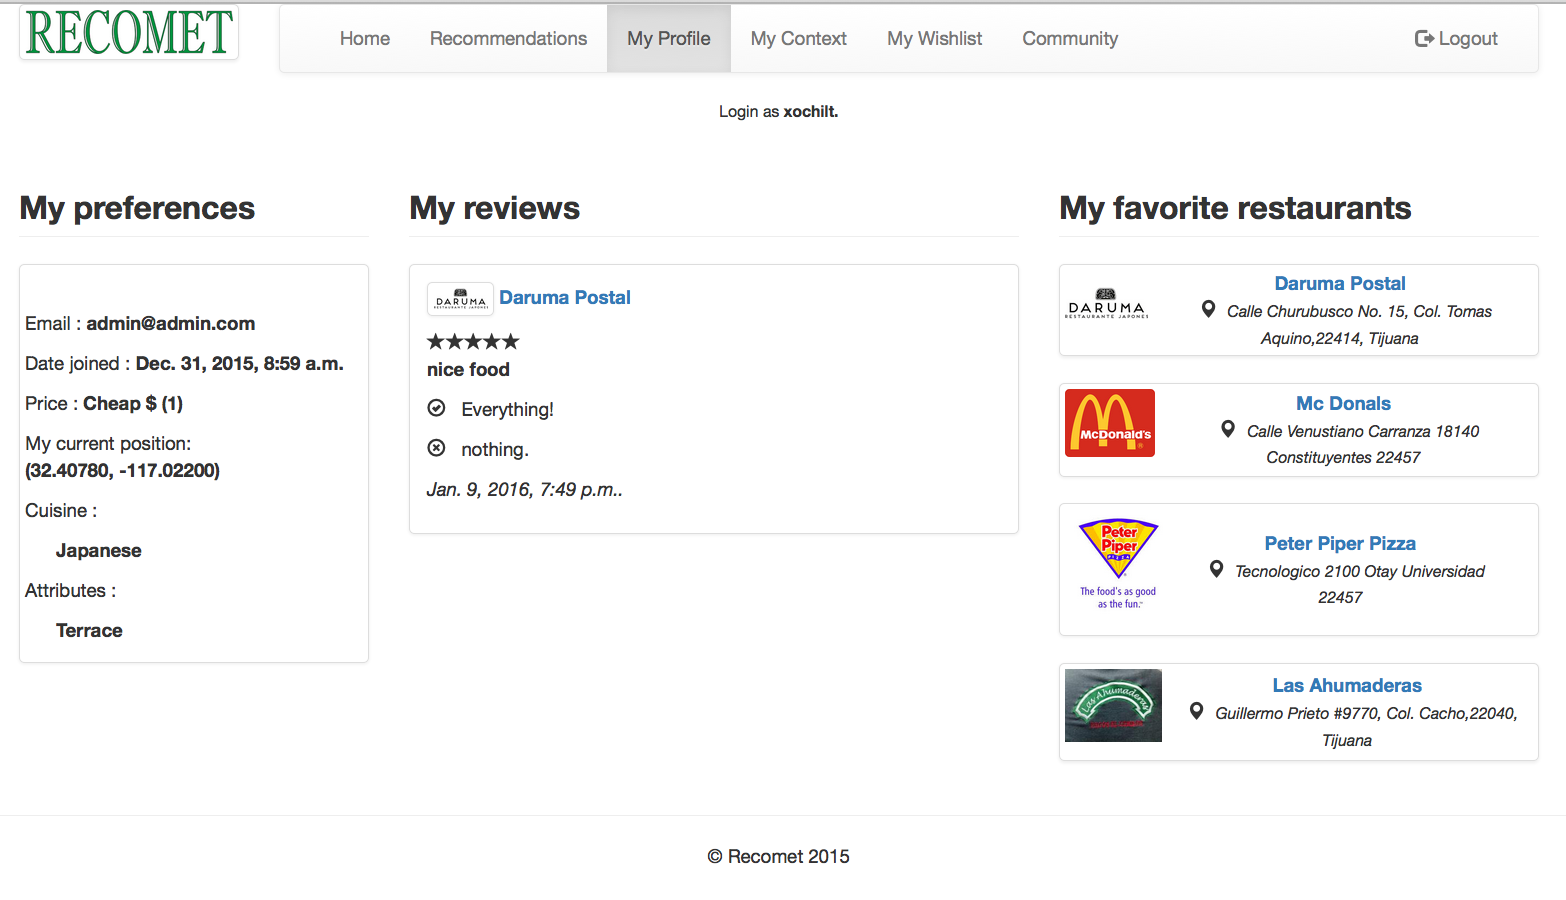
\includegraphics[width=0.60\textwidth]{img/myprofile.png}}
\caption{My Profile interface.}
\label{fig:myprofile}   
\end{figure*}
My Profile interface shows all the information of the user divided in
three sections: my preferences, my reviews and my favorite restaurants
as shown in Figure  \ref{fig:myprofile}. \\The preferences represent the basic
information and tastes of a user, it contains the tastes and preferences
of the user, some factors as price, position, cuisine and attributes
of restaurants could be changing continuosly, it depends how the user
want manage its information.\\ The prototype uses this information every
time that a request of recommendation is done.
The My reviews section shows all the reviews that the user typed, each
review is stored in database and the user cannot delete it. \\The stars
represent the level of satisfaction of the user when he/she visits the
restaurant, each review highlights the good and the bad things that
the user perceives in the visit. \\This information is valuable but,
=======
%%%%%%%%%
\textit{Nearby recommendations} (figure \ref{fig:nearby-recs}) 
provides recommendations when the
user previously specifies a geographical position. The distance to
considers restaurants from the current position to two kilometers
around. Then, recommendations are dis- played in the screen if the
location is provided in the context, else, an alert message  notifies
the lack of user current location.
\begin{figure*}
\captionsetup{font=footnotesize}
\centering
\fbox{\includegraphics[width=0.70\textwidth]{img/nearby-recs.png}}
\caption{Nearby recommendations interface.}
\label{fig:nearby-recs}   
\end{figure*}
%%%%%%%%%%%%%%
\subsubsection{My Profile interface}
%%%%%%%%

My Profile interface shows all the information of the user divided in
three sections: my preferences, my reviews and my favorite restaurants
as shown in figure \ref{fig:myprofile}. The preferences represent the basic
information and tastes of a user, it contains the tastes and preferences
of the user, some factors as price, position, cuisine and attributes
of restaurants could be changing continuosly, it depends how the user
want manage its information. The prototype uses this information every
time that a request of recommendation is done.\\
The My reviews section shows all the reviews that the user typed, each
review is stored in database and the user cannot delete it. The stars
represent the level of satisfaction of the user when he/she visits the
restaurant, each review highlights the good and the bad things that
the user perceives in the visit. This information is valuable but,
>>>>>>> origin/master
unfortunatly this prototype not uses it to infer possible tastes and
preferences and subsequently, recommendations. This process might be a
functionality integrated in the future.\\
My favorite restaurants section, displays restaurants rated with five
stars. It means that are the more important options of the user to
visit in this moment and in the future. These restaurants are related
to the content-based recommendation because are the restaurants with
high rating of this particular user.
<<<<<<< HEAD

\subsubsection{My Context interface}

My Context interface is divided in two sections: contextual 
information and current location as in the Figure  \ref{fig:mycontext}.
Contextual information represents the user preferences, for instance
the price range that wants for a specific ocasion, the attributes are
the characteristics of restaurants, so it selects as many as the user
prefers, the limit is the number of characteristics displayed. 
 \begin{figure*}
\captionsetup{font=footnotesize}
\centering
\fbox{\includegraphics[width=0.60\textwidth]{img/mycontext.png}}
\caption{My Context interface.}
\label{fig:mycontext}   
\end{figure*}
\\The same is for cuisines, a total of 30 type of cuisines were
proposed considering the list of restaurants in the prototype, it can
select as many as the user want.  \\All this information is stored and
displayed in home page also in order to help the user to remember
which is the information that the prototype is using to display
recommendations.\\  Current location section shows the Google map to
display the current location, previously the user ought to confirm
that wants to share the current location. \\  When user click in the
\textit{Save My Location button}, the content in the box of latitude
and longitude will be stored in the database(alert message  confirms
the action) and the status will be modified when user location
changes, then, all the locations stored in database become user's
historical information.

\subsubsection{My Wishlist interface}

\begin{figure*}
\captionsetup{font=footnotesize}
\centering
\fbox{\includegraphics[width=0.60\textwidth]{img/mywishlist.png}}
\caption{My Wishlist interface.}
\label{fig:mywishlist}   
\end{figure*}
My Wishlist interface contains the restaurants that are  considered by
the user as future options to vist  (Figure  \ref{fig:mywishlist})  or
simply to have available information for a particular  ocasion. \\The
wishlist allows the manipulation of restaurants,  it means, user can
add or delete restaurants as many as  he/she wants. \\The wishlist could
be empty or full of  restaurants, this information does not affect any
functionality  of the prototype. \\
Making a comparison with others platforms (for instance 
Amazone), this information allows the user to have the own 
\textit{personalized store}, in terms of products sales, the wishlist 
should be the future products to buy.\\ In a similar way, 
=======
%%%%%%%%%%%%%%%%%%%%%%
\begin{figure*}
\captionsetup{font=footnotesize}
\centering
\fbox{\includegraphics[width=0.70\textwidth]{img/myprofile.png}}
\caption{My Profile interface.}
\label{fig:myprofile}   
\end{figure*}
%%%%%%%%%%%%%%%%%%%%%
%%%%%%%%%%%%%%
\subsubsection{My Context interface}
%%%%%%%%
My Context interface is divided in two sections: contextual 
information and current location as in the figure \ref{fig:mycontext}.
%%%%%%%%%%%%%%%%%%%
\begin{figure*}
\captionsetup{font=footnotesize}
\centering
\fbox{\includegraphics[width=0.70\textwidth]{img/mycontext.png}}
\caption{My Context interface.}
\label{fig:mycontext}   
\end{figure*}
 %%%%%%%%%%%%%%%%%%%
Contextual information represents the user preferences, for instance
the price range that wants for a specific ocasion, the attributes are
the characteristics of restaurants, so it selects as many as the user
prefers, the limit is the number of characteristics displayed. \\ 
The same is for cuisines, a total of 30 type of cuisines were proposed
considering the list of restaurants in the prototype, it can select as
many as the user want.  All this information is stored and displayed
in home page also in order to help the user to remember which is the
information that the prototype is using to display recommendations.\\
%%%%%%%%%%%%%%%%%%%%%%%%%%%
 Current location section shows the Google map to display the 
 current location, previously the user ought to confirm that wants 
 to share the current location. When user click in the 
 \textit{Save My Location button}, the content in the box of latitude 
 and longitude will be stored in the database(alert message 
 confirms the action) and the status will be modified when 
 user location changes, then, all the locations stored in 
 database become user's historical information.
%%%%%%%%%%%%%%%%%%%
\subsubsection{My Wishlist interface}
%%%%%%%%%%%%%%%%%%%
\begin{figure*}
\captionsetup{font=footnotesize}
\centering
\fbox{\includegraphics[width=0.70\textwidth]{img/mywishlist.png}}
\caption{My Wishlist interface.}
\label{fig:mywishlist}   
\end{figure*}
%%%%%%%%%%%%%%%%%%
My Wishlist interface contains the restaurants that are 
considered by the user as future options to vist (figure \ref{fig:mywishlist}) 
or simply to have available information for a particular 
ocasion. The wishlist allows the manipulation of restaurants, 
it means, user can add or delete restaurants as many as 
he/she wants.The wishlist could be empty or full of 
restaurants, this information does not affect any functionality 
of the prototype. \\
Making a comparison with others platforms (for instance 
Amazone), this information allows the user to have the own 
\textit{personalized store}, in terms of products sales, the wishlist 
should be the future products to buy. In a similar way, 
>>>>>>> origin/master
this prototype tries to infer the future tastes of the user 
or what restaurants could visit the user in a close future. \\
To facilitates the addition of restaurants the \textit{Add my wishlist} 
button was added in every restaurant of the home 
<<<<<<< HEAD
page (Figure  \ref{fig:wishlist-home}) and in restaurants 
profiles (Figure  \ref{fig:rest-profile2}).
\begin{figure*}
\captionsetup{font=footnotesize}
\centering
\fbox{\includegraphics[width=0.60\textwidth]{img/wishlist-home.png}}
\caption{Functionality of wishlist button in Home page.}
\label{fig:wishlist-home}   
\end{figure*}

\subsubsection{Community interface}

The Community interface contains the reviews of all the users  
(Figure  \ref{fig:community}) in order to display information that may helps
another users to select any restaurant to visit. \\In the real life, the
persons recommend some or another restaurant in the common  language,
remarking the why the restaurant is good or bad according  their
perception. \\The Community section has the same goal, in fact,  some
reviews could be useful for the other users, this opinion may  express
it through the \textit{Helpful button}.
\begin{figure*}
\captionsetup{font=footnotesize}
\centering
\fbox{\includegraphics[width=0.60\textwidth]{img/community.png}}
\caption{Community interface.}
\label{fig:community}   
\end{figure*}
These are the functionalities in the prototype, in order to validate
the performance, an on-line experiment was realized, the metrics 
of usability applied were Time-taks and Taks-success (mentioned 
in chapter  \ref{introduction}). In the next chapter will be 
explained the tests and the results obtained.
=======
page (see figure \ref{fig:wishlist-home}) and in restaurants 
profiles (see figure \ref{fig:rest-profile2}).
%%%%%%%%%%%%%%%%%%%
\begin{figure*}
\captionsetup{font=footnotesize}
\centering
\fbox{\includegraphics[width=0.70\textwidth]{img/wishlist-home.png}}
\caption{Functionality of wishlist button in Home page.}
\label{fig:wishlist-home}   
\end{figure*}
\subsubsection{Community interface}
%%%%%%%%
The Community interface contains the reviews of all the users (figure
\ref{fig:community}) in order to display information that may helps 
another users to select any restaurant to visit. In the real life, the 
persons recommend some or another restaurant in the common 
language, remarking the why the restaurant is good or bad according 
their perception. The Community section has the same goal, in fact, 
some reviews could be useful for the other users, this opinion may 
express it through the \textit{Helpful button}.
%%%%%%%%%%%%%%%%%%%
\begin{figure*}
\captionsetup{font=footnotesize}
\centering
\fbox{\includegraphics[width=0.70\textwidth]{img/community.png}}
\caption{Community interface.}
\label{fig:community}   
\end{figure*}
%%%%%%%%%%%%%%%%%%%

These are the functionalities in the prototype, in order to validate
the performance, an on-line experiment was realized, the metrics 
of usability applied were Time-taks and Taks-success (mentioned 
in chapter  \ref{introduction}). In the next chapter are 
explained the tests  and the results obtained.
>>>>>>> origin/master








\chapter{System evaluation} \label{evaluation}

Initially most recommenders have been evaluated and ranked on their
prediction power, i.e, their ability to accurately predict the user's
choices. However, it is now widely agreed that accurate predictions
are crucial but insufficient to deploy a good recommendation engine.
In many applications people use a recommendation system for more than
an exact anticipation of their tastes.\\ Users may also be interested
in discovering new items, in rapidly exploring diverse items, in
preserving their privacy, in the fast responses of the system, and
many more properties of the interaction with the recommendation
engine. We must hence identify the set of properties that may
influence the success of a recommender system in the context of a
specific application. Then, we can evaluate how the system performs on
the relevant properties\cite{adomavicius2011context}.\\ In this thesis
it performs the \textbf{on-line experiments}, this is maybe the most
trustworthy experiment because is when the system is  used with
\textbf{real users}, typically \textbf{unaware} of the experiment. In
this type of experiment it is possible to collect only certain types
of data but this experimental design is closest to reality.

\section{Metrics}

For purposes to get real data from user experience, usability is used
as evaluation metric of the context-aware recommender system, the
\textbf{task-success} and \textbf{time-on-task} metrics. \\ 
The \textbf{task-success metric} is perhaps the most widely used
performance metric. It measures how effectively users are able to
complete a given set of tasks.  The \textbf{time-on-task metric} is a
common performance metric that measures how much time is required to
complete a task\cite{albert2013measuring}.\\
The \textbf{task-success} is something that almost anyone can do. 
If the users can't complete their tasks, then something is wrong. 
When the users fail to complete a simple task can be an evidence 
that something needs to be fixed in the recommender system.  \\

The usability test consist of
a list of simple tasks for users that they shall perform in the system
to complete the test. Before to start, a minimal description about the
system for user was explained. The tasks list are the following:

\begin{enumerate} 
\item \textit{Rated a restaurant without context.}
\item \textit{Add context to the user profile.}
\item \textit{Filter restaurants by favorite context.}
\item \textit{Find information of a specific restaurant.}
\item \textit{Find all the reviews of a specific restaurant.} 
\item \textit{Find section of my favorite restaurants.}
\item \textit{Add a review of a restaurant.}
\item \textit{Find the most popular restaurants.}
\item \textit{Add a restaurant to your wishlist.}
\item \textit{Get recommendations based on expert opinion.} 
\item \textit{Get the recommendations content-based.}
\item \textit{Get the collaborative recommendations.}
\item \textit{Get recommendations of the nearby restaurants.}
\end{enumerate} 

\section{Enviromental set up}

Each user did the task list, one by one, with previous instructions.
It gives a brief explanation about the general features of system
before to start. The time average for each user was around 10 minutes
to finished all activities without disruptions.\\  After, the results
was depicted in a chart to observe the user behaviour for each task,
in the figure \ref{fig:tsuccess}  the axis (x, y) represent the task
number and percent of success, respectively. The chart shows that only
3 tasks weren't accomplished successfuly, the task 5, 6 and 7. \\ The
issue with task 5 was that users can not found easily the reviews
section in the interface, the issue in task 7 is derived of task 5
because the user couldn’t find the manner to add a review. The task 6
correspond to the favorite restaurants, but the issue is that it was
confused to chose favorite restaurants in place of wishlist section.
\\ In general, these results mean a possible redisign in the
interfacte to facilitate the performance of these tasks.
\begin{figure*}
%\captionsetup{justification=centering,margin=1cm}
\centering
\captionsetup{font=footnotesize}
\fbox{\includegraphics[scale=0.75]{img/tsuccess.png}} %[width=0.7\textwidth]
\caption{Representation of the percent of success for each task.}
\label{fig:tsuccess}   
\end{figure*}
The time it takes a participant to perform a task says a lot about the
usability of the application. In almost every situation, the faster a
participant can complete a task, the better the experience. In fact,
it would be pretty unusual for a user to complain that a task took
less time than expected \cite{albert2013measuring}.\\ Then, task-on-
time was applied to measure time that an user did the task. A resume
of the time tasks for each user it is in table \ref{tab:datausers},
\textit{null} values mean that the user didn't the task.
\begin{table}
\centering
\small
\captionsetup{font=footnotesize}
\caption{Time on task data for 10 users and 13 tasks. }
\label{tab:datausers}  
\begin{tabular}{lllllllllll}
\hline\noalign{\smallskip}
Task  & Us1  & Us2 & Us3 & Us4 & Us5 & Us6 & Us7 & Us8 & Us9 & Us10 \\
\noalign{\smallskip}\hline\noalign{\smallskip}
1 & 12  & 28 & 24 & 30 & 19 & 33  & 23 & 16 & 5  & 7 \\
2 & 3   & 4  & 17 & 5  & 17 & 134 & 9  & 16 & 12 & 11 \\
3 & 123 & 69 & 159& 53 & 69 & 113 & 44 & 41 & 70 & 98 \\
4 & 20  & 4  & 86 & 40 & 13 & 4   & 17 & 3  & 20 & 3 \\
5 & 50  & 10 & 63 & 50 & 7  & 11  & 10 & 5  & 20 & Null \\
6 & 10  & 30 & 28 & 27 & 5  & 46  & Null  & 7  & Null  & 34 \\
7 & 10  & 20 & 16 & 8  & 15 & Null & 9  & 24 & 16 & 28 \\
8 & 18  & 24 & 10 & 10 & 5  & 3   & 27 & 4  & 5  & 6 \\
9 & 5   & 6  & 31 & 4  & 45 & 9   & 12 & 5  & 3  & 8 \\
10 & 15 & 17 & 15 & 11 & 10 & 19  & 13 & 10 & 20 & 20 \\
11 & 30 & 15 & 20 & 16 & 20 & 22  & 15 & 13 & 18 & 20 \\
12 & 12 & 14 & 19 & 14 & 40 & 10  & 17 & 17 & 15 & 15 \\
13 & 25 & 15 & 15 & 14 & 10 & 10  & 11 & 10 & 10 & 25 \\
\noalign{\smallskip}\hline
\end{tabular}
\end{table}

\section{Results}

To measure the efficiency of the metric it was chose an confidence interval.  In
this way, it is observed the time variability within the same task and  also
helps visualize the difference across tasks to determine whether there is a
statistically significant difference between tasks. The obtained information is
in table \ref{tab:ic}, the median was used to calculate the confidence interval.
\begin{table}
\centering
\small
\captionsetup{font=footnotesize}
\caption{Confidence interval per task with a confidence level of 95\%. }
\label{tab:ic}    
\begin{tabular}{lllll}
\hline\noalign{\smallskip}
Task  & Median & CI 95\% & Upper bound & Lower bound  \\
\noalign{\smallskip}\hline\noalign{\smallskip}
1 &    20         & 5.96  & 25.96 & 14.04  \\
2 &    11.5      & 0.81  & 12.31  & 10.69   \\
3 &    69.5      &  25.57   &  95.07  &  43.93   \\
4 &    15        & 16.34  &  31.34  &  -1.34   \\
5 &    15.5     &  14.84  &  30.34  &  0.66  \\
6 &     27.5    &   11.57  &  39.07  &  15.93    \\
7 &     16       &  5.19  & 21.19  &  10.81   \\
8 &     8         &   5.80  &  13.80  & 2.20 \\
9 &     7         & 9.43  &  16.43  &  -2.43  \\
10 &   15       &   2.44  &  17.44   &  12.56   \\
11 &   19       &  3.00  &  22.00  &  16.00   \\
12 &   14.5    &  5.51  &  20.01  &  8.99   \\
13 &   12.5    &  3.89  &  16.39  &  8.61    \\
\noalign{\smallskip}\hline
\end{tabular}
\end{table}
In the next step the USE \textit{(Usefulnes, Satisfaction, and Ease of
Use)} questionnaire \cite{morris2001experience} was applied in order
to get the user's feedback and comments for to know about the
difficults in the test.  The USE questionnaire consists of 30 rating
scales divided into 4 categories: \textit{Usefulness, Satisfaction,
Ease of Use, and Ease of Learning}. Each is a positive statement to
which the user rates level of agreement on a 7-point Likert scale. The
USE questionnaire(see appendix \ref{appendixb}) allows to get values
for Usefulness, Satisfaction, Ease of Use, and Ease of Learning, the
visualizing the results is in the Fig.\ref{fig:radial} , where the
four axis of the radar chart represent the values of percent which
users rated positively this factors with respect to their interaction
with the context-aware recommender system.  The accurate values are
\textit{Usability 83\%, Satisfaction 84\%, Easy of use  92\%, and Easy
of Learning 81\%.}
\begin{figure*}
\centering
\small
\captionsetup{font=footnotesize}
\includegraphics[width=0.8\textwidth]{img/radial.png}%[scale=0.5]{img/radial.png} 
\caption{\small{The radar chart that depicts the four axis 
evaluated in the questionnaire.}}
\label{fig:radial}   
\end{figure*}



\chapter{Conclusions and future work} \label{conclusions}

We observed the users behaviour to identify the most frecuently difficults and
doubts about tasks. We did a brief interview with users after the test in order
to understand their  feelings or mood, their ideas about the experience, and
overall, their opinion about the context-aware recommender system.  The
conclusions are based in user's comments, then the main errors in the system
interface are summarized in three points:
\begin{enumerate}  
\item  Incomplete information for user, i.e., the system doesn't had enough and clear information to be a friendly interface, and therefore the user couldn't do easily a task.
\item Fails in design, because of unordered elements in the screen, in other words, the elements are not in the correct site into the screen to be easily identified per users.
\item Fails in the language and confusion, because of the english language is not the native language of the users.
\end{enumerate}

The three points mentioned are related to the null values in data table (see
Table \ref{tab:datausers}), some users didn't the task because they were
confused, so they decided to omit the task. The null values weren't took in
account when the median was calculated (see Table \ref{tab:ic}).\\  The USE
questionnaire was useful to identify the weaknesses in the context-aware
recommender system.  The percent is upper of the acceptable (80\%), the results
allow to say that the system has a good performance. \\ For the future work we
proposed to improve the problems found in the user interface, so the proposals
are the following:

\begin{enumerate}  
\item  Redesign the user interface could helps to be more friendly for users. Due to the issues, the redesign involves: 
  \begin{enumerate}  
  \item Analyze the amount of information enough for a easy understanding, i.e., how much information the user needs seeing without overload it.
  \item Modify the tasks descriptions in the most simple way to avoid confusion.
  \item Add more language functionalities for to facilitate the tasks for users.
  \end{enumerate}
\item  To apply the usability test again with the changes in the interface in order to observe the level of improves and to compare the results. 
\item  Apply an statistical test to analize the results.
\item  Add collaborative filtering based on model (matrix factorization technique) within the context-aware recommender system in order to improve the level of user satisfaction in the context. 
\item  Add any contextual factors (such as companion, time of day, budget, etc.) in order to include more context information that could be relevant in the recommendations.
\end{enumerate}


\prefacesection{Publications}
%\begin{singlespace}
\begin{enumerate}
\item \textit{Restaurant Recommendations based on a Domain Model and Fuzzy Rules.  Xochilt Ram\'irez-Garc\'ia, Mario Garc\'ia-Vald\'ez. International Seminar on Computational Intelligence. Tijuana Institute of Technology.  Tijuana Mexico. (2012).}
\item \textit{Post-filtering for a Context-Aware Recommender System. Xochilt Ram\'irez-Garc\'ia, Mario Garc\'ia-Vald\'ez. Recent Advances on Hybrid Approaches for Designing Intelligent Systems . Springer International Publishing Switzerland. (2013).}
\item \textit{Recomendaciones contextuales basadas en el enfoque de post-filtrado. Xochilt Ram\'irez-Garc\'ia, Mario Garc\'ia-Vald\'ez. Modelado computacional de Habilidades Linguisticas y Visuales. Vol.74. Research in Computer Sciences, IPN. 2014.}
\item  \textit{Context-aware Recommender System Based in Pre-filtering Approach and Fuzzy Rules. Xochilt Ram\'irez-Garc\'ia, Mario Garc\'ia-Vald\'ez. Recent Advances on Hybrid Approaches for Designing Intelligent Systems . Springer International Publishing Switzerland. (2014).}
\item  \textit{Context-Aware Recommender System Using Collaborative Filtering, Content-Based Algorithm and Fuzzy Rules. Xochilt Ram\'irez-Garc\'ia, Mario Garc\'ia-Vald\'ez, 2016.}
\item \textit{A Hybrid Context-aware Recommender System for Restaurants. Xochilt Ram\'irez-Garc\'ia, Mario Garc\'ia-Vald\'ez, 2016.}
\end{enumerate}
%\end{singlespace}
\appendix
\chapter{Technical support of installation}\label{appendixa}
%\begin{singlespace}
\textbf{\large{Dependencies of the application}}
\begin{itemize}
\item Django framework 1.7.\\ Url: 
\url{https://www.djangoproject.com/download/}
\item Django-registration library. \\
Url: \url{https://pypi.python.org/pypi/django-registration}
\item Django-countries library. \\
Url: \url{https://pypi.python.org/pypi/django-countries}
\item Django-geoposition library. \\
Url: \url{https://pypi.python.org/pypi/django-geoposition}
\item Python-dateutil library. \\
Url: \url{https://pypi.python.org/pypi/python-dateutil/2.4.1}
\item Pyproj library. \\
Url: \url{https://pypi.python.org/pypi/pyproj?}
\item Numpy library. \\
Url: \url{https://pypi.python.org/pypi/numpy}
\item PostgreSQL database. 
\\Url: \url{http://www.postgresql.org/}
\item Psycopg2 connection to database. \\
Url: \url{http://initd.org/psycopg/docs/install.html}
\item System prototype programmed in Python language 
Url:\url{https://github.com/xochilt/recomet}.
\end{itemize}
%\end{singlespace}
\textbf{\large{Tijuana Restaurants dataset}}

Table \ref{tab:dataset} shows a sample of dataset  where the domain
of contextual factors  is depicted as numeric values, from column 5 to
12  are the contextual factors used in the system and each column
contains the domain values.  The column names are: \textit{payment
type}, \textit{alcohol type}, \textit{smoking area},
\textit{atmosphere type}, \textit{dress code}, \textit{installations
type},\textit{parking type}, and \textit{cuisine type}.
The complete dataset is available to download in the url: 
\url{http://www.xramirezg.wixsite.com/ittresearch}.\\ 
\begin{table}
\small
\captionsetup{font=footnotesize}
\caption{Sample of Tijuana dataset and contextual factors.}
\label{tab:dataset} 
%\centering
\begin{tabular}{lllllllllllll}
\hline\noalign{\smallskip}
Id &  Restaurant & Price & Latitude &  Longitude & 5 & 6 & 7 & 8 & 9 & 10 & 11 & 12   \\
\noalign{\smallskip}\hline\noalign{\smallskip}
1   &   Californias &   3   &   32.52837    &   -117.02001  &   2   &   0   &   1   &   2   &   2   &   1   &   1   &   20  \\
2   &   Yogurt Place    &   2   &   32.53404    &   -117.12053  &   1   &   0   &   1   &   2   &   2   &   1   &   1   &   19  \\
3   &   Los Arcos   &   1   &   32.51582    &   -117.01032  &   2   &   0   &   1   &   2   &   2   &   1   &   1   &   24  \\
4   &   La Casa del Mole &   2   &   32.51995    &   -117.01001  &   2   &   0   &   1   &   2   &   2   &   1   &   1   &   20  \\
5   &   Cafe de la Flor     &   2   &   32.53198    &   -116.94801  &   2   &   0   &   1   &   3   &   2   &   1   &   1   &   16  \\
6   &   Casa Plascencia &   3   &   32.5137 &   -117.00712  &   2   &   0   &   1   &   4   &   2   &   1   &   1   &   22  \\
7   &   La Lena &   3   &   32.51238    &   -117.00417  &   2   &   0   &   1   &   4   &   2   &   1   &   1   &   17  \\
8   &   La Querencia    &   3   &   32.51678    &   -117.00961  &   2   &   0   &   1   &   4   &   2   &   1   &   1   &   22  \\
9   &   Big Boy &   2   &   32.51957    &   -117.01942  &   1   &   0   &   2   &   2   &   2   &   1   &   1   &   26  \\
10  &   Burger King &   1   &   32.53387    &   -116.95086  &   1   &   0   &   2   &   2   &   2   &   1   &   1   &   26  \\
11  &   Cheripan Otay   &   4   &   32.51987    &   -117.01253  &   2   &   0   &   1   &   2   &   2   &   1   &   1   &   4   \\
12  &   Costco  &   1   &   32.50826    &   -116.96436  &   1   &   0   &   2   &   2   &   2   &   1   &   1   &   26  \\
13  &   Daruma Postal   &   2   &   32.52874    &   -116.98579  &   1   &   0   &   2   &   3   &   1   &   1   &   2   &   1   \\
14  &   Dominos Pizza   &   1   &   32.53481    &   -116.97108  &   1   &   0   &   2   &   2   &   2   &   1   &   1   &   27  \\
15  &   El Mazateno &   1   &   32.52836    &   -116.99242  &   2   &   0   &   2   &   3   &   1   &   1   &   2   &   24  \\
16  &   El Porton   &   2   &   32.47732    &   -117.02924  &   2   &   0   &   1   &   4   &   2   &   1   &   1   &   20  \\
17  &   El Rodeo    &   1   &   32.54961    &   -116.90429  &   2   &   0   &   1   &   2   &   2   &   1   &   1   &   17  \\
18  &   Giuseppis Rio   &   4   &   32.53135    &   -116.94833  &   2   &   0   &   1   &   4   &   2   &   1   &   1   &   3   \\
19  &   KFC     &   1   &   32.52821    &   -117.02397  &   1   &   0   &   2   &   2   &   2   &   1   &   1   &   26  \\
20  &   La Torta Plaza  &   1   &   32.53434    &   -117.01821  &   1   &   0   &   2   &   3   &   2   &   1   &   1   &   26  \\
21  &   Landini Ristorante  &   3  &   32.51483   &   -117.01069  &   2   &   0   &   1   &   4   &   3   &   1   &   1   &   3   \\
22  &   Carls jr    &   1   &   32.52973    &   -116.9682   &   1   &   1   &   2   &   2   &   2   &   1   &   1   &   26  \\
23  &   Carnitas Uruapan  &   1   &   32.50907  &   -116.98759  &   2   &   1   &   1   &   3   &   2   &   1   &   1   &   20  \\
24  &   Fonda Argentina &   3   &   32.51339    &   -117.00743  &   2   &   1   &   1   &   3   &   2   &   1   &   1   &   4   \\
25  &   La Espadana &   4   &   32.51786    &   -117.00954  &   2   &   1   &   1   &   4   &   3   &   1   &   1   &   20  \\
\noalign{\smallskip}\hline
\end{tabular}
\end{table}


\chapter{Pseudocode}\label{appendixb}

%%----------------------------------------------------------------------------
%% Get cosine similarity.
%%----------------------------------------------------------------------------
\begin{algorithm}
\caption{Get cosine similarity values.}
\begin{algorithmic} 
\REQUIRE The list of itemProfilesUser and  itemProfilesAll in binary format.
\ENSURE The list of cosine similairty value for each item of 
the itemProfilesUser  
with each element of itemProfilesAll. 
\STATE $allProfiles \leftarrow $[ ]
\FOR {$itemu$ to size of $itemProfilesUser$}
\FOR {$itema$ to size of $itemProfilesAll$}
\IF {$itemu$ = $itema$}
\STATE jump next item
\ELSE
\STATE $cosineSimilarityValue \leftarrow $ among $itemu$ and $itema$
\STATE $itemProfiles \leftarrow itemu, itema, cosineSimilarityValue$
\ENDIF
\ENDFOR
\ENDFOR
\RETURN $allProfiles$
\end{algorithmic}
\end{algorithm}
%%----------------------------------------------------------------------------
%% Collaborative Filtering algorithm.
%%----------------------------------------------------------------------------
\begin{algorithm}
\caption{Collaborative filtering algorithm.}
\begin{algorithmic} 
\REQUIRE The userId.
\ENSURE The Top-N list of recommendations for the current user. 
\STATE $ratingMatrix \leftarrow {allRatings}$
\STATE Call $Recommendations \leftarrow getRecommendations()$ module
\RETURN $Recommendations$
\end{algorithmic}
\end{algorithm}
%%----------------------------------------------------------------------------
%% Content-based algorithm.
%%----------------------------------------------------------------------------
\begin{algorithm}
\small
\caption{Content-based algorithm.}
\begin{algorithmic} 
\REQUIRE The user id.
\ENSURE The Top-N list of recommendations.
\STATE $RV \leftarrow$ All items that user rated with 5
\FOR {$item$ to size of $RV$}
\IF {$item$ is not in $RV$}
\STATE $UV \leftarrow itemid$
\ENDIF
\ENDFOR
\STATE $allItems \leftarrow$ [ ]
\STATE $getItemsProfilesUser \leftarrow$ Binary vectors of RV
\STATE $allRatings \leftarrow$ Rating matrix
\FOR {$item$ to size of $allRatings$}
\IF {$itemid$ is not in $allItems$}
\STATE $allItems \leftarrow item$
\ENDIF
\ENDFOR
\STATE $getAllItemsProfiles \leftarrow$ Binary vectors of allItems
\STATE $getCosineSim \leftarrow$ {{getItemsProfilesUser},{getAllItemsProfiles}}
\FOR {$item$ to size of $highCosineSim$}
\IF {$itemsimilarity \geq  0.8$}
\STATE $highCosineSim \leftarrow item$
\ENDIF
\ENDFOR
\STATE Sort $highCosineSim$ list
\RETURN $itemProfiles$
\end{algorithmic}
\end{algorithm}
%%----------------------------------------------------------------------------
%% Get item profiles used by content-based algorithm.
%%----------------------------------------------------------------------------
\begin{algorithm}
\small
\caption{Get item profiles}
\begin{algorithmic} 
\REQUIRE The UV vector, allItems vector and boolean value of userProfile.
\ENSURE The list of ítemProfiles in binary vectors. 
\IF {$userProfile$ \TRUE }
\STATE $getItemsProfilesUser \leftarrow UV$
\FOR {$itemp$ to size of $UV$}
\STATE get binary vector of itemp
\STATE $itemProfiles \leftarrow itemp$
\ENDFOR
\ELSE
\STATE $allItemProfiles \leftarrow allItems$
\FOR {$itemp$ to size of $allItems$}
\STATE get binary vector of itemp
\STATE $itemProfiles \leftarrow itemp$
\ENDFOR
\ENDIF
\RETURN $itemProfiles$
\end{algorithmic}
\end{algorithm}
%%----------------------------------------------------------------------------
%% Calculate cosine similarity among users.
%%----------------------------------------------------------------------------
\begin{algorithm}
\small
\caption{Calculate Cosine similarity}
\begin{algorithmic} 
\REQUIRE The itemProfileUser and itemProfileAll, both vectors in binary format.
\ENSURE The cosine similarity value.
\STATE $sum \leftarrow 0$
\STATE $normaItemUser \leftarrow 0$
\STATE $normaItemAll \leftarrow 0$
\FOR {$position$ to size of $itemProfileUser$}
\STATE $sumProduct \leftarrow sumProduct+(itemProfileUser[position]*itemProfileAll[position])$
\ENDFOR
\FOR {$item$ to size of $itemProfileUser$}
\STATE $normaItemUser \leftarrow normaItemUser + itemProfileUser[item]^2$
\ENDFOR
\FOR {$item$ to size of $itemProfileAll$}
\STATE $normaItemAll \leftarrow normaItemAll+itemProfileAll[item]^2$
\ENDFOR
\STATE $squareRootUser \leftarrow squareroot(normaItemUser)$
\STATE $squareRootAll   \leftarrow squareroot(normaItemAll)$
\STATE $cosineSimilarity \leftarrow sumProduct/(squareRootUser*squareRootAll)$
\RETURN $cosineSimilarity$
\end{algorithmic}
\end{algorithm}
%%----------------------------------------------------------------------------
%% Create a binary vector of item profile.
%%----------------------------------------------------------------------------
\begin{algorithm}
\caption{Create a binary vector of item profile}
\begin{algorithmic} 
\REQUIRE The ítem profile content in r.
\ENSURE The ítemProfile of r in a binary vector.
\STATE $price \leftarrow $ [4]
\STATE $payment \leftarrow $ [2]
\STATE $alcohol \leftarrow $ [2]
\STATE $smokingarea \leftarrow $ [2]
\STATE $dresscode \leftarrow $ [3]
\STATE $parking \leftarrow $ [3]
\STATE $installation \leftarrow $ [4]
\STATE $atmosphere \leftarrow $ [5]
\STATE $cuisine \leftarrow $ [30]
\STATE $price$[$positionPriceId-1$] $\leftarrow 1$
\STATE $payment$[$positionPriceId-1$] $\leftarrow 1$
\STATE $alcohol$[$positionPriceId-1$] $\leftarrow 1$
\STATE $smokingarea$[$positionPriceId-1$] $\leftarrow 1$
\STATE $dresscode$[$positionPriceId-1$] $\leftarrow 1$
\STATE $parking$[$positionPriceId-1$] $\leftarrow 1$
\STATE $installation$[$positionPriceId-1$] $\leftarrow 1$
\STATE $atmosphere$[$positionPriceId-1$] $\leftarrow 1$
\STATE $cuisine$[$positionPriceId-1$] $\leftarrow 1$
\STATE $itemProfile$ $\leftarrow price+payment+alcohol+smookingarea+dresscode+parking+installation+atmosphere+cuisine$
\RETURN $itemProfile$
\end{algorithmic}
\end{algorithm}
%%----------------------------------------------------------------------------
%% Get recommendations through collabotative filtering.
%%----------------------------------------------------------------------------
\begin{algorithm}
\caption{Get recommendations}
\begin{algorithmic} 
\REQUIRE The currentUser and ratingMatrix.
\ENSURE The Top-N list of recommendations for the current user. 
\STATE Dictionaries $totals \leftarrow \{ \}, sumSimilarity \leftarrow \{ \}$ 
\STATE $predictions \leftarrow $[ ]
\FOR {$otherUser$ to size of $ratingMatrix$}
\IF {$otherUser$ = $currentUser$}
\STATE jump next $otherUser$
\ENDIF
\STATE $similarityValue \leftarrow $ get pearsonSimilarity
\IF {$similarityValue \leq 0 $}
\STATE jump next $otherUser$
\ENDIF
\FOR {$item$ to size of $profileOther$}
\IF {$item$ is not in $profileUser$}
\IF {$profileUser[item]=0$}
\STATE Set in $totals \leftarrow item$
\STATE $totals[item]$ Add $ratingMatrix[otherUser][item]*similarityValue$
\STATE Set in $sunSimilarity \leftarrow item$
\STATE $sumSimilarity$ Add $similarityValue$
\ENDIF
\ENDIF
\ENDFOR
\ENDFOR
\FOR {each $(item,total)$ in $totals$}
\STATE $predictions \leftarrow [(total/sumSimilarity[item], item)]$
\ENDFOR
\STATE Ranking of $predictions$
\RETURN $predictions$
\end{algorithmic}
\end{algorithm}
%%----------------------------------------------------------------------------
%% Get Pearsoncorrelation to get similarity among user neighbors.
%%----------------------------------------------------------------------------
\begin{algorithm}
\caption{Get Pearson correlation}
\begin{algorithmic} 
\REQUIRE The currentUser, otherUser and preferences.
\ENSURE The pearsonCorrelation score.
\STATE Dictionaries $itemsRatedMutually \leftarrow \{ \}$ 
\FOR {each $item$ in preferences of $currentUser$}
\IF {$item$ is in preferences of $currentUser$}
\STATE jump next $itemsRatedMutually[item] \leftarrow 1$
\ENDIF
\ENDFOR
\STATE $numberElements \leftarrow $ size of $itemsRatedMutually$
\IF {$itemsRatedMutually = 0 $}
\RETURN $0$
\ENDIF
\FOR {$item$ to size of $itemsRatedManually$ to get all preferences}
\STATE $sumCurrentUser \leftarrow preferences[currentUser][item]$
\STATE $sumOtherUser \leftarrow preferences[otherUser][item]$
\ENDFOR
\FOR {$item$ to size of $itemsRatedManually$ to get squares}
\STATE $squareCurrentUser \leftarrow square(preferences[currentUser][item])^2$
\STATE $squareOtherUser \leftarrow square(preferences[otherUser][item])^2$
\ENDFOR
\FOR {$item$ to size of $itemsRatedManually$ to get sum of products}
\STATE $sumProduct \leftarrow preferences[currentUser][item]*preferences[otherUser][item]$
\ENDFOR
\STATE $pearsonNumerator \leftarrow sumProduct-((sumCurrentUser*sumOtherUser)/numberElements)$
\STATE $pearsonDenominator \leftarrow square(squareCurrentUser-((sumCurrentUser)^2/numberElements)*squareOtherUser-((sumOtherUser)^2/numberElements))$
\STATE $pearsonCorrelation \leftarrow pearsonNumerator/pearsonDenominator$
\RETURN $pearsonCorrelation$ among two users
\end{algorithmic}
\end{algorithm}
%%----------------------------------------------------------------------------
%% Get factorized matriz for collaborative filtering. Optional use.
%%----------------------------------------------------------------------------
\begin{algorithm}
\caption{Matrix factorization}
\begin{algorithmic}
\REQUIRE R is a matrix to be factorized, dimension N * M, P an initial
matrix of dimension N * K, Q an initial matrix of dimension M * K, K
is the number of latent features, steps for the maximum number of
steps to perform the optimization,  alpha is the learning rate and
beta  is the regularization parameter.
\ENSURE The factorized matrix P and Q.
\STATE $alpha \leftarrow 0.0001, beta \leftarrow 0.001$ 
\STATE $QMatrix \leftarrow QMatrix * T $ 
\FOR {$step$ to $rangeSteps$}
\FOR {$i$ to size of $RMatrix$}
\FOR {$j$ to size of $RMatrix[i]$}
\IF {$RMatrix[i][j] > 0$}
\STATE $e_{i,j} \leftarrow RMatrix[i][j]-dotProduct(PMatrix[i to end],QMatrix[init to j])$
\ENDIF
\FOR {$k$ to range of $KFactors$}
\STATE $PMatrix[i][k] \leftarrow PMatrix[i][k]+alpha * (2*e_{i,j}*QMatrix[k][j] - beta *PMatrix[i][k])$
\STATE $QMatrix[k][j] \leftarrow QMatrix[k][j]+alpha * (2*e_{i,j}*PMatrix[i][k] - beta *QMatrix[k][j])$
\ENDFOR
\ENDFOR
\ENDFOR
\STATE $eR \leftarrow dotProduct (PMatrix * QMatrix)$
\FOR {$i$ to range of $RMatrix$}
\FOR {$j$ to size of $RMatrix[i]$}
\IF {$RMatrix[i][j] > 0$}
\STATE $e \leftarrow e + (beta/2) * PMatrix[i][k]^2 + QMatrix[i][j]^2$
\ENDIF
\ENDFOR
\ENDFOR
\IF {$e < 0$}
\STATE $break$
\ENDIF
\ENDFOR
\RETURN $PMatrix, QMatrix * T$ 
\end{algorithmic}
\end{algorithm}


\textbf{Download Python code:} \url{https://github.com/xochilt/recomet}


\chapter{Technical support of installation}\label{appendixc}
\begin{singlespace}
\textbf{\large{Dependencies of the application}}
\begin{itemize}
\item Django framework 1.7. Url: \textit{https://www.djangoproject.com/download/}
\item Django-registration library. Url: \textit{https://pypi.python.org/pypi/django-registration}
\item Django-countries library. Url: \textit{https://pypi.python.org/pypi/django-countries}
\item Django-geoposition library. Url: \textit{https://pypi.python.org/pypi/django-geoposition}
\item Python-dateutil library. Url: \textit{https://pypi.python.org/pypi/python-dateutil/2.4.1}
\item Pyproj library. Url: \textit{https://pypi.python.org/pypi/pyproj?}
\item Numpy library. Url: \textit{https://pypi.python.org/pypi/numpy}
\item PostgreSQL database. Url: \textit{http://www.postgresql.org/}
\item Psycopg2 connection to database. Url: \textit{http://initd.org/psycopg/docs/install.html}
\end{itemize}
\end{singlespace}

\textbf{\large{Tijuana Restaurants dataset}}

Table \ref{tab:dataset} shows a sample of dataset  where the domain
of contextual factors  is depicted as numeric values, from column 5 to
12  are the contextual factors used in the system and each column
contains the domain values.  The column names are: \textit{payment
type}, \textit{alcohol type}, \textit{smoking area},
\textit{atmosphere type}, \textit{dress code}, \textit{installations
type},\textit{parking type}, and \textit{cuisine type}.
The complete dataset is available to download in the url: 
\url{http://www.xochilt.wix.com/ittresearch}.

\begin{table}
\small
\captionsetup{font=footnotesize}
\caption{Sample of Tijuana dataset and contextual factors.}
\label{tab:dataset} 
\centering
\begin{tabular}{lllllllllllll}
\hline\noalign{\smallskip}
Id &  Restaurant & Price & Latitude &  Longitude & 5 & 6 & 7 & 8 & 9 & 10 & 11 & 12   \\
\noalign{\smallskip}\hline\noalign{\smallskip}
1   &   Californias &   3   &   32.52837    &   -117.02001  &   2   &   0   &   1   &   2   &   2   &   1   &   1   &   20  \\
2   &   Yogurt Place    &   2   &   32.53404    &   -117.12053  &   1   &   0   &   1   &   2   &   2   &   1   &   1   &   19  \\
3   &   Los Arcos   &   1   &   32.51582    &   -117.01032  &   2   &   0   &   1   &   2   &   2   &   1   &   1   &   24  \\
4   &   La Casa del Mole &   2   &   32.51995    &   -117.01001  &   2   &   0   &   1   &   2   &   2   &   1   &   1   &   20  \\
5   &   Cafe de la Flor     &   2   &   32.53198    &   -116.94801  &   2   &   0   &   1   &   3   &   2   &   1   &   1   &   16  \\
6   &   Casa Plascencia &   3   &   32.5137 &   -117.00712  &   2   &   0   &   1   &   4   &   2   &   1   &   1   &   22  \\
7   &   La Lena &   3   &   32.51238    &   -117.00417  &   2   &   0   &   1   &   4   &   2   &   1   &   1   &   17  \\
8   &   La Querencia    &   3   &   32.51678    &   -117.00961  &   2   &   0   &   1   &   4   &   2   &   1   &   1   &   22  \\
9   &   Big Boy &   2   &   32.51957    &   -117.01942  &   1   &   0   &   2   &   2   &   2   &   1   &   1   &   26  \\
10  &   Burger King &   1   &   32.53387    &   -116.95086  &   1   &   0   &   2   &   2   &   2   &   1   &   1   &   26  \\
11  &   Cheripan Otay   &   4   &   32.51987    &   -117.01253  &   2   &   0   &   1   &   2   &   2   &   1   &   1   &   4   \\
12  &   Costco  &   1   &   32.50826    &   -116.96436  &   1   &   0   &   2   &   2   &   2   &   1   &   1   &   26  \\
13  &   Daruma Postal   &   2   &   32.52874    &   -116.98579  &   1   &   0   &   2   &   3   &   1   &   1   &   2   &   1   \\
14  &   Dominos Pizza   &   1   &   32.53481    &   -116.97108  &   1   &   0   &   2   &   2   &   2   &   1   &   1   &   27  \\
15  &   El Mazateno &   1   &   32.52836    &   -116.99242  &   2   &   0   &   2   &   3   &   1   &   1   &   2   &   24  \\
16  &   El Porton   &   2   &   32.47732    &   -117.02924  &   2   &   0   &   1   &   4   &   2   &   1   &   1   &   20  \\
17  &   El Rodeo    &   1   &   32.54961    &   -116.90429  &   2   &   0   &   1   &   2   &   2   &   1   &   1   &   17  \\
18  &   Giuseppis Rio   &   4   &   32.53135    &   -116.94833  &   2   &   0   &   1   &   4   &   2   &   1   &   1   &   3   \\
19  &   KFC     &   1   &   32.52821    &   -117.02397  &   1   &   0   &   2   &   2   &   2   &   1   &   1   &   26  \\
20  &   La Torta Plaza  &   1   &   32.53434    &   -117.01821  &   1   &   0   &   2   &   3   &   2   &   1   &   1   &   26  \\
21  &   Landini Ristorante  &   3  &   32.51483   &   -117.01069  &   2   &   0   &   1   &   4   &   3   &   1   &   1   &   3   \\
22  &   Carls jr    &   1   &   32.52973    &   -116.9682   &   1   &   1   &   2   &   2   &   2   &   1   &   1   &   26  \\
23  &   Carnitas Uruapan  &   1   &   32.50907  &   -116.98759  &   2   &   1   &   1   &   3   &   2   &   1   &   1   &   20  \\
24  &   Fonda Argentina &   3   &   32.51339    &   -117.00743  &   2   &   1   &   1   &   3   &   2   &   1   &   1   &   4   \\
25  &   La Espadana &   4   &   32.51786    &   -117.00954  &   2   &   1   &   1   &   4   &   3   &   1   &   1   &   20  \\
\noalign{\smallskip}\hline
\end{tabular}
\end{table}


%\chapter{System interfaces}\label{appendixd}

\begin{figure}[ht!]
   \captionsetup{font=footnotesize}
   \centering
   %%----primera subfigura----
   \subfloat[]{
    \label{fig:a}
    \fbox{\includegraphics[width=0.7\textwidth]{img/recomet-home.png}}}
   \hspace{0.01\linewidth}
   %%----segunda subfigura----
   % \subfloat[]{
   %      \label{fig:mf:b} 
   %      \fbox{\includegraphics[width=6.5cm]{img/recomet-recom.png}}}
   \caption{Home interface of the system.
   }
   \label{fig:home} 
\end{figure}

\begin{figure}[ht!]
   \captionsetup{font=footnotesize}
   \centering
   %%----primera subfigura----
   \subfloat[]{
        \label{fig:mf:a}
        \fbox{\includegraphics[width=0.7\textwidth]{img/recomet-myprofile.png}}}
   \hspace{0.1\linewidth}
   %%----segunda subfigura----
   \subfloat[]{
        \label{fig:mf:b} 
       \fbox{ \includegraphics[width=0.7\textwidth]{img/recomet-wishlist.png}}}\\[20pt]
   %%----tercera subfigura----
   % \subfloat[]{
   %      \label{fig:mf:c} 
   %      \includegraphics[width=0.6\textwidth]{img/recomet-wishlist.png}}
    %\hspace{0.1\linewidth}
   \caption{a)\textit{My profile} and b)\textit{My wishlist} interfaces of the system.
   }
   \label{fig:wishlist} 
\end{figure}


%% Cap'itulos incluidos despues del comando \appendix aparecen como ap'endices
%% de la tesis.
%% bibliography
\bibliographystyle{ieeetr}
\bibliography{biblio}
\end{document}
